\documentclass[unicode,11pt,a4paper,oneside,numbers=endperiod,openany]{scrartcl}
\usepackage[fleqn]{amsmath}

\usepackage{xcolor}
\renewcommand{\thesubsection}{\arabic{subsection}}

\usepackage{ifthen}
\usepackage[utf8]{inputenc}
\usepackage{graphics}
\usepackage{graphicx}
\usepackage{hyperref}
\usepackage{amsmath}

\pagestyle{plain}
\voffset -5mm
\oddsidemargin  0mm
\evensidemargin -11mm
\marginparwidth 2cm
\marginparsep 0pt
\topmargin 0mm
\headheight 0pt
\headsep 0pt
\topskip 0pt        
\textheight 255mm
\textwidth 165mm

\newcommand{\duedate} {}
\newcommand{\setduedate}[1]{%
\renewcommand\duedate {Due date:~ #1}}
\newcommand\isassignment {false}
\newcommand{\setassignment}{\renewcommand\isassignment {true}}
\newcommand{\ifassignment}[1]{\ifthenelse{\boolean{\isassignment}}{#1}{}}
\newcommand{\ifnotassignment}[1]{\ifthenelse{\boolean{\isassignment}}{}{#1}}

\newcommand{\assignmentpolicy}{
\begin{table}[h]
\begin{center}
\scalebox{0.8} {%
\begin{tabular}{|p{0.02cm}p{16cm}|}
\hline
&\\
\multicolumn{2}{|c|}{\Large\textbf{Numerical Computing 2022 ---  Submission Instructions}}\\
\multicolumn{2}{|c|}{\large\textbf{(Please, notice that following instructions are mandatory: }}\\
\multicolumn{2}{|c|}{\large\textbf{submissions that don't comply with, won't be considered)}}\\
&\\
\textbullet & Assignments must be submitted to \href{https://www.icorsi.ch/course/view.php?id=14666}{iCorsi} (i.e. in electronic format).\\
\textbullet & Provide both executable package and sources (e.g. C/C++ files, Julia). 
If you are using libraries, please add them in the file. Sources must be organized in directories called:\\
\multicolumn{2}{|c|}{\textit{Project\_number\_lastname\_firstname}}\\
& and  the  file must be called:\\
\multicolumn{2}{|c|}{\textit{project\_number\_lastname\_firstname.zip}}\\
\multicolumn{2}{|c|}{\textit{project\_number\_lastname\_firstname.pdf}}\\
\textbullet &  The TAs will grade your project by reviewing your project write-up, and looking at the implementation you attempted, and benchmarking your code's performance.\\

\textbullet & You are allowed to discuss all questions with anyone you like; however: (i) your submission must list anyone you discussed problems with and (ii) you must write up your submission independently.\\
\hline
\end{tabular}
}
\end{center}
\end{table}
}
\newcommand{\punkte}[1]{\hspace{1ex}\emph{\mdseries\hfill(#1~\ifcase#1{Points}\or{Points}\else{Points}\fi)}}


\newcommand\serieheader[6]{
\thispagestyle{empty}%
\begin{flushleft}

\includegraphics[width=0.45\textwidth]{CI_logo}
\end{flushleft}
  \noindent%
  {\large\ignorespaces{\textbf{#1}}\hspace{\fill}\ignorespaces{ \textbf{#2}}}\\ \\%
  {\large\ignorespaces #3 \hspace{\fill}\ignorespaces #4}\\
  \noindent%
  \bigskip
  \hrule\par\bigskip\noindent%
  \bigskip {\ignorespaces {\Large{\textbf{#5}}}
  \hspace{\fill}\ignorespaces \large \ifthenelse{\boolean{\isassignment}}{\duedate}{#6}}
  \hrule\par\bigskip\noindent%  \linebreak
 }

\makeatletter
\def\enumerateMod{\ifnum \@enumdepth >3 \@toodeep\else
      \advance\@enumdepth \@ne
      \edef\@enumctr{enum\romannumeral\the\@enumdepth}\list
      {\csname label\@enumctr\endcsname}{\usecounter
        {\@enumctr}%%%? the following differs from "enumerate"
	\topsep0pt%
	\partopsep0pt%
	\itemsep0pt%
	\def\makelabel##1{\hss\llap{##1}}}\fi}
\let\endenumerateMod =\endlist
\makeatother




\usepackage{textcomp}

% Math
\usepackage[fleqn]{amsmath}
\usepackage{amssymb}
\usepackage{dsfont}
\usepackage{float}


% Allows to use caption*
\usepackage{caption}
% Scalabale subfigures
\usepackage{subcaption} 
% Code syntax highlighting
\usepackage{minted}
% Hyperlinks
\usepackage{hyperref}


\newcommand{\bmat}[1]{
   \ensuremath{
   \begin{bmatrix}
       #1
   \end{bmatrix}
}}



\hyphenation{PageRank}
\hyphenation{PageRanks}


\begin{document}


\setassignment
\setduedate{Wednesday, 23 November 2022, 23:59 AM}

\serieheader{Numerical Computing}{2022}{Student: Albert Cerfeda}{}{Solution for Project 4}{}
\newline

\assignmentpolicy
\tableofcontents
\newpage

\section{Spectral clustering of non-convex sets [50 points]}
\subsection*{1.1. Plotting non-convex sets}
Let us plot the 'Two spirals' non-convex\footnote{Convex sets: In Euclidean space, an object is convex if, given any two points inside the object, the line between them is also within the object. [Source: \href{https://web.stanford.edu/class/ee364a/lectures/sets.pdf}{stanford.edu}]} graph:\\
% TODO: Add ref to table
\begin{figure}[h!]
    \centering
    \includegraphics[height=0.4\linewidth]{fig/1/1.'pts_spiral'.png}
    \caption{$\texttt {pts\_spiral}$ graph.}
    \label{fig:pts_spiral}
\end{figure}\\
By briefly looking at the graph we can easily identify the two main clusters: the two interleaved spirals that meet in the center of the cartesian plane at coordinates $(0,0)$.\\
For us it is intuitive to cluster points that have spacial continuity to each other like in this case, but each clustering algorithm might consider different factors for determining what makes two points 'similar' and therefore belonging to the same cluster.\\\\
The $k$-means algorithm on the eigenvectors of the graph's Laplacian matrix (\textit{Spectral method}) makes the cluster centroids adjust based on the Eigenvector coordinates. As a result the Spectral method values the relative distance between the points, and the two resulting clusters are the ones we are able to identify intuitively. Calculating eigenvectors and eigenvalues of large graphs can get computationally expensive. Fortunately there are efficient methods for calculating the first $K$ eigenvectors of sparse matrices. \\\\
On the other hand, running the standard $k$-means algorithm yields two clusters where we can roughly guess the position of each cluster's centroid is, as they adjust based on the "raw" input graph points. We notice how standard $k$-means method struggles correctly clustering non-convex\footnotemark[1] sets. \\

\clearpage
\subsection*{1.2. Computing the $\epsilon$ factor for $K=2$ and $K=4$ clusters}
As we have a set of points in space, we need to define a function to define and compute the similarity of any two points in the set, fundamental for our clustering algorithms.\\
We define the \textit{Gaussian kernel similarity function} as follows:
\begin{figure}[h!]
$$ s\left(x_i, x_j\right)=e^{\frac{-\left\|x_i-x_j\right\|^2}{2 \sigma^2}}$$
\caption{The \textit{Gaussian Kernel} similarity function}
\end{figure}
Opposed to the \textit{Euclidean distance} function that measures the \textit{distance} between two points, the Gaussian kernel similarity function ranges between $0$ and $1$ as it expresses absolute \textit{similarity} and decreases with distance.\\ 

By using the \textit{Gaussian Similarity function} we define the weighted adjacency matrix $S$ that expresses the gaussian similarity between the points in our set.\\
The choice of the sigma $\sigma$ parameter is important. It controls the size of the neighborhood therefore it allows us to have a more densely connected graph or the opposite. W chose it to be $\mathbf{2*\log n}$.\\

Afterwards we compute the minimal spanning tree\footnote{Minimal Spanning Tree (MST): A subgraph that includes every vertex of the graph with the minimum number of edges, the minimal amount of summed edge weights and that does not contain loops. } of matrix $S$, useful to simplify the graph by removing redundant edges that could hinder our cluster computation.\\

We can finally choose our $\epsilon$ factor for the $\epsilon$-similarity graph. \\
In order for the resulting graph to be safely connected we choose it to be the longest edge in the previously-computed Minimal Spanning Tree.
\begin{figure}[h!]
\begin{minted}[frame=lines,framesep=2mm,]{julia}
# ...
mintree = minspantree(S)
e = maximum(mintree)
# ...
\end{minted}
\caption{Julia code for computing the Minimal Spanning Tree and the $\epsilon$ factor.}
\end{figure}\\
Choosing $\epsilon$ to be the maximum value in the minimum spanning tree of the Gaussian Similarity matrix yields the following results:\\
\textbf{Note}: there is a random component as the datasets are generated at runtime, so results may vary.
\begin{table}[h!]
    \centering
    \begin{tabular}{l|ll}
        Mesh & $\epsilon$ factor \\
        \hline
        \verb|pts_spiral| & $0.8729153954604377$ \\ 
        \verb|pts_clusterin| & $0.8834278441571511$ \\
        \verb|pts_corn| & $0.8623495359026014$ \\
        \verb|pts_halfk| & $0.8735819886907046$ \\
        \verb|pts_moon| & $0.8637545218347059$ \\
        \verb|pts_outlier| & $0.7459541372062404$ \\
    \end{tabular}
    \caption{$\epsilon$ factors for the various graphs}
\end{table}


\clearpage
\subsection*{1.3. Generating the $\epsilon$ similarity graphs}
We first need to compute the $\epsilon$-neighborhood graph $G\in \mathbb{R}^{n\times n}$ defined as follows:\\
\begin{equation}
g_{ij} = \begin{cases}
    1, \quad \text{if }
    
    \underbrace{\sqrt{\sum_{i=1}^{n}(x_i - y_i)^2} }_\text{Euclidean Distance} < \epsilon
    \\\\
    0 \quad \text{otherwise}
\end{cases}
\end{equation}
We can see how our $\epsilon$ factor is used for connecting only vertices whose distance is less than our $\epsilon$ factor.
\begin{figure}[h!]
\begin{minted}[
frame=lines,
framesep=2mm,
]{julia}
function epsilongraph(epsilon, pts)
    n = size(pts, 1);
    G = zeros(n, n);
    for i = 1:n
        for j = 1:n
            if norm(pts[i,:]-pts[j,:]) < epsilon
                G[i,j] = 1
            end
        end
    end
    return sparse(G)
end
# ...
G_e = epsilongraph(e, pts)
\end{minted}
\caption{Julia code defining the function for computing the $\epsilon$-neighborhood graph}
\end{figure}
\subsection*{1.4. Computing and visualizing the adjacency matrix for the $\epsilon$ similarity graph}

Once we multiply the resulting $\epsilon$-neighborhood graph $G$ with our Gaussian Similarity matrix $S$ we obtain the weighted adjacency matrix for the $\epsilon$-neighborhood graph. Like this we make sure to only include the edges that fall under the upperbound imposed by the threshold value $\epsilon$.
\begin{minted}[
frame=lines,
framesep=2mm,
]{julia}
# Create the adjacency matrix for the epsilon case
W_e = S .* G_e;
draw_graph(W_e, pts)
\end{minted}
Let us plot the adjacency matrices for some $\epsilon$-neighborhood graphs:
\begin{figure}[h!]
    \begin{minipage}{0.5\textwidth}
        \centering
        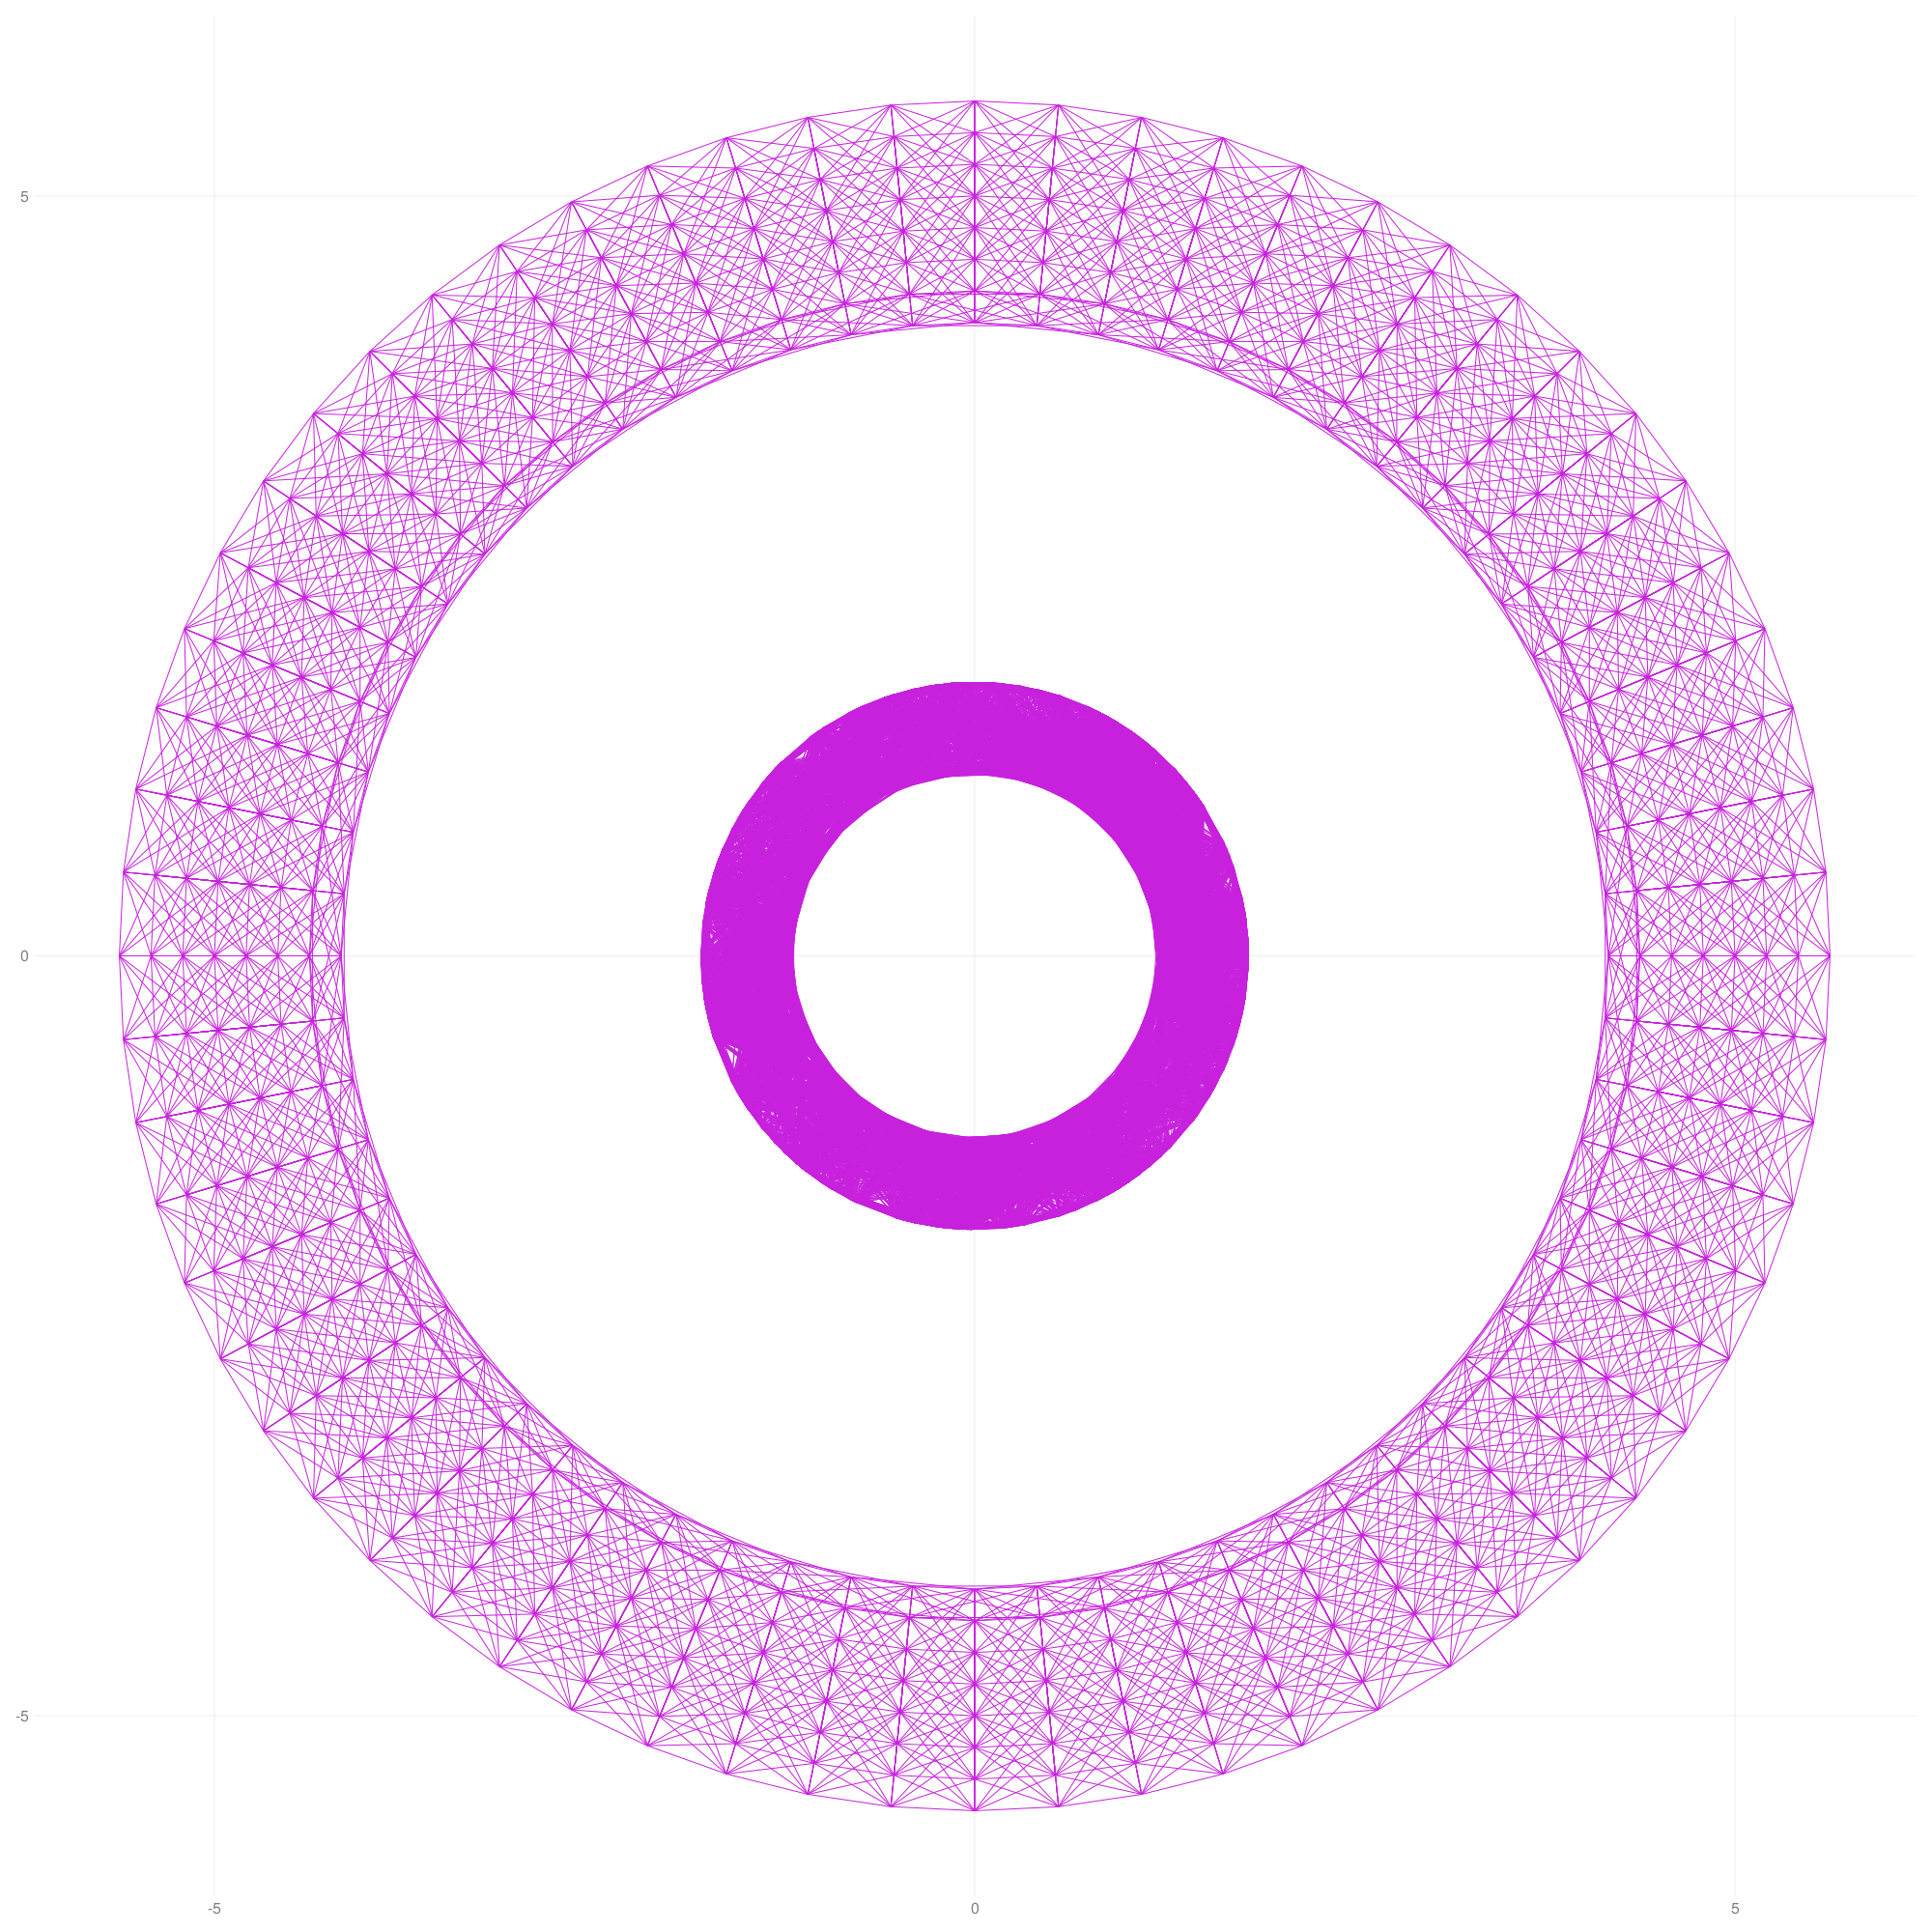
\includegraphics[width=0.5\linewidth]{fig/1/4.'pts_clusterin'-epsilon-adjacency.png}
        \caption{$\texttt {pts\_clusterin }\epsilon$ adjacency graph.}
    \end{minipage}
        \begin{minipage}{0.5\textwidth}
        \centering
        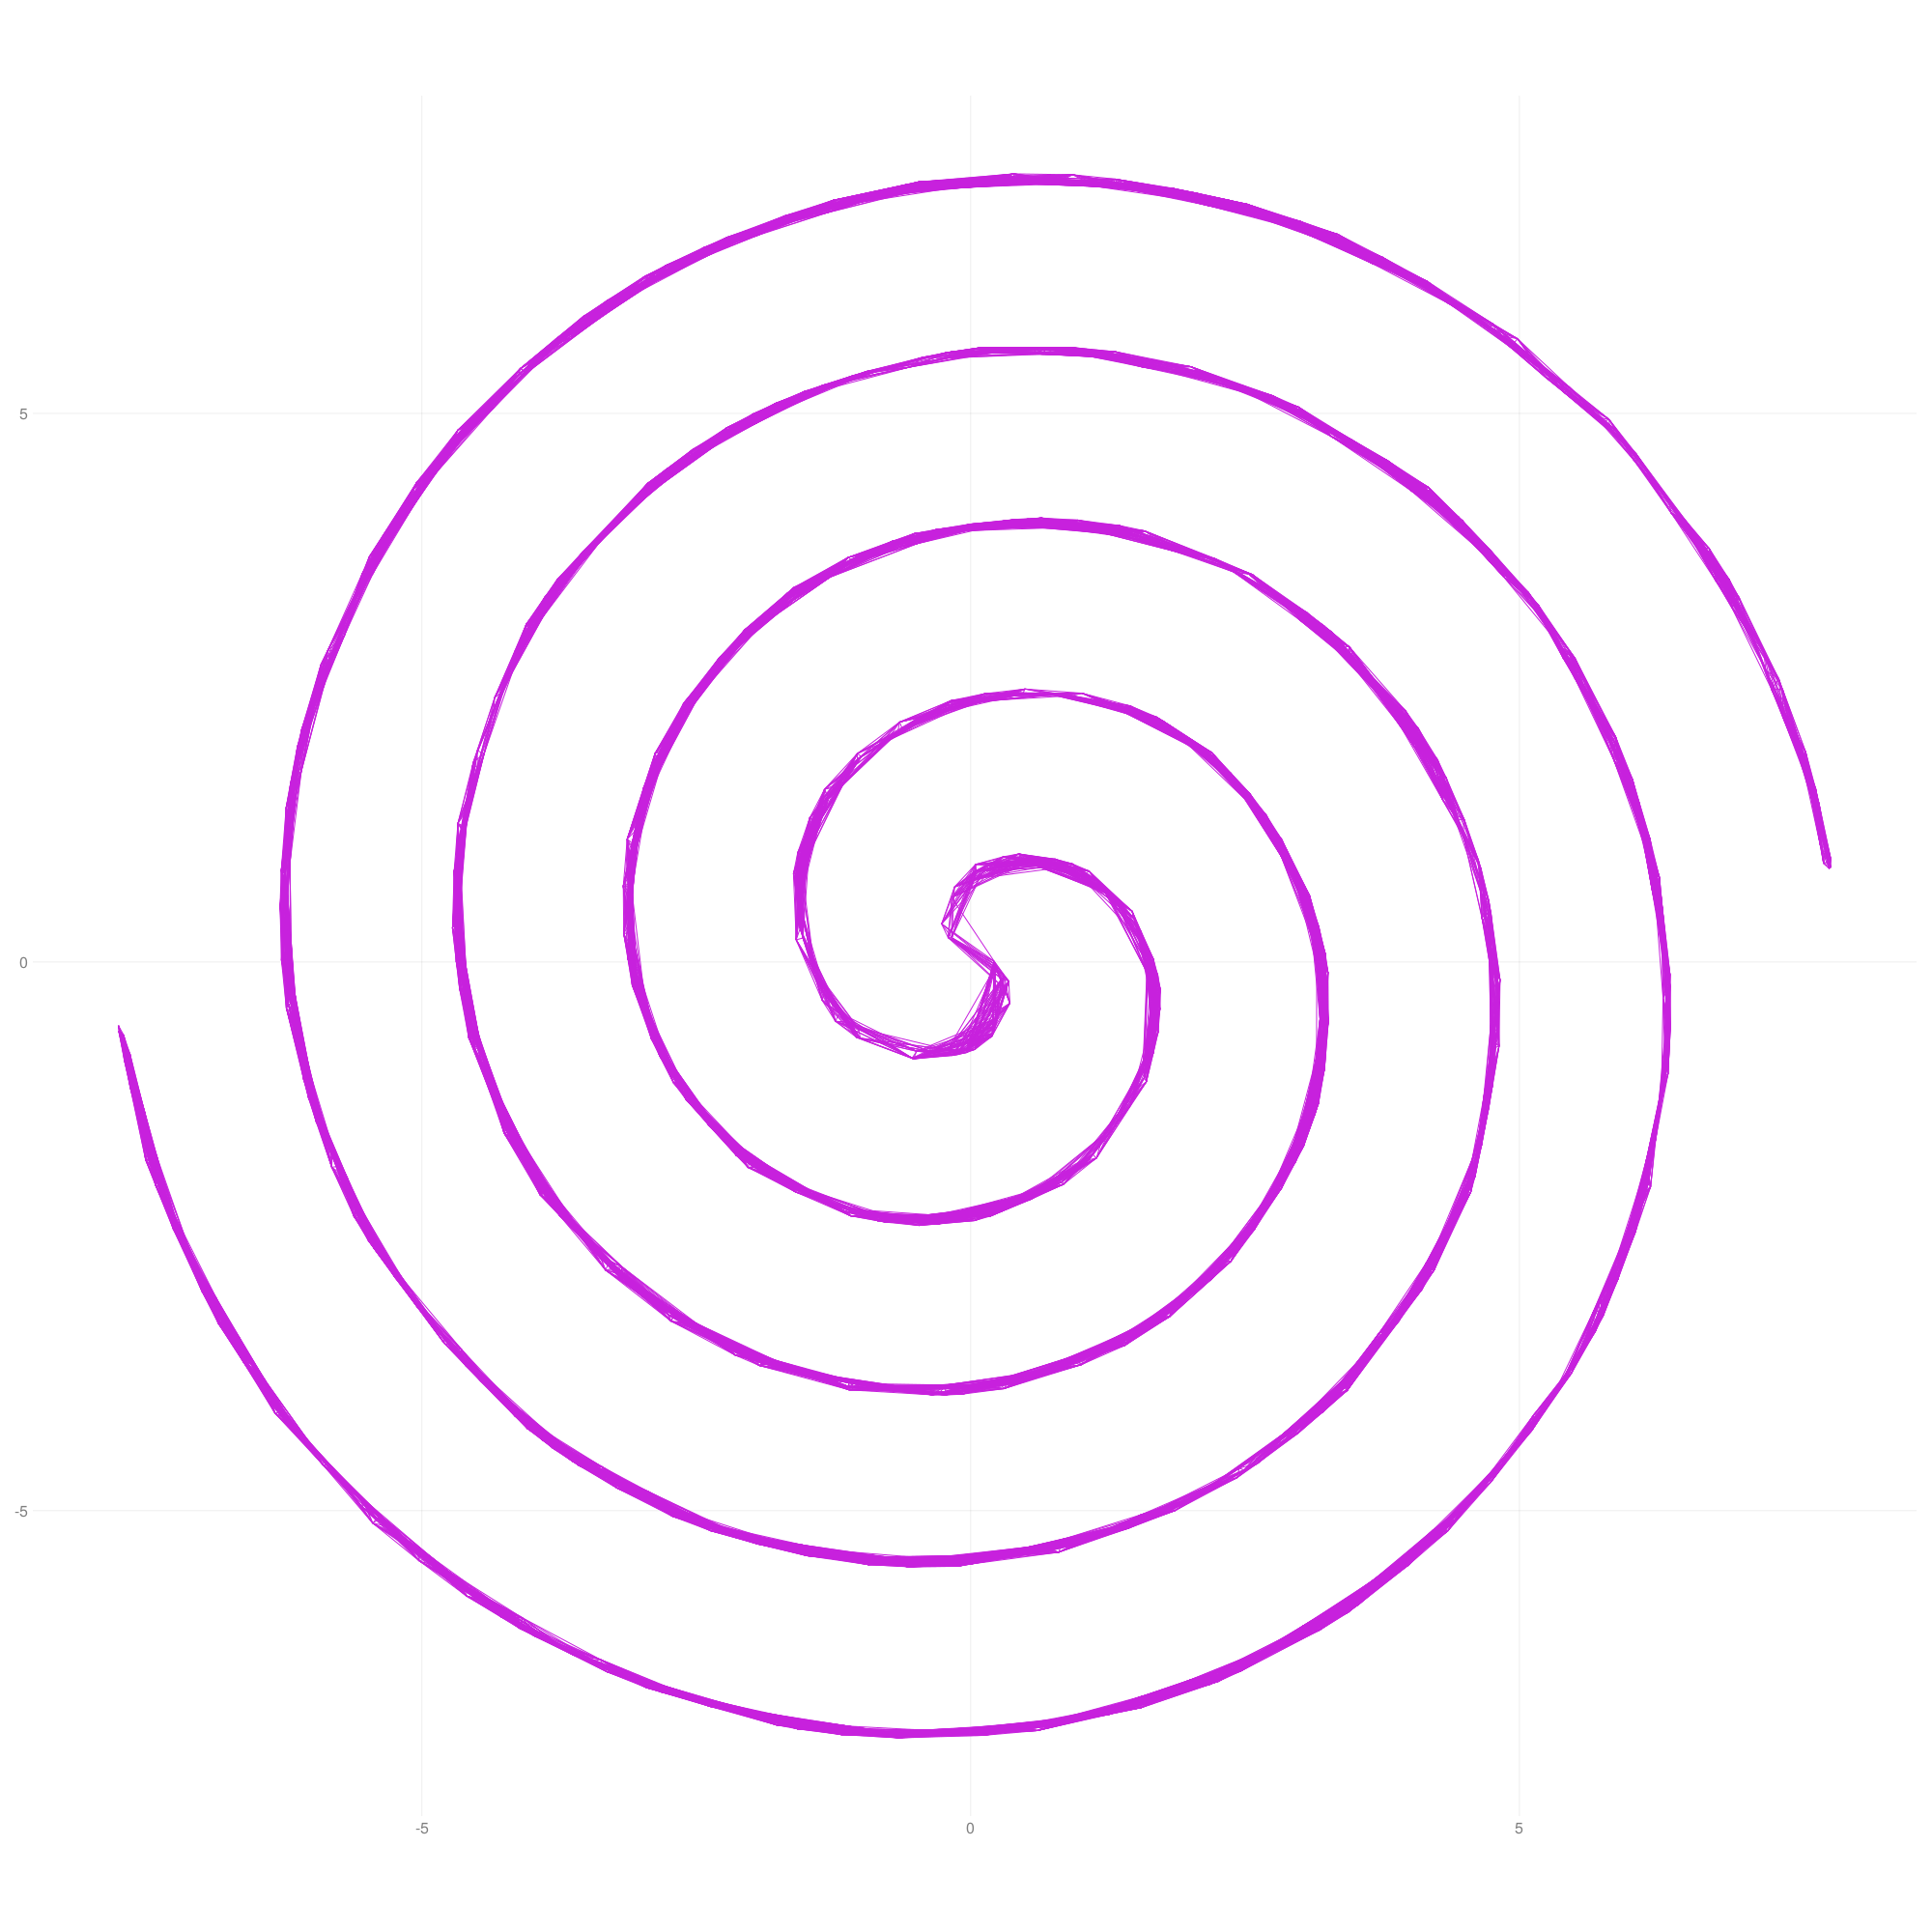
\includegraphics[width=0.5\linewidth]{fig/1/4.'pts_spiral'-epsilon-adjacency.png}
        \caption{$\texttt {pts\_spiral }\epsilon$ adjacency graph.}
    \end{minipage}
    % \caption*{}
\end{figure}

\subsection*{1.5. Implementing Spectral Method}
The \textbf{graph Laplacian} is a symmetric positive semi-definite matrix that encodes various graph properties. It is computed through an adjacency matrix and it associated weight matrix. It can be easily computed using a provided function.\\\\
By running $k$-means on the eigenvectors corresponding to the $k$th smallest eigenvalues of the Laplacian matrix we are considering the graph through a new representation of its coordinates.\\
In this eigenvector representation the already existing similarity traits of points get accentuated, making the $k$-means' centroids find their ideal positions faster. We notice how the \textit{Spectral method} is generally more effective in clustering non-convex sets.\\
An important observation is how sensitive spectral clustering is to the construction of the similarity graph and the choice of its parameters $\epsilon$ and $\sigma$.\\
\begin{figure}[h!]
\begin{minted}[
frame=lines,
framesep=2mm,
]{julia}
    # ...
    K = 2
    L, D = createlaplacian(W_e);

    #   Spectral method
    lambda = eigvals(L);
    Y = eigvecs(L);
    ind = sortperm(lambda);
    Y = Y[:,ind[begin:K]]

    #   Cluster rows of eigenvector matrix of L corresponding to K smallest eigenvalues.
    R = kmeans(Y', K);
    spec_assign = R.assignments;
    # ...
\end{minted}
\caption{Julia code implementing the Spectral method.}
\end{figure}
\clearpage
\subsection*{1.6. Performing $k$-means clustering on the input points}
Implementing the basic $k$-means algorithm on the input points is rather trivial as we use the provided \verb|kmeans| function:
\begin{figure}[h!]
\begin{minted}[
frame=lines,
framesep=2mm,
]{julia}
# ...
R = kmeans(pts', K);
data_assign = R.assignments;
\end{minted}
\caption{Julia code for performing $k$-means clustering on the input points}
\end{figure}

\subsection*{\Small 1.7. Clustered datasets with $k$-means and spectral clustering in $K = 2$ and $K = 4$}
We run the \textit{Spectral} and $k$-means clustering algorithms for $K=2$ and $K=4$ clusters.\\
Let us plot the resulting clusters for $K=2$ [Figure \ref{fig:clustering-k2}] and $K=4$ [Figure \ref{fig:clustering-k4}] respectively.\\
One major weakness off the $k$-means algorithm that can be observed is how points that are unusually far away from the rest of the graph (i.e \textit{outliers}) influence the centroid (and therefore cluster) positioning, resulting in badly-clustered points. This effect is particularly noticeable in Figure \ref{fig:pts_outlier-kmeans-k4}. We also notice how the basic $k$-means method treats all the centroids clusters as of the same size meaning that it does not take in account for clusters of heterogeneous volume. This is particularly noticeable in graphs where there are clusters that are very different in volume.\\
All the generated plots are aggregated in the next page.
\clearpage
\begin{figure}[h!]
\begin{minipage}{1\textwidth}
    \begin{minipage}{0.5\linewidth}
        \centering
        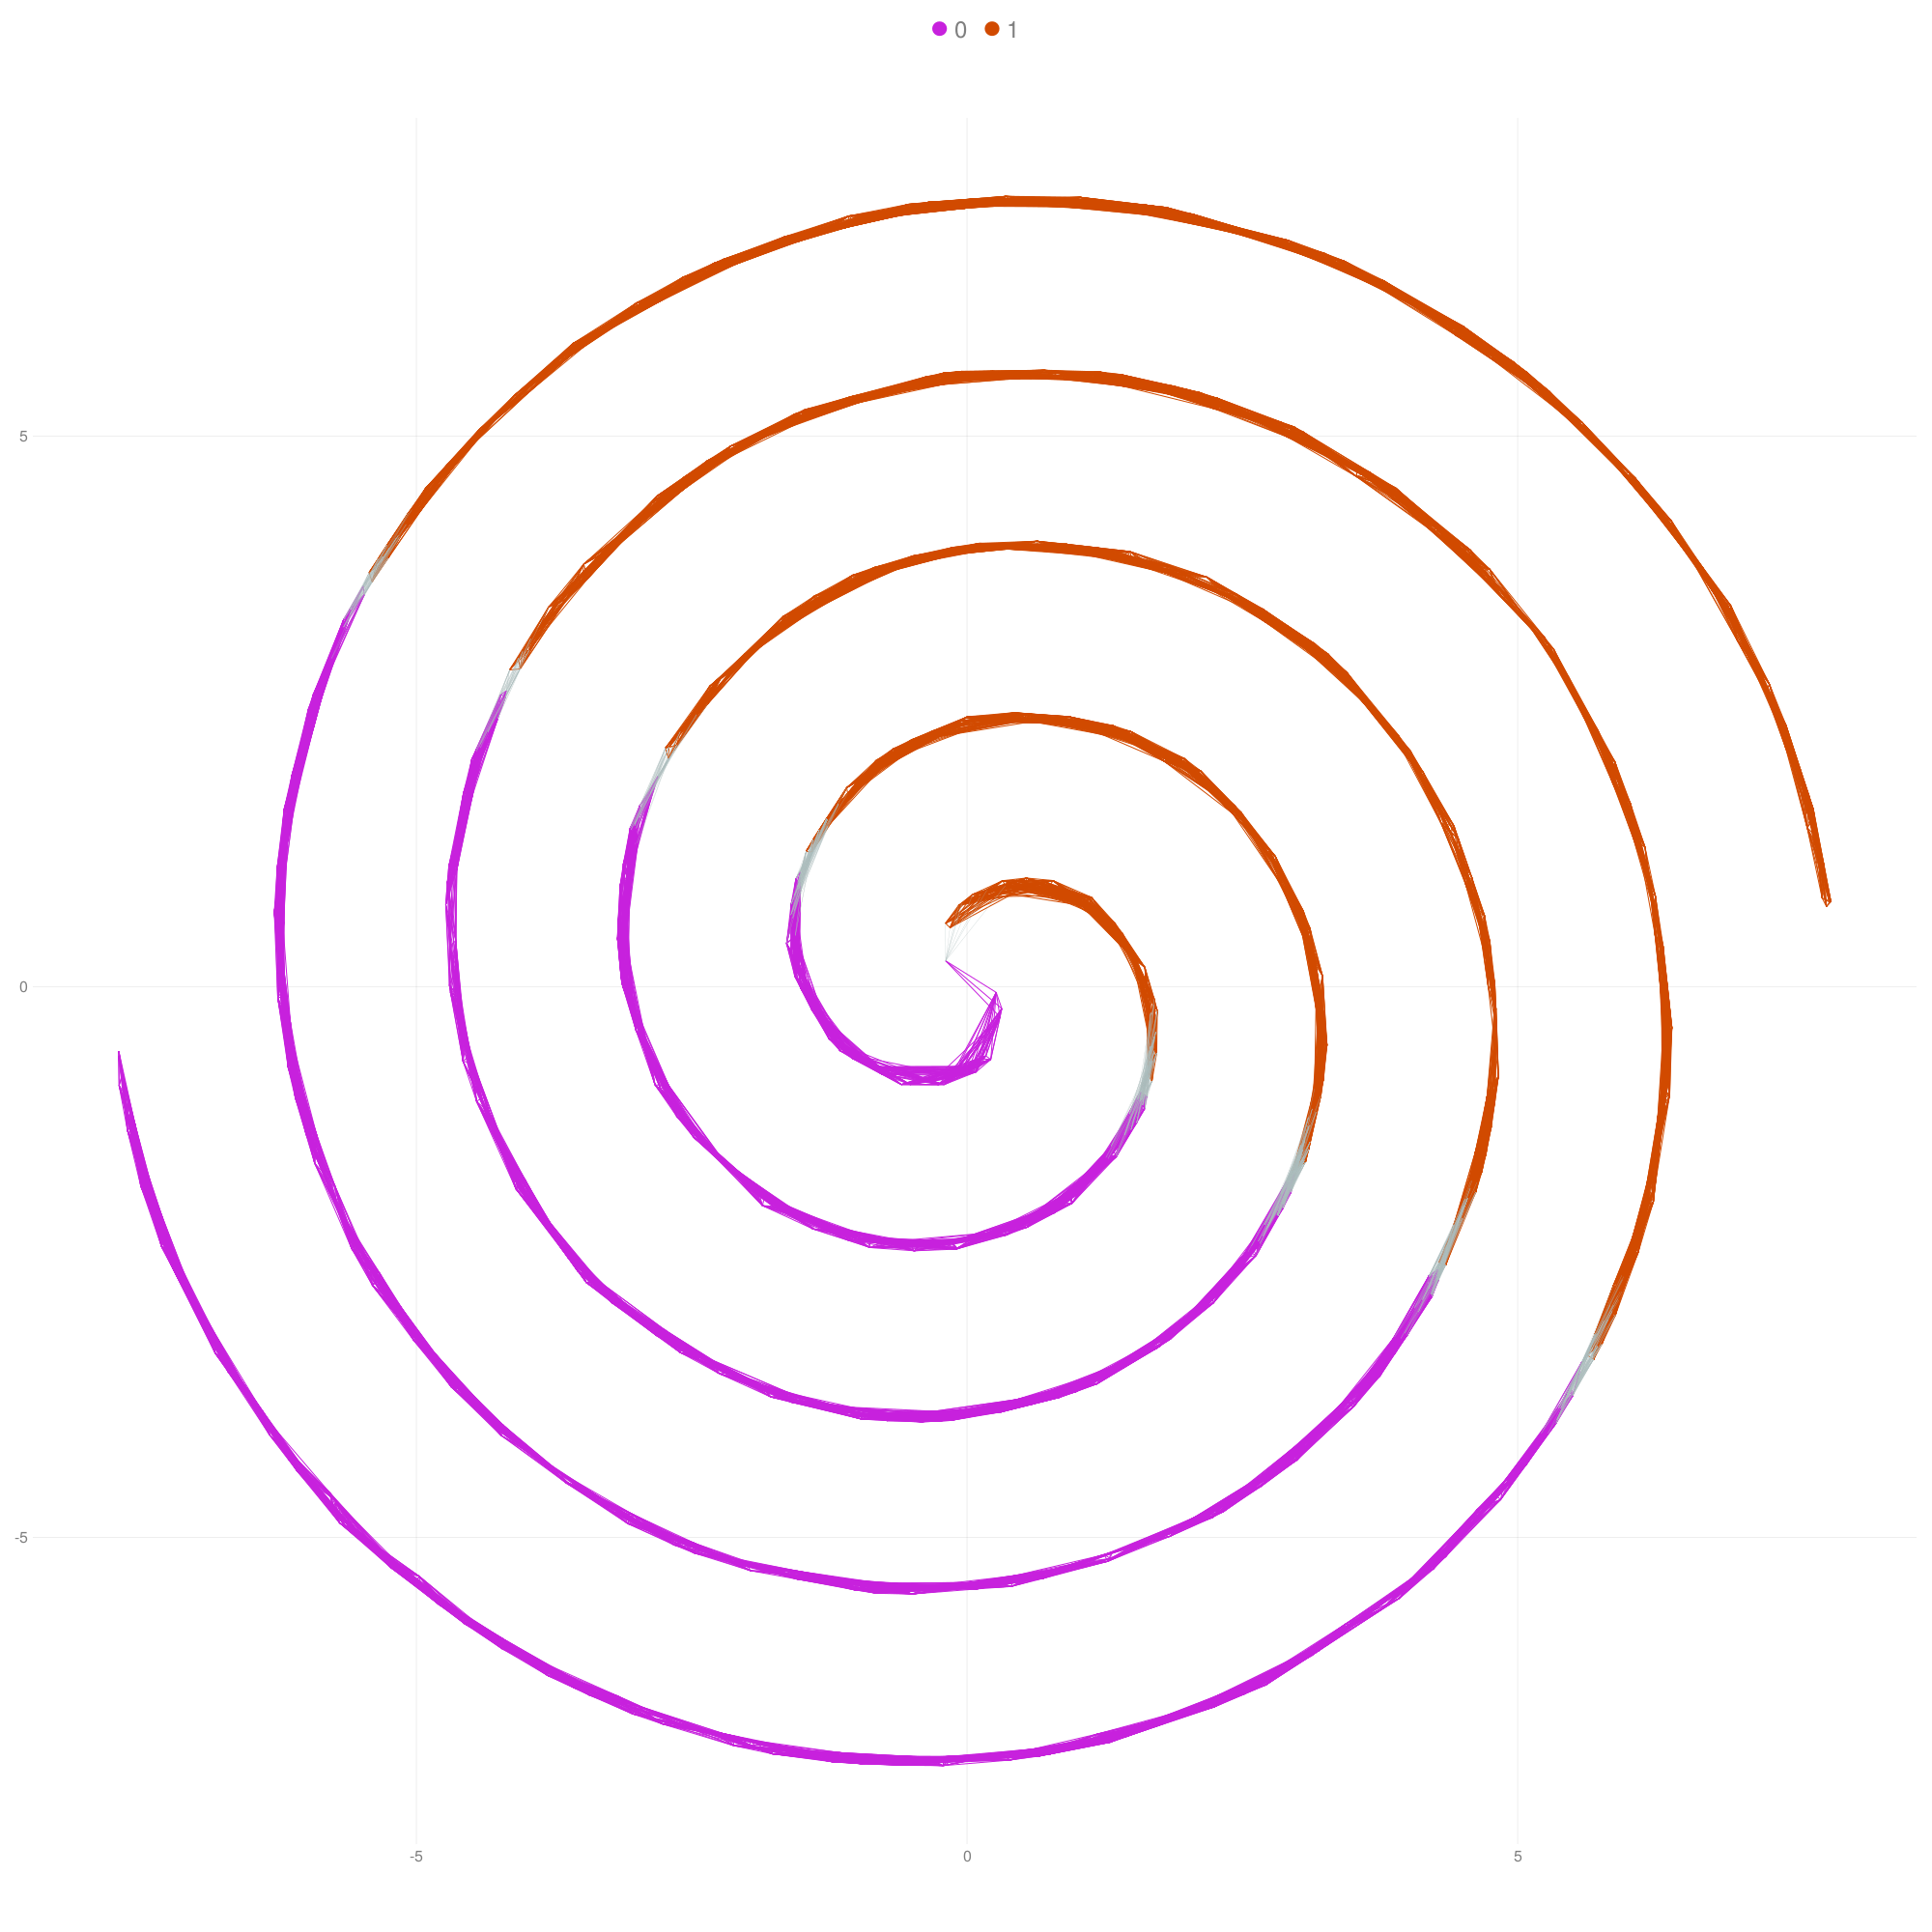
\includegraphics[height=0.4\linewidth]{fig/1/7.'pts_spiral'-K2-kmeans.png}
        \caption{$\texttt {pts\_spiral}$ $k$-means clustering.}
    \end{minipage}
    \begin{minipage}{0.5\linewidth}
        \centering
        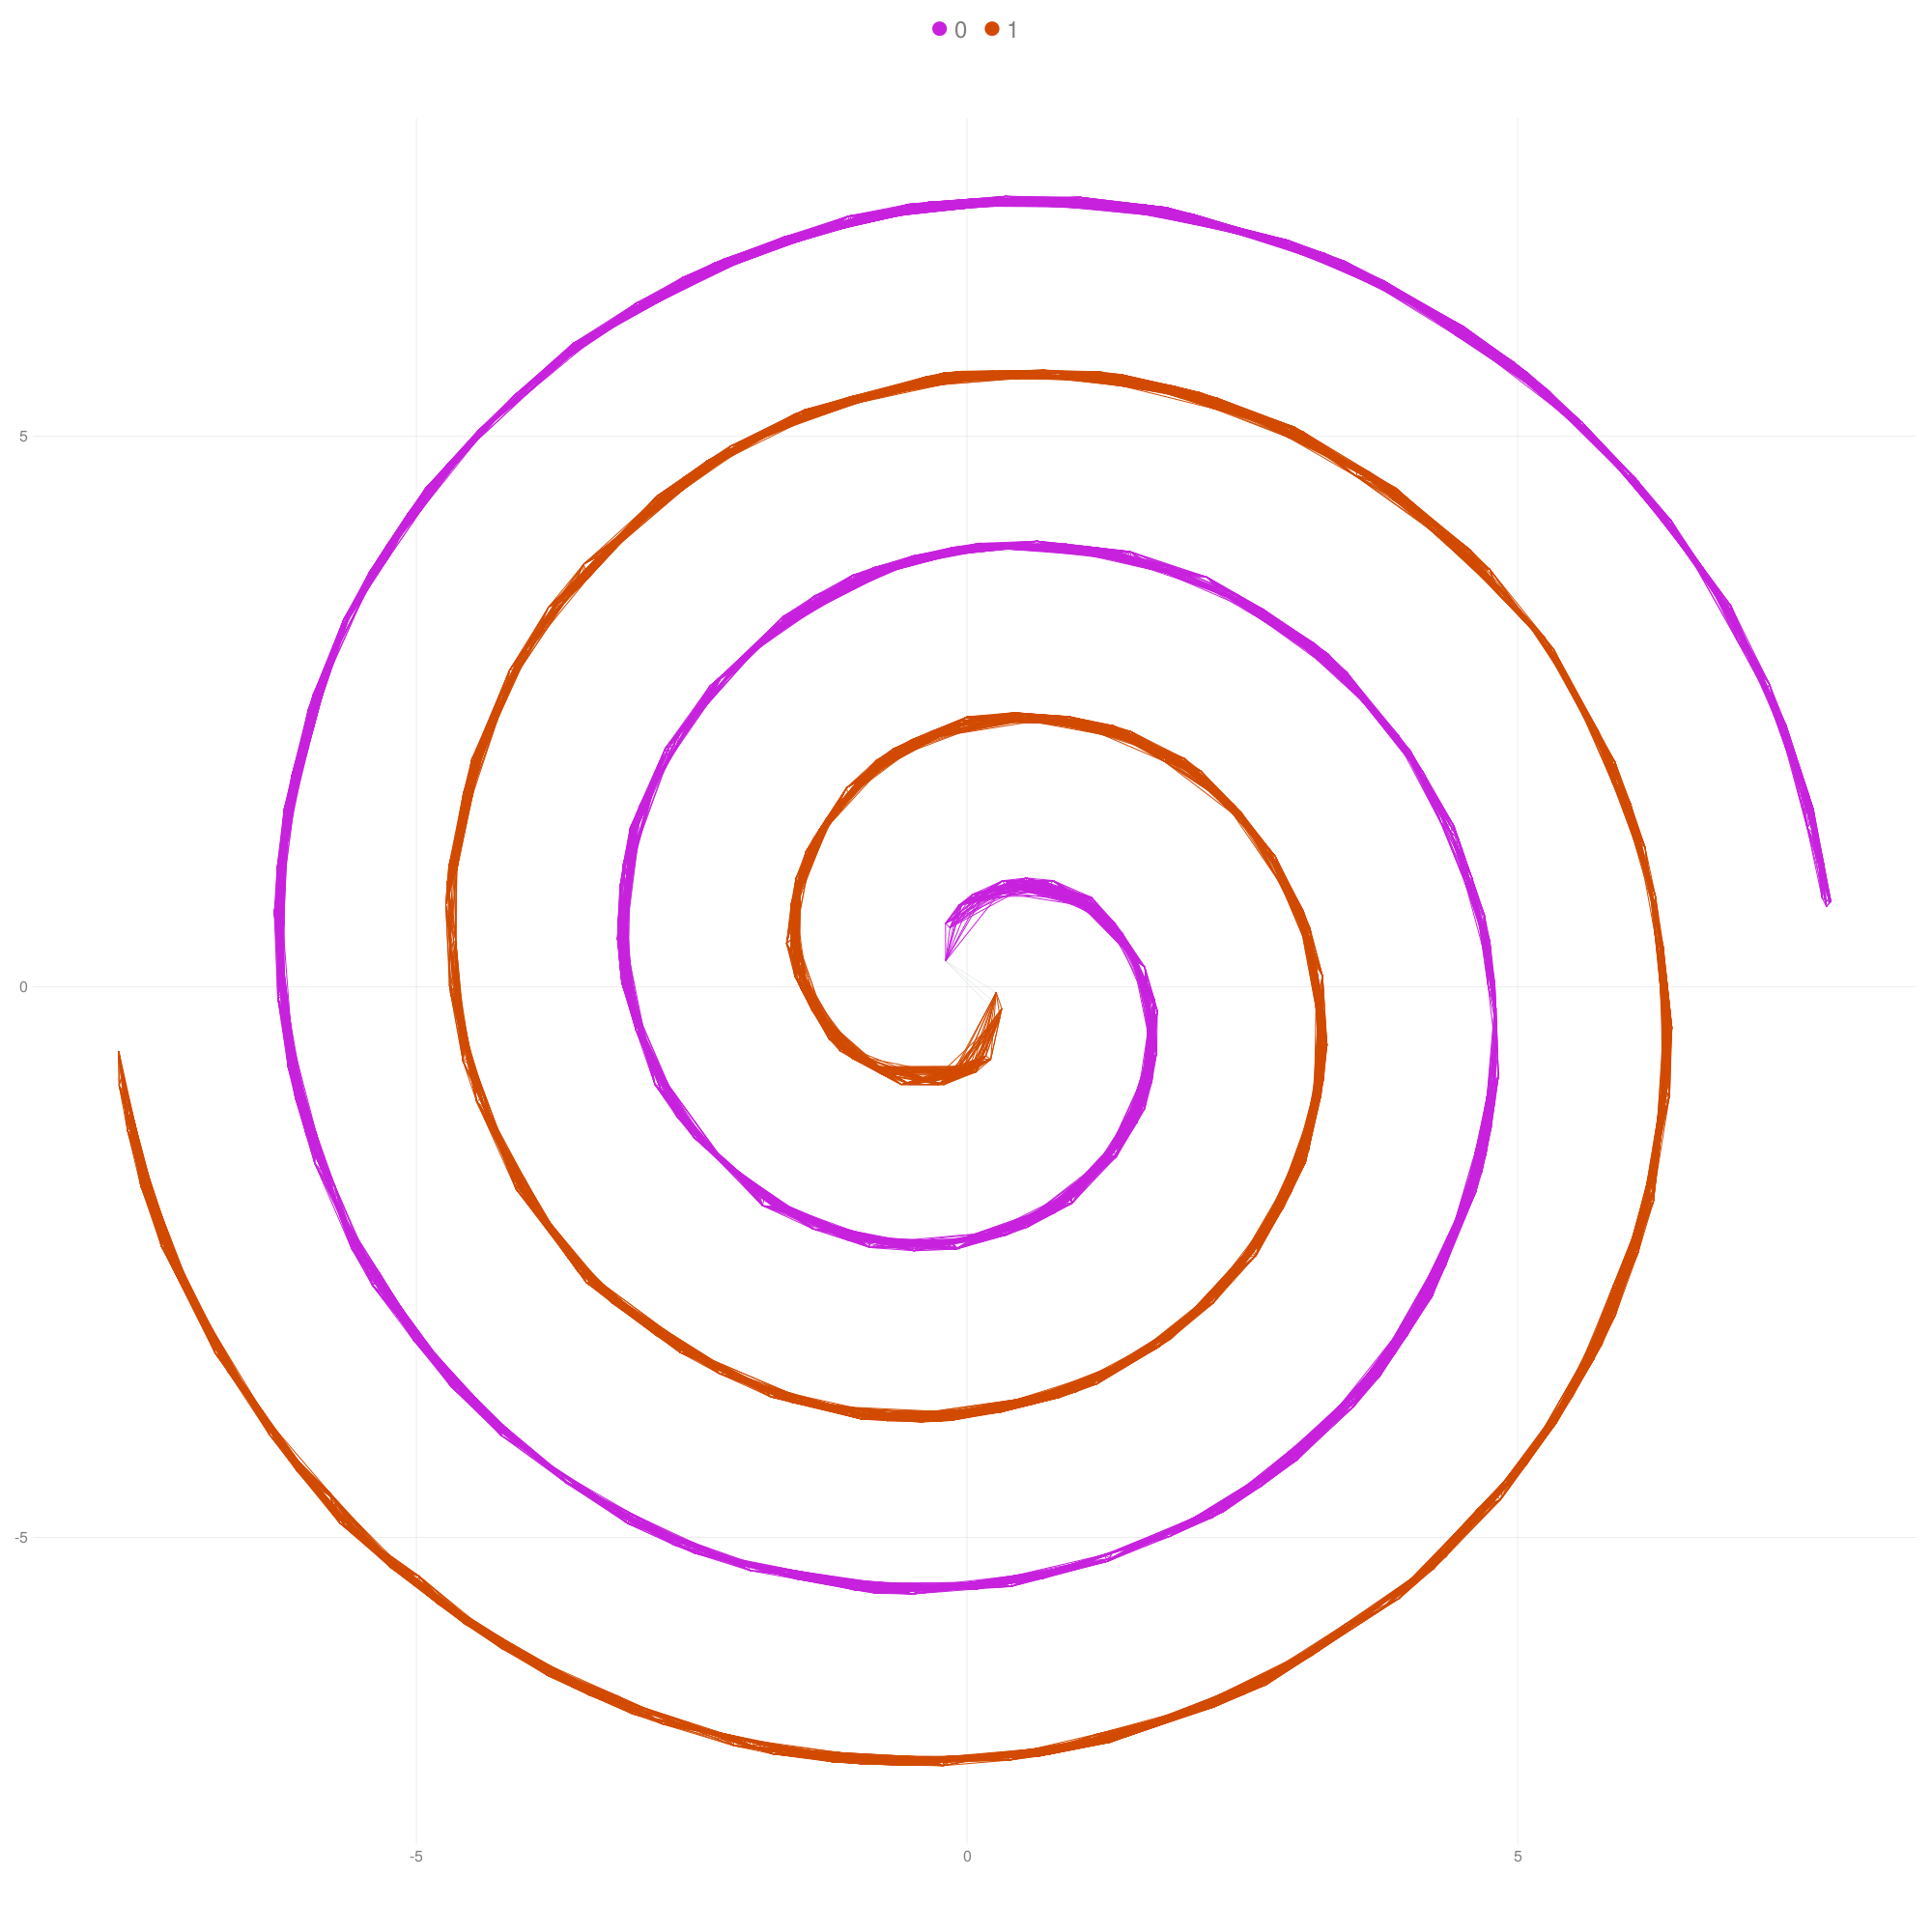
\includegraphics[height=0.4\linewidth]{fig/1/7.'pts_spiral'-K2-spectral.png}
        \caption{$\texttt {pts\_spiral}$ spectral clustering.}
    \end{minipage}
    
    \begin{minipage}{0.5\linewidth}
        \centering
        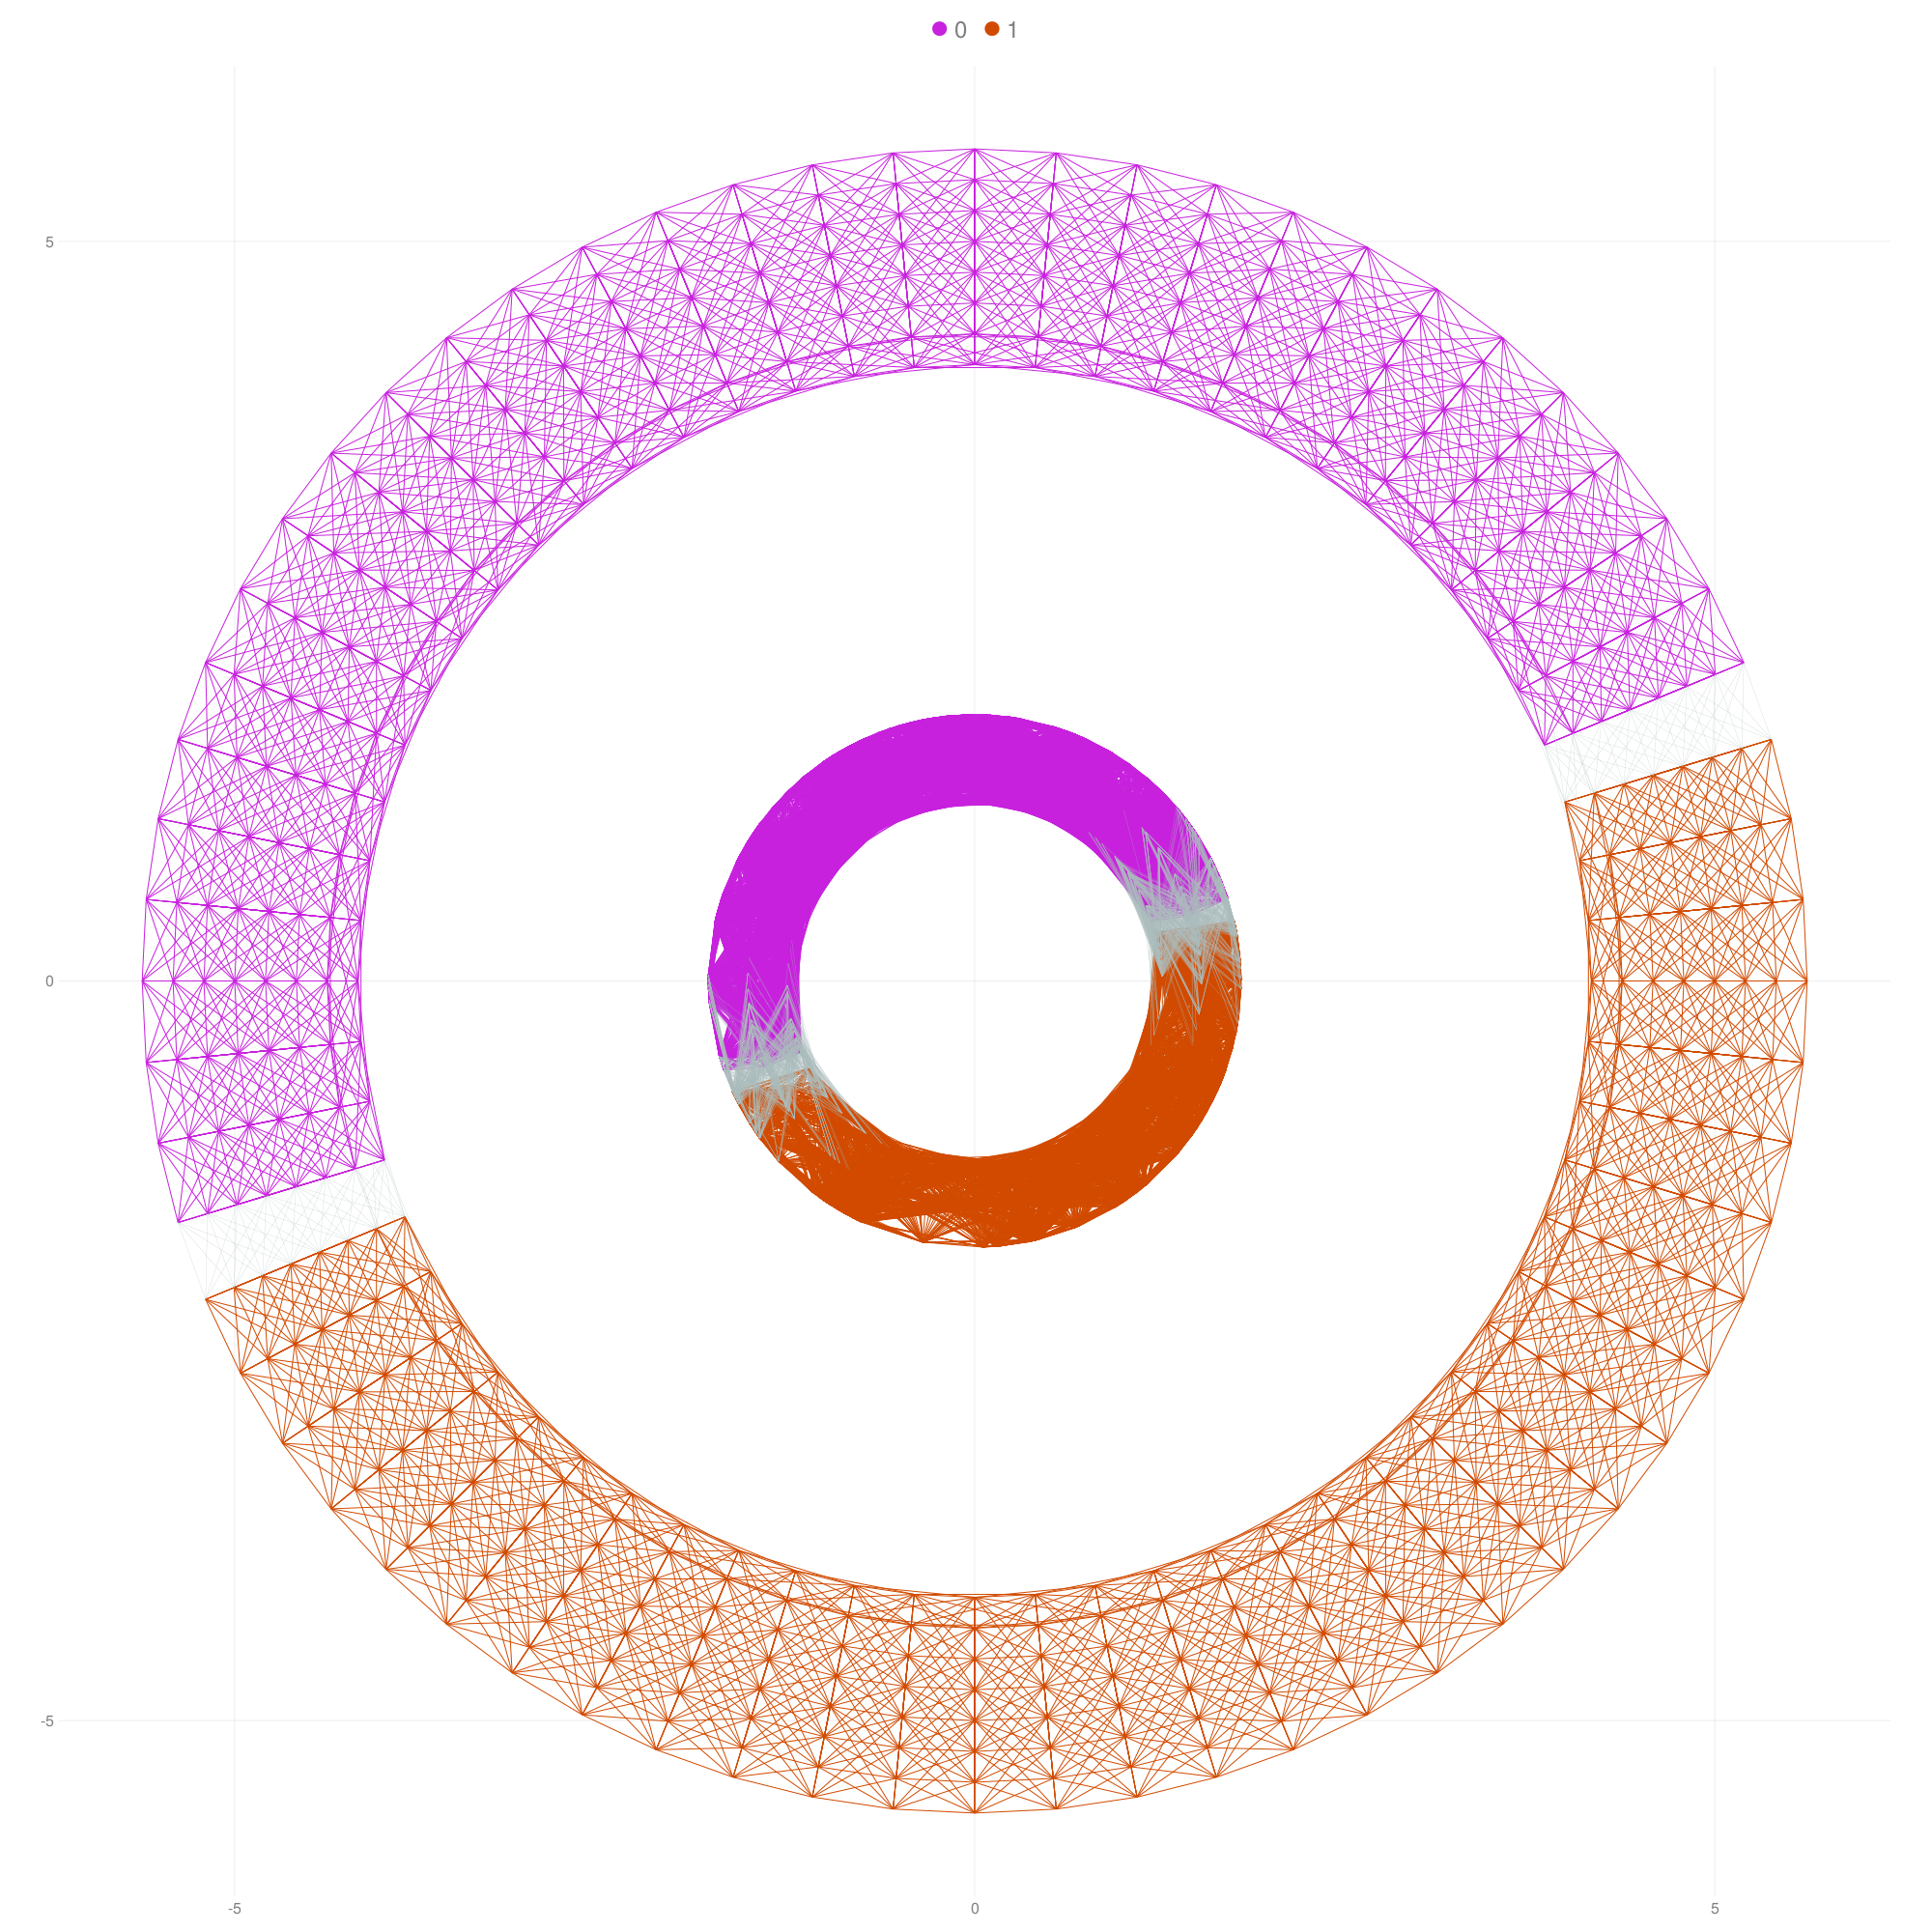
\includegraphics[height=0.4\linewidth]{fig/1/7.'pts_clusterin'-K2-kmeans.png}
        \caption{$\texttt {pts\_clusterin}$ $k$-means clustering.}
    \end{minipage}
    \begin{minipage}{0.5\linewidth}
        \centering
        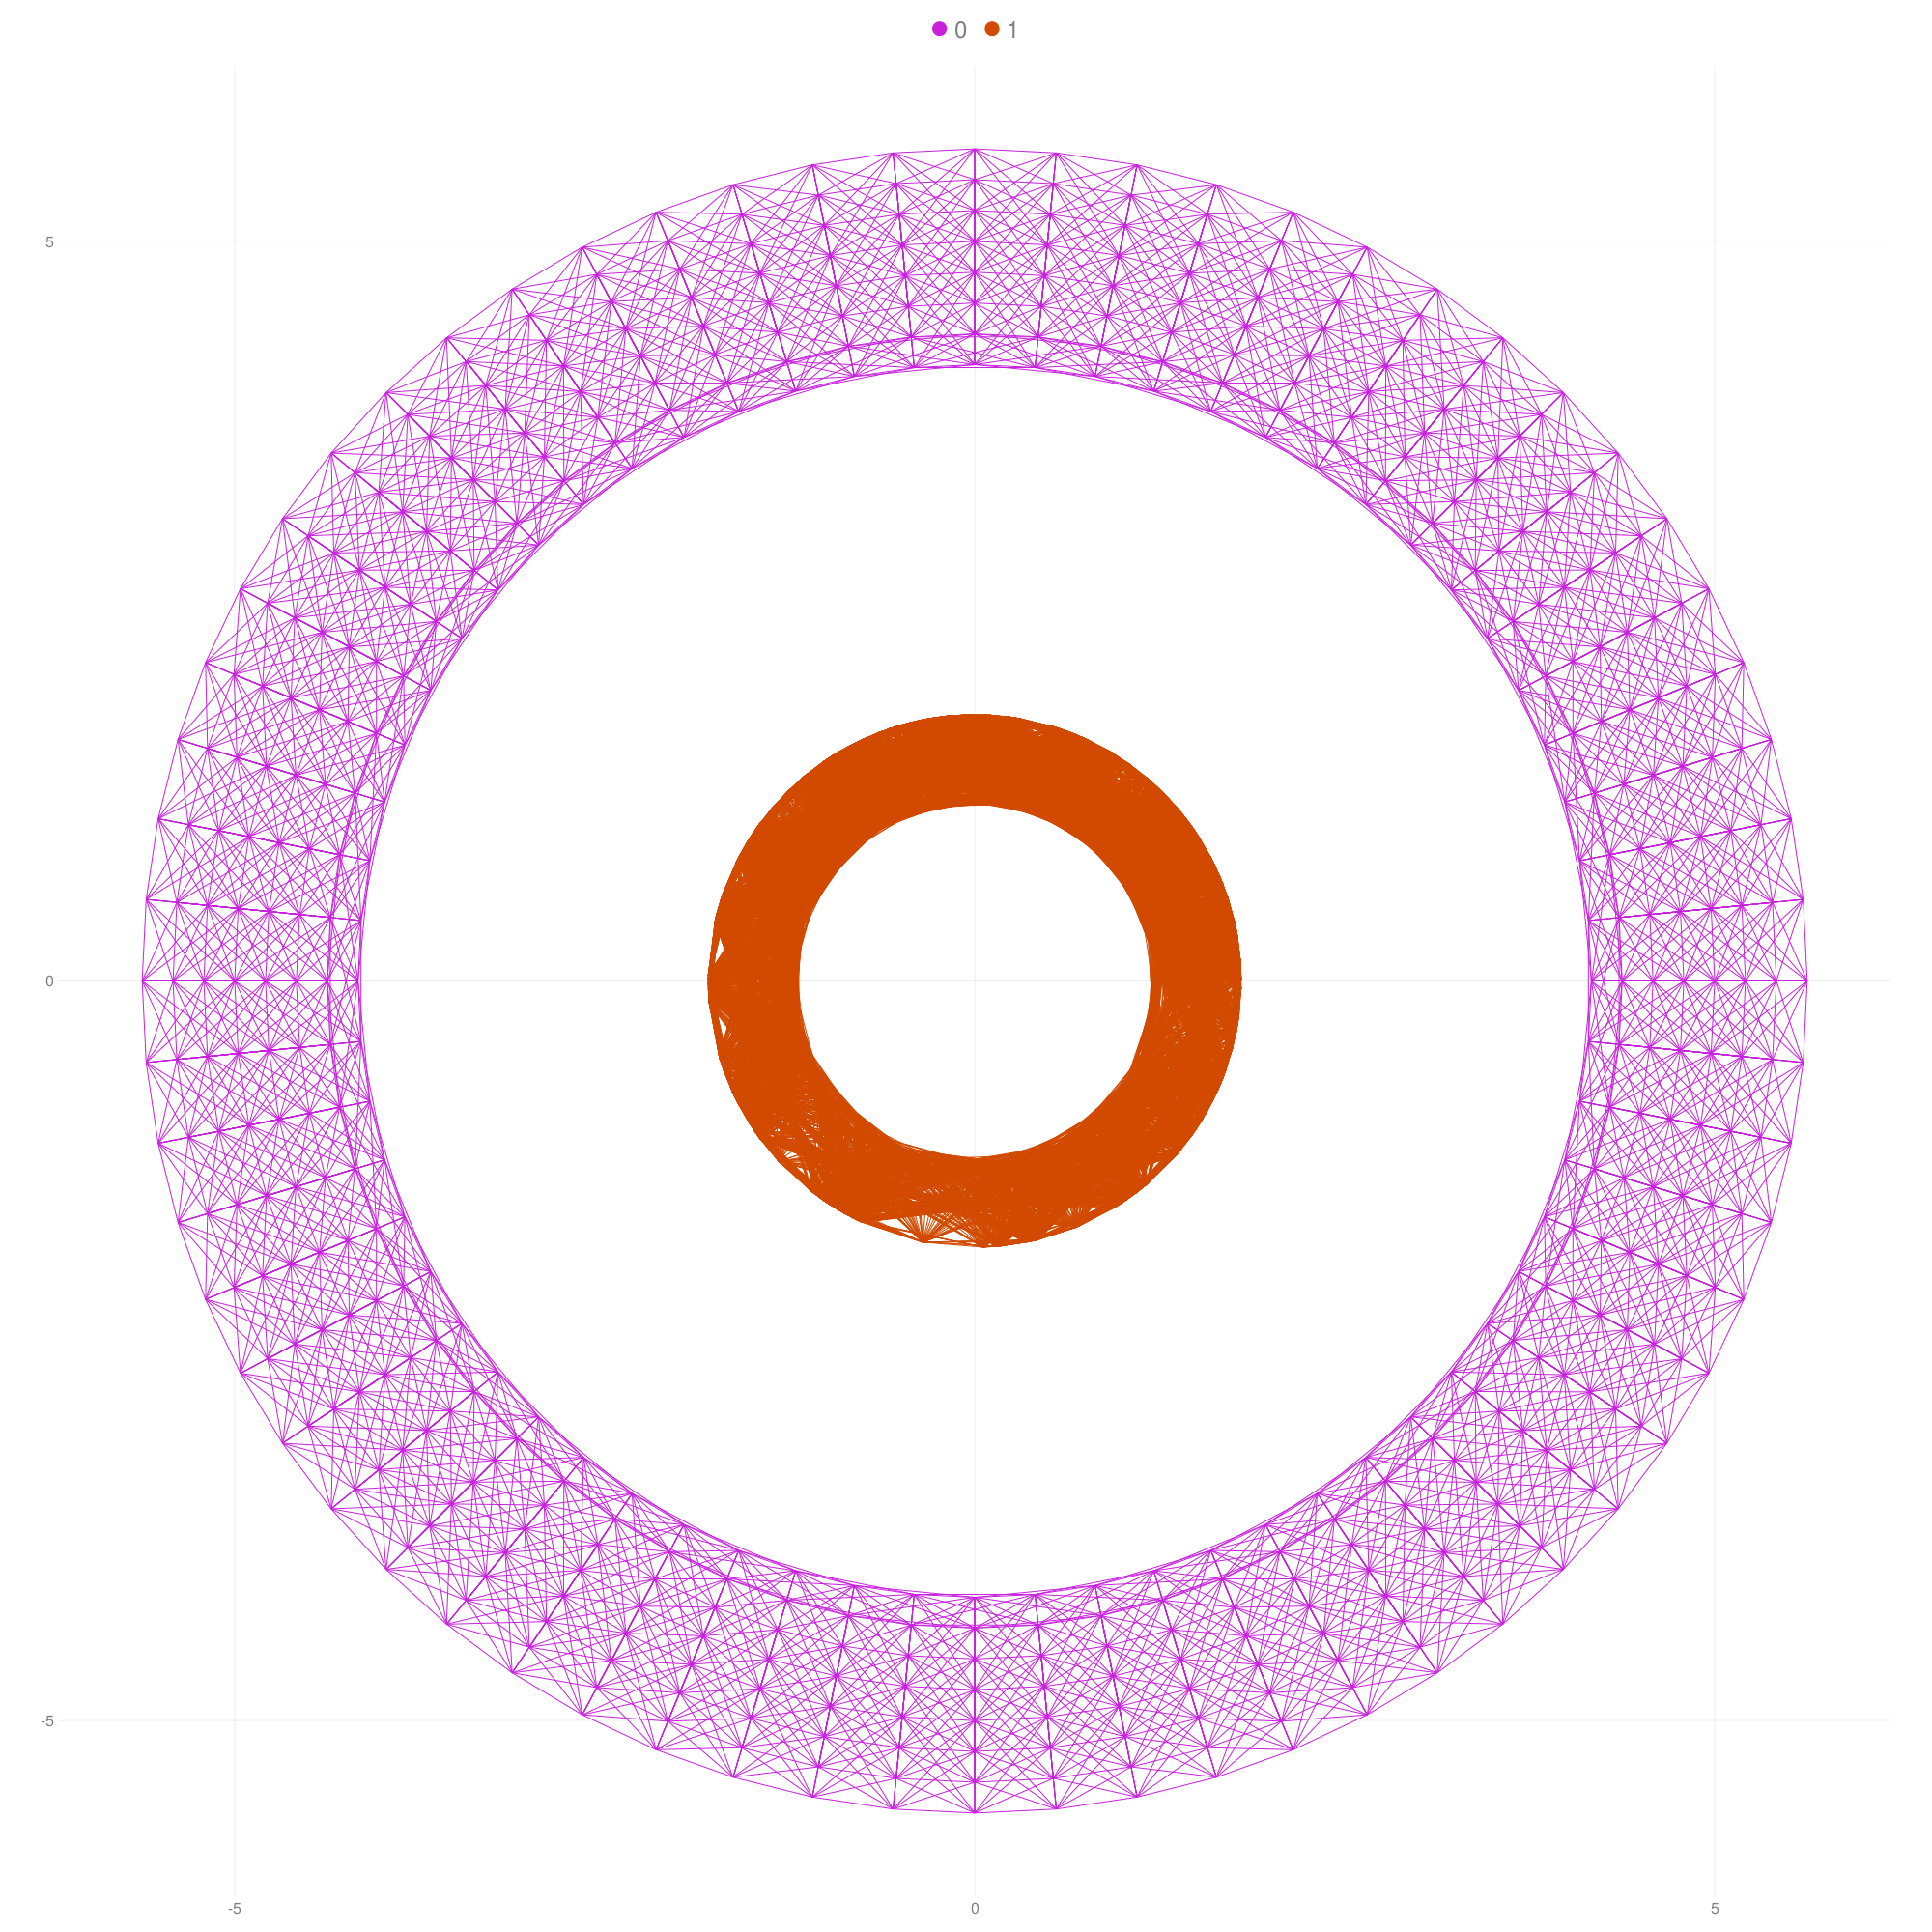
\includegraphics[height=0.4\linewidth]{fig/1/7.'pts_clusterin'-K2-spectral.png}
        \caption{$\texttt {pts\_clusterin}$ spectral clustering.}
    \end{minipage}

    \begin{minipage}{0.5\linewidth}
        \centering
        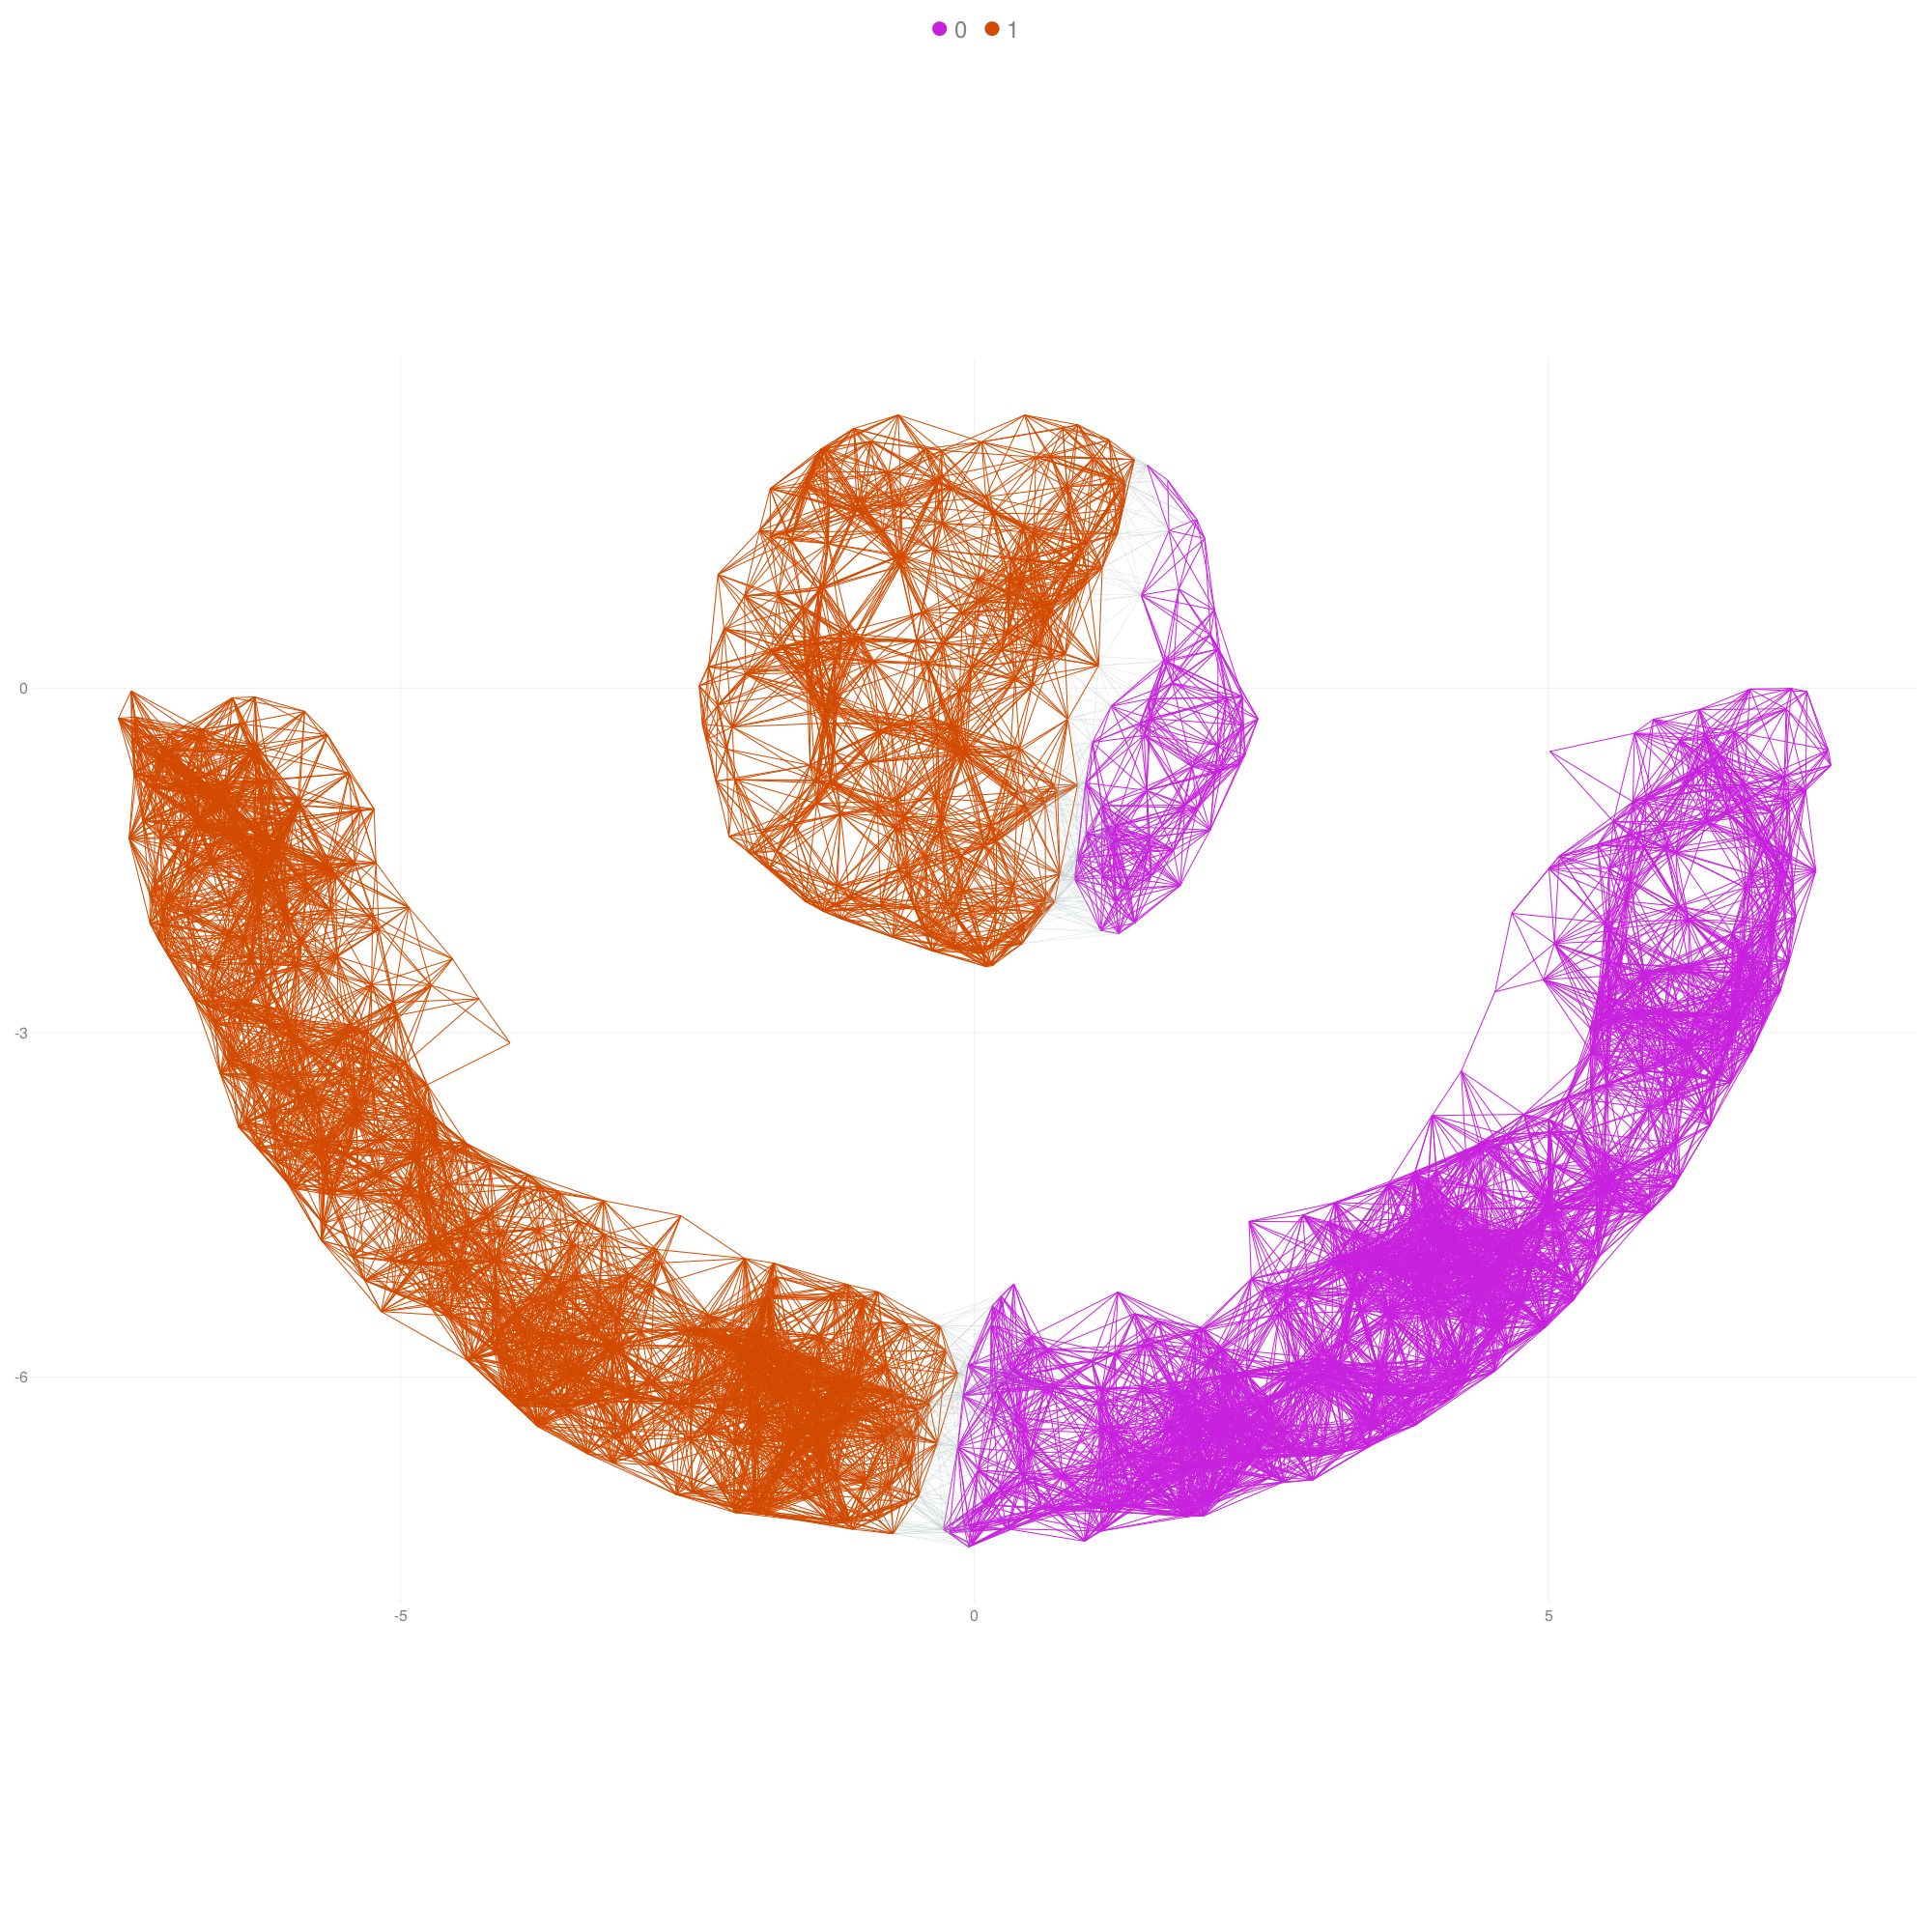
\includegraphics[height=0.4\linewidth]{fig/1/7.'pts_moon'-K2-kmeans.png}
        \caption{$\texttt {pts\_spiral}$ $k$-means clustering.}
    \end{minipage}
    \begin{minipage}{0.5\linewidth}
        \centering
        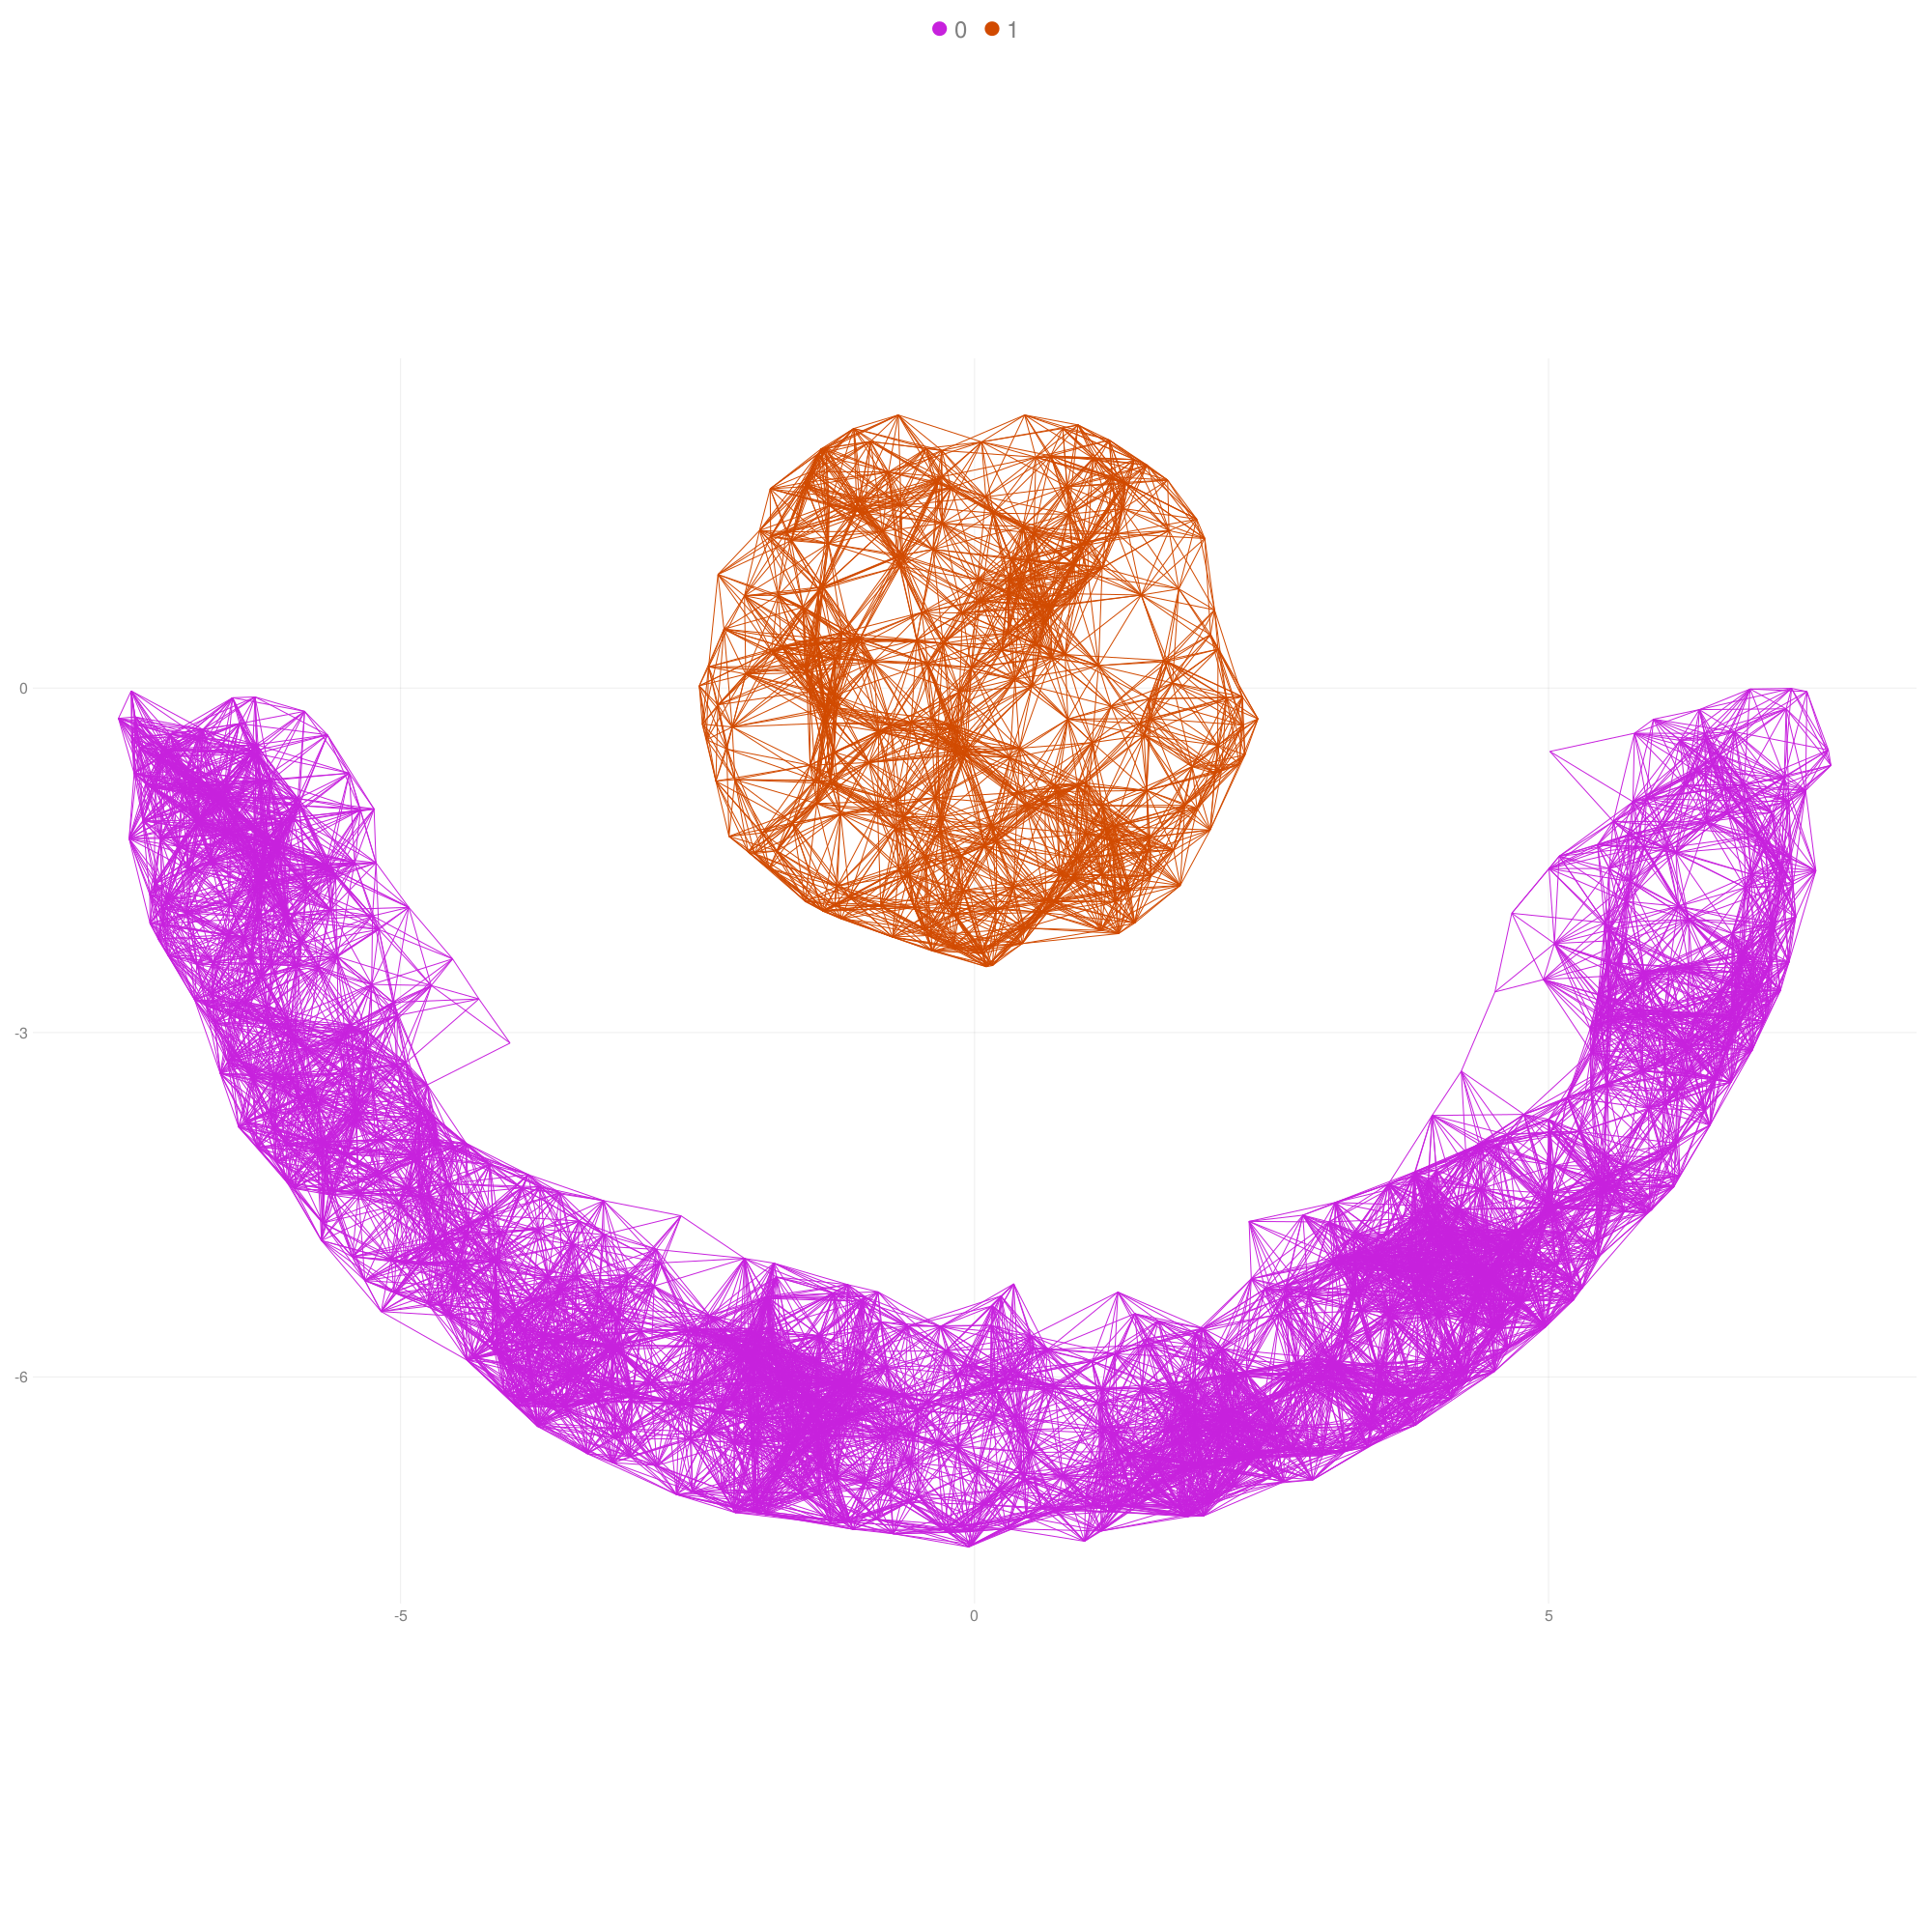
\includegraphics[height=0.4\linewidth]{fig/1/7.'pts_moon'-K2-spectral.png}
        \caption{$\texttt {pts\_spiral}$ spectral clustering.}
    \end{minipage}
\end{minipage}
    \caption{Graph clustering for $K = 2$}
        \label{fig:clustering-k2}
\end{figure}\\
\begin{figure}[h!]
\begin{minipage}{1\textwidth}
    \begin{minipage}{0.5\linewidth}
        \centering
        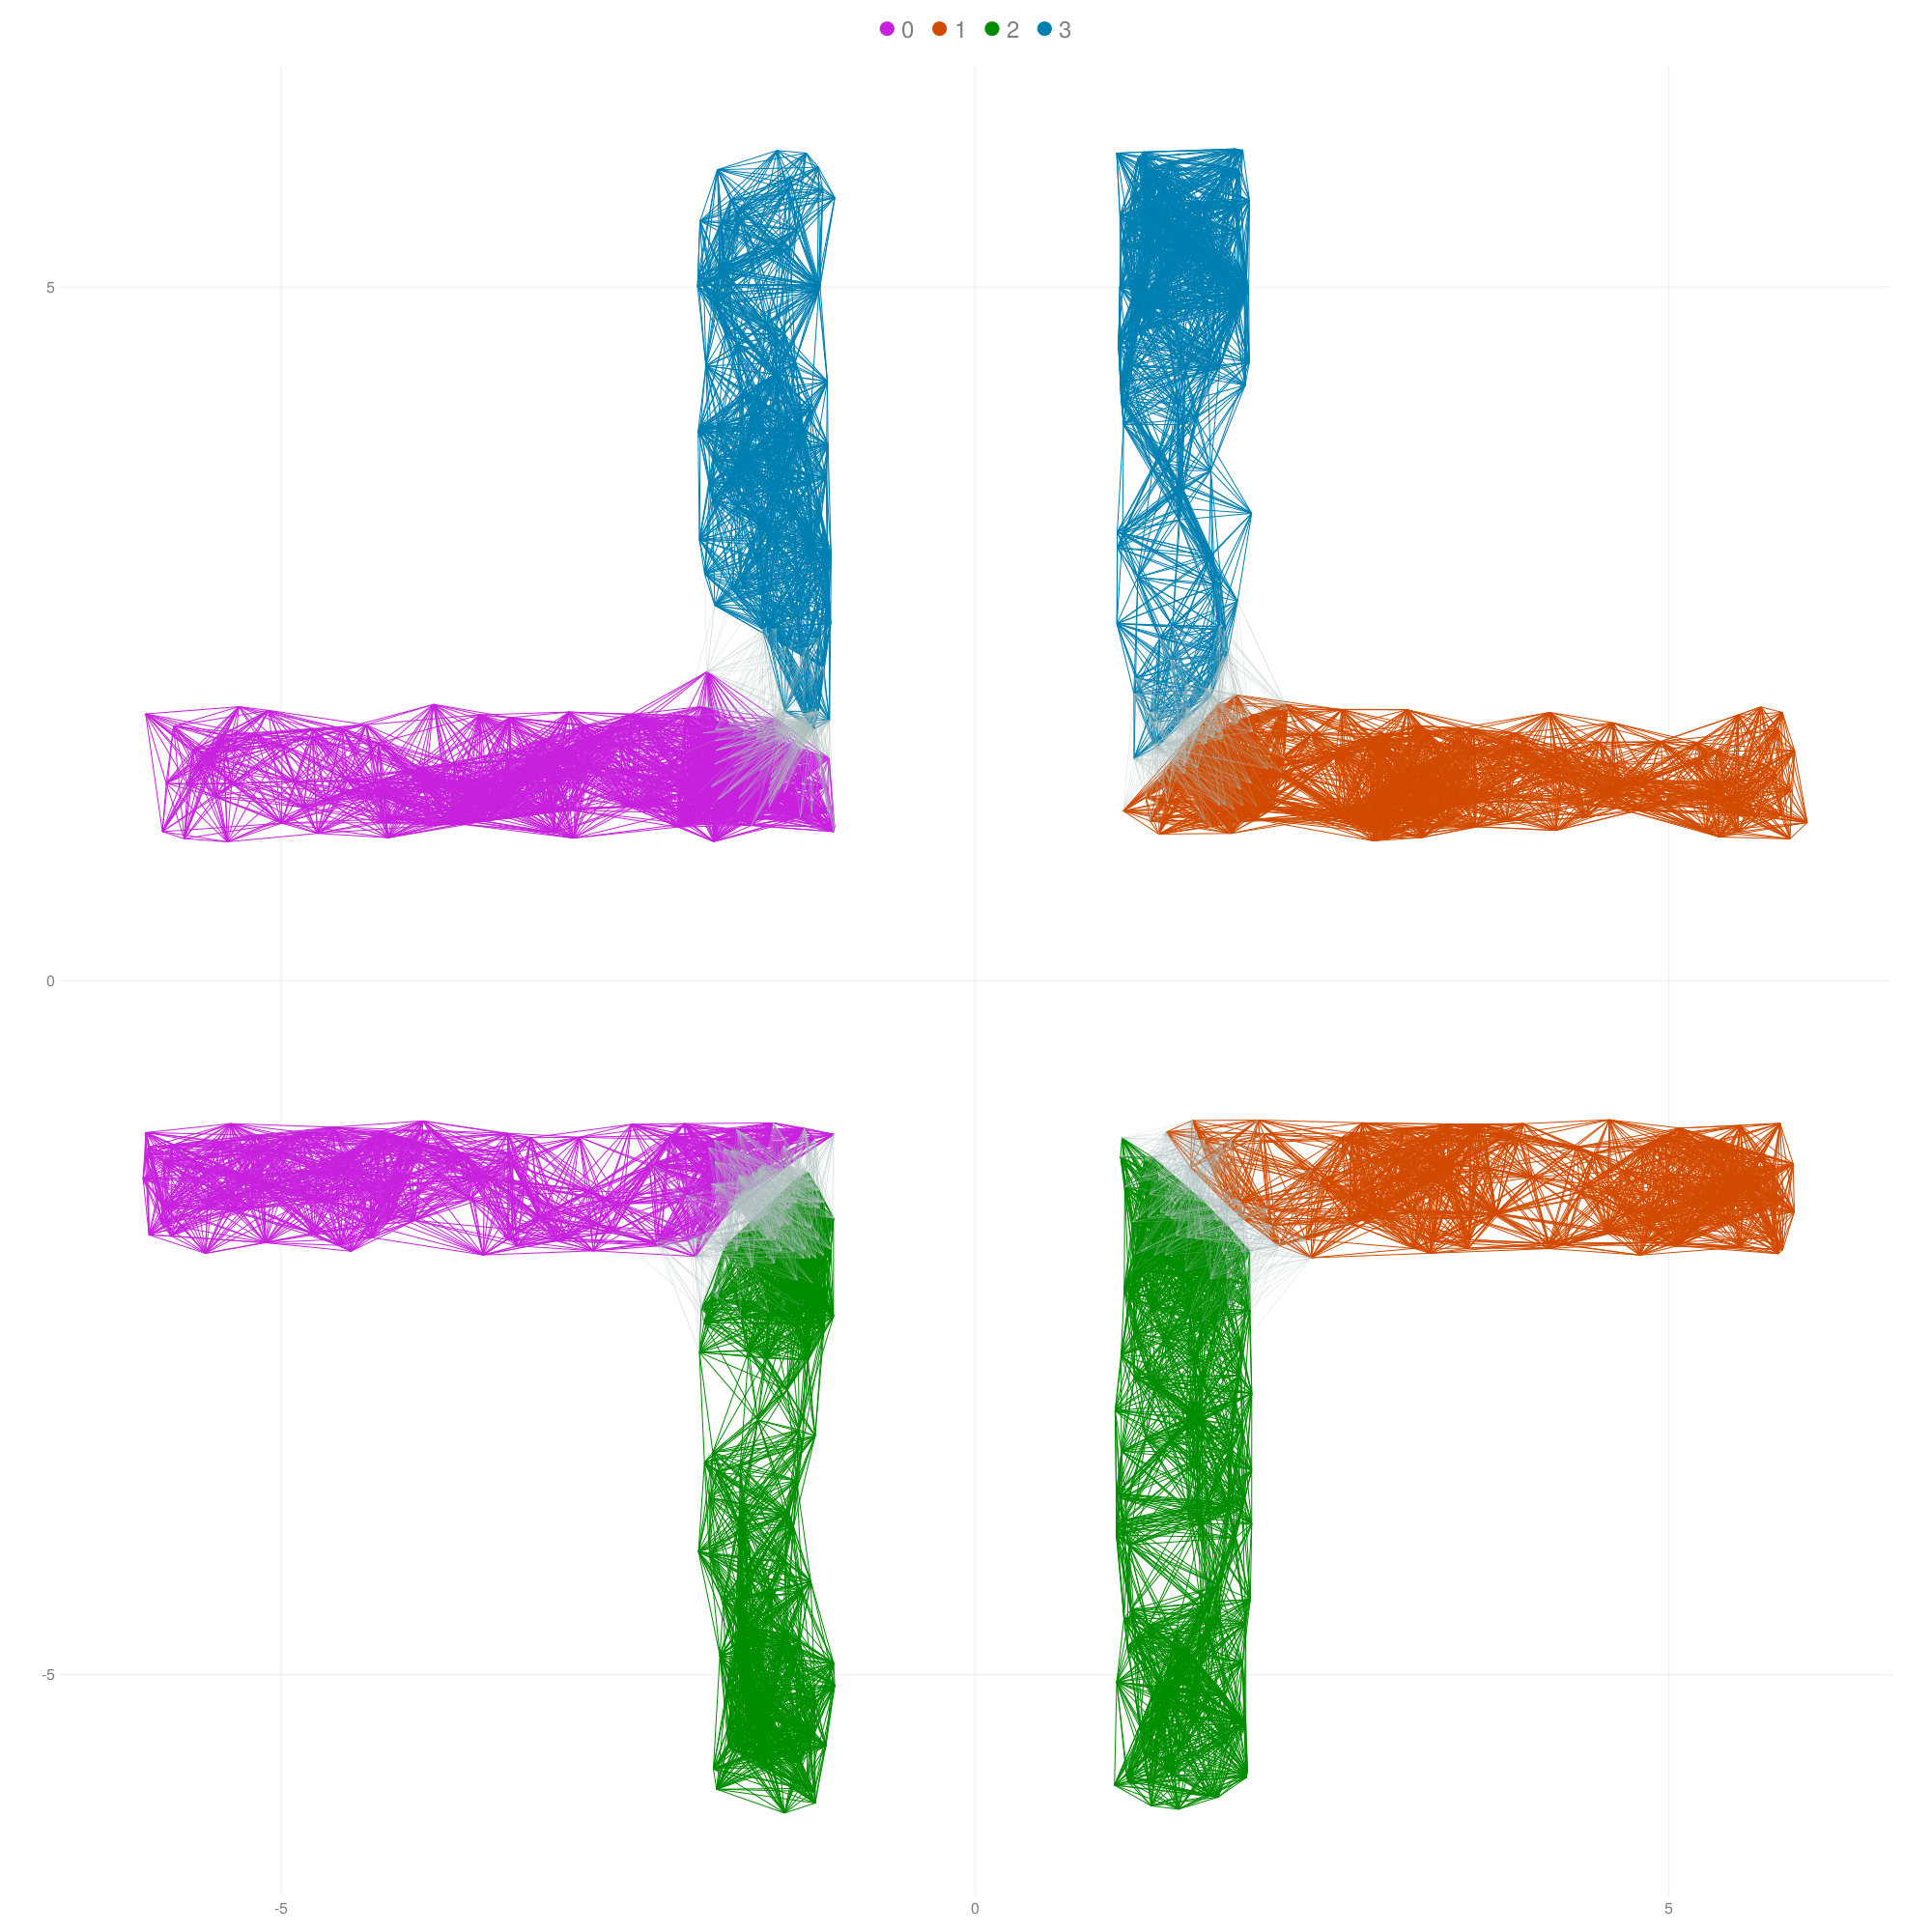
\includegraphics[height=0.4\linewidth]{fig/1/7.'pts_corn'-K4-kmeans.png}
        \caption{$\texttt {pts\_corn}$ $k$-means clustering.}
    \end{minipage}
    \begin{minipage}{0.5\linewidth}
        \centering
        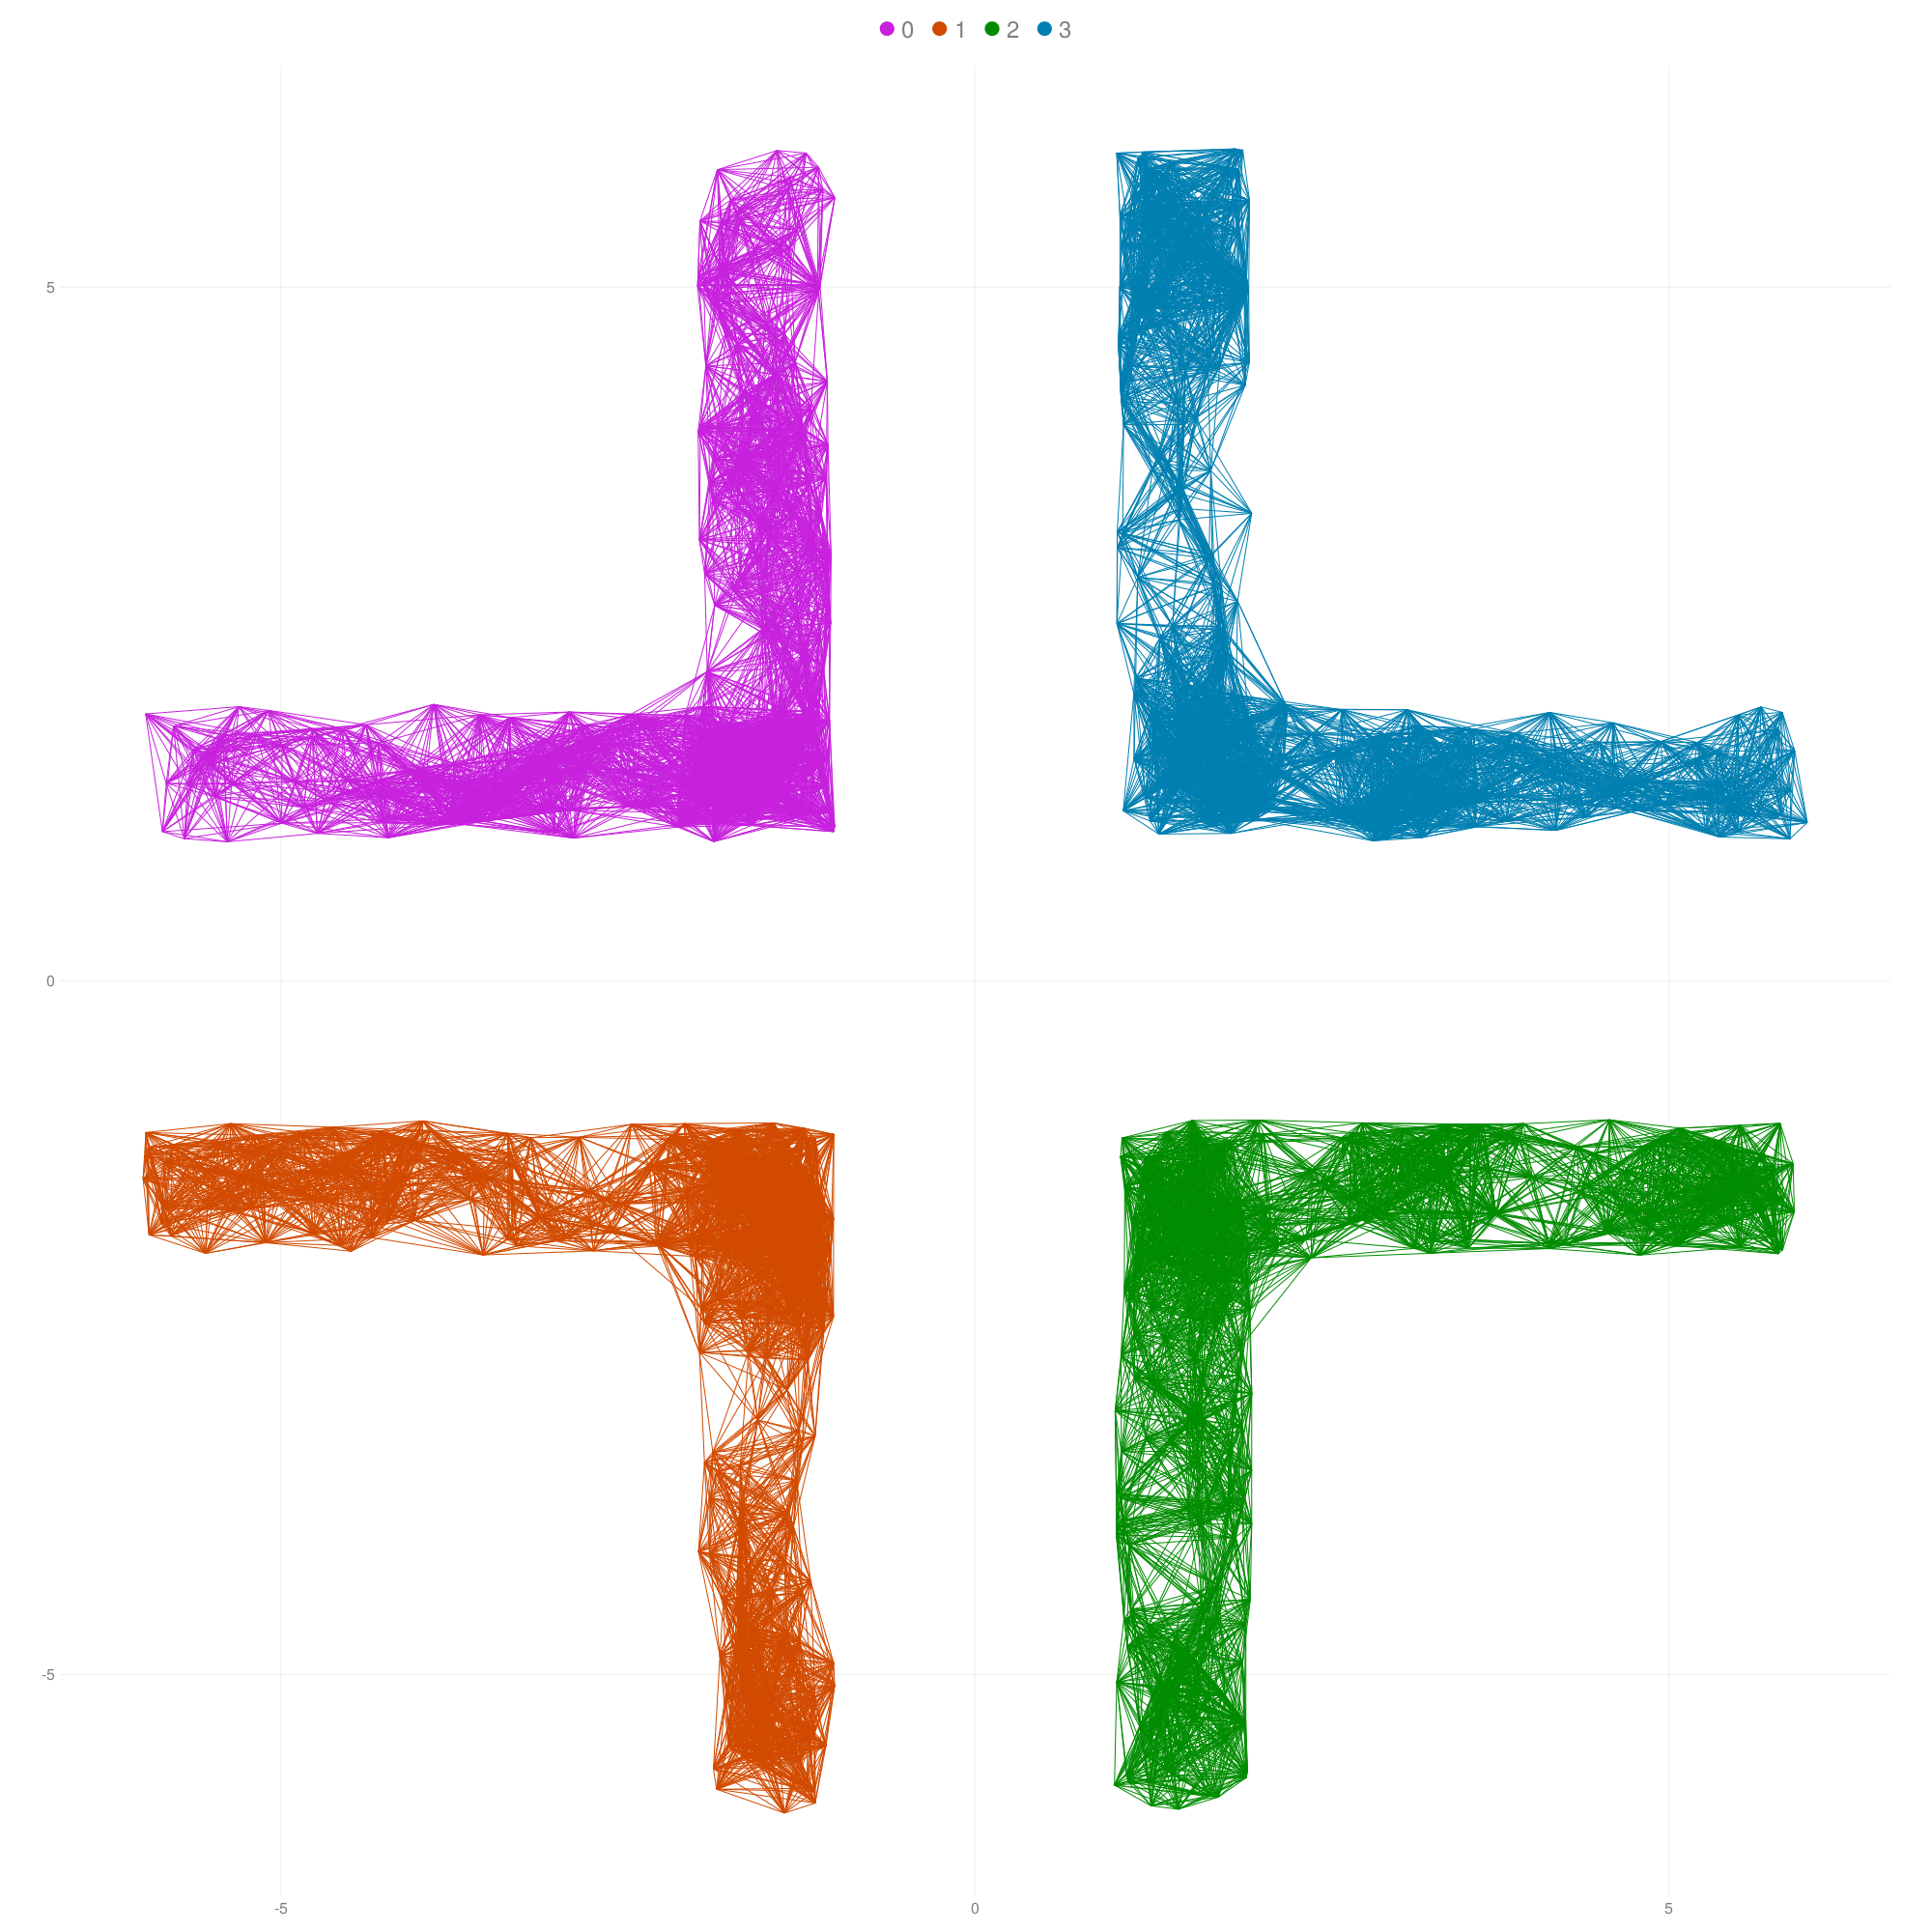
\includegraphics[height=0.4\linewidth]{fig/1/7.'pts_corn'-K4-spectral.png}
        \caption{$\texttt {pts\_corn}$ spectral clustering.}
    \end{minipage}
    
    \begin{minipage}{0.5\linewidth}
        \centering
        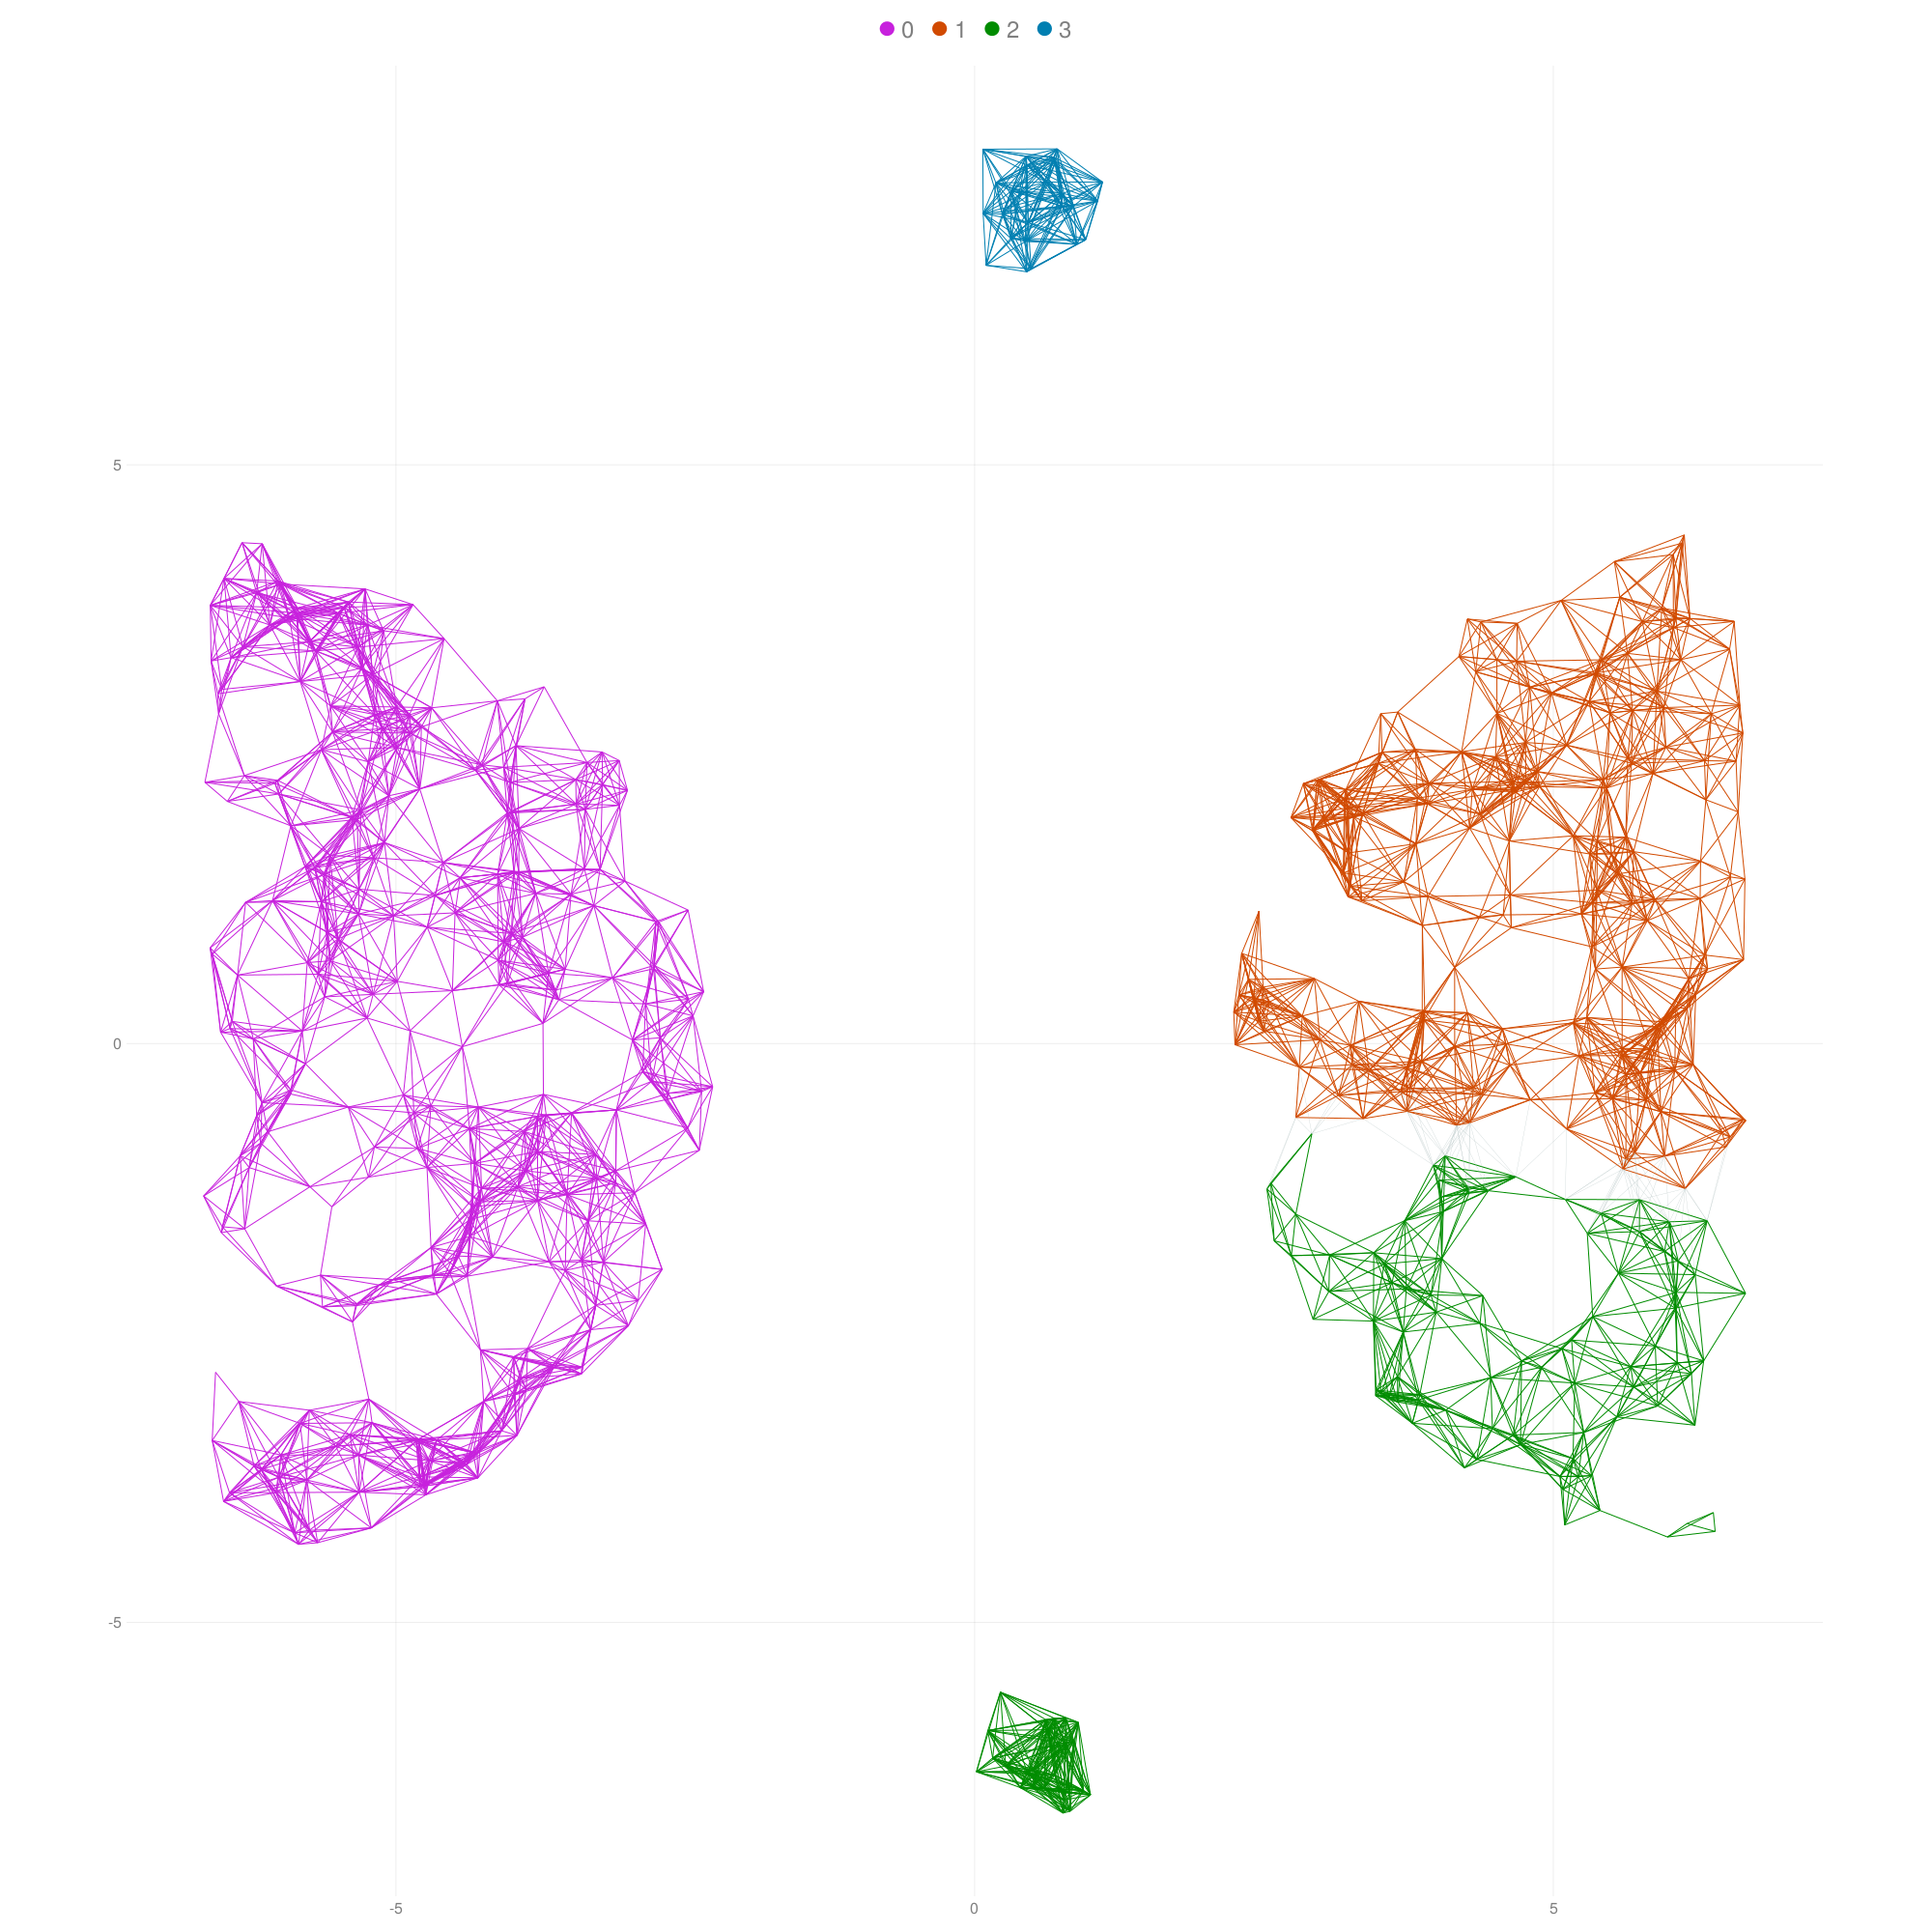
\includegraphics[height=0.4\linewidth]{fig/1/7.'pts_outlier'-K4-kmeans.png}
        \caption{$\texttt {pts\_outlier}$ $k$-means clustering.}
            \label{fig:pts_outlier-kmeans-k4}
    \end{minipage}
    \begin{minipage}{0.5\linewidth}
        \centering
        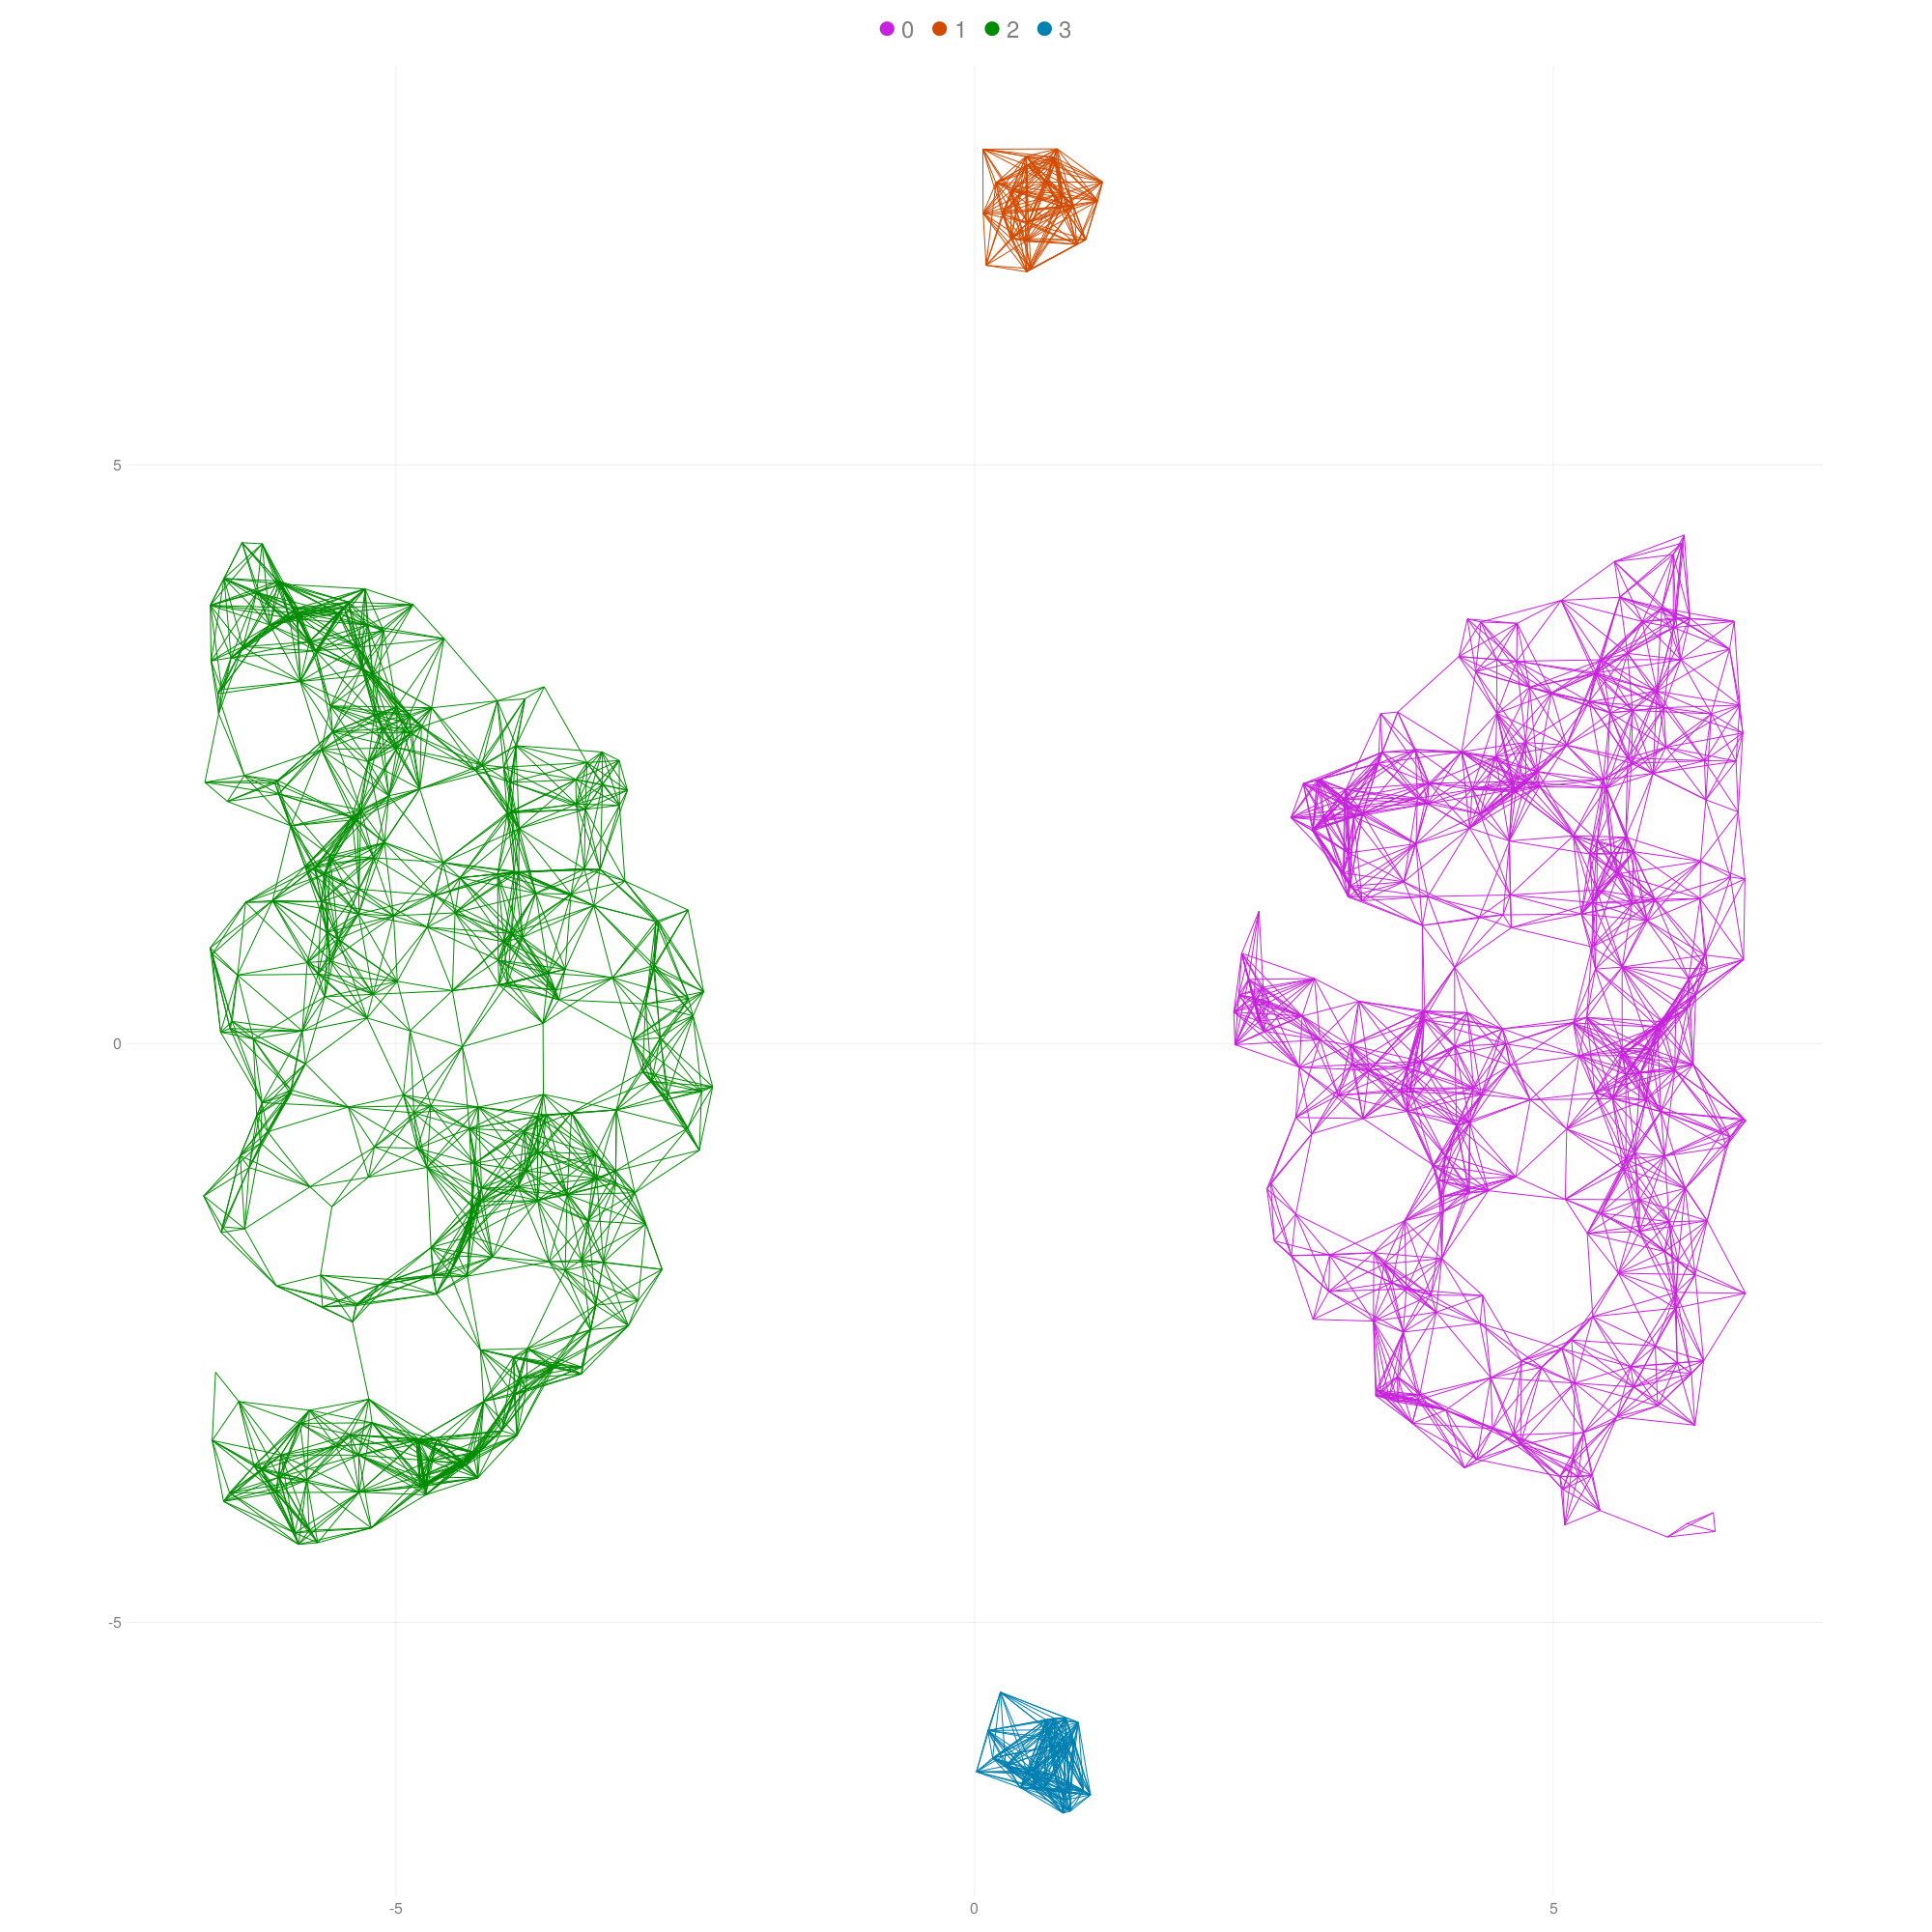
\includegraphics[height=0.4\linewidth]{fig/1/7.'pts_outlier'-K4-spectral.png}
        \caption{$\texttt {pts\_outlier}$ spectral clustering.}
    \end{minipage}
\end{minipage}
    \caption{Graph clustering for $K = 4$}
    \label{fig:clustering-k4}
\end{figure}\\

\section{Spectral clustering of real-world graphs [35 points]}
\subsection*{2.1. Computing the Laplacian Matrix and the eigenvector graph}
% TODO: Why do we necessarily grab the 2nd and 3rd eigen vectors ?
We compute the graph Laplacian matrix $L$ through the provided function and matrix $Y$ consisting of the eigenvectors associated with the $K$ smallest eigenvalues as usual.\\\\
We plot the graph with coordinates supplied by the $2$nd and $3$rd smallest eigenvalues, by definition:
$$ \centering
    (x_i,y_i) = (v_2(i), v_3(i))\quad \text{where $v_j$ is the eigenvector associated with the $j$th smallest eigenvalue }
$$
\begin{figure}[h!]
\begin{minted}[
frame=lines,
framesep=2mm,
]{julia}
    L, D = createlaplacian(W)

    lambda = eigvals(L);
    Y = eigvecs(L);
    ind = sortperm(lambda);
    Y = Y[:,ind[begin:K]]
    
    vertices = Y[:,2:3]
    draw_graph(W, vertices)
\end{minted}
\caption{Julia code for computing the Laplacian matrix and plotting the eigenvector graph}
\end{figure}\\
Below are some obtained plots:
\begin{figure}[h!]
    \begin{minipage}{0.5\linewidth}
        \centering
        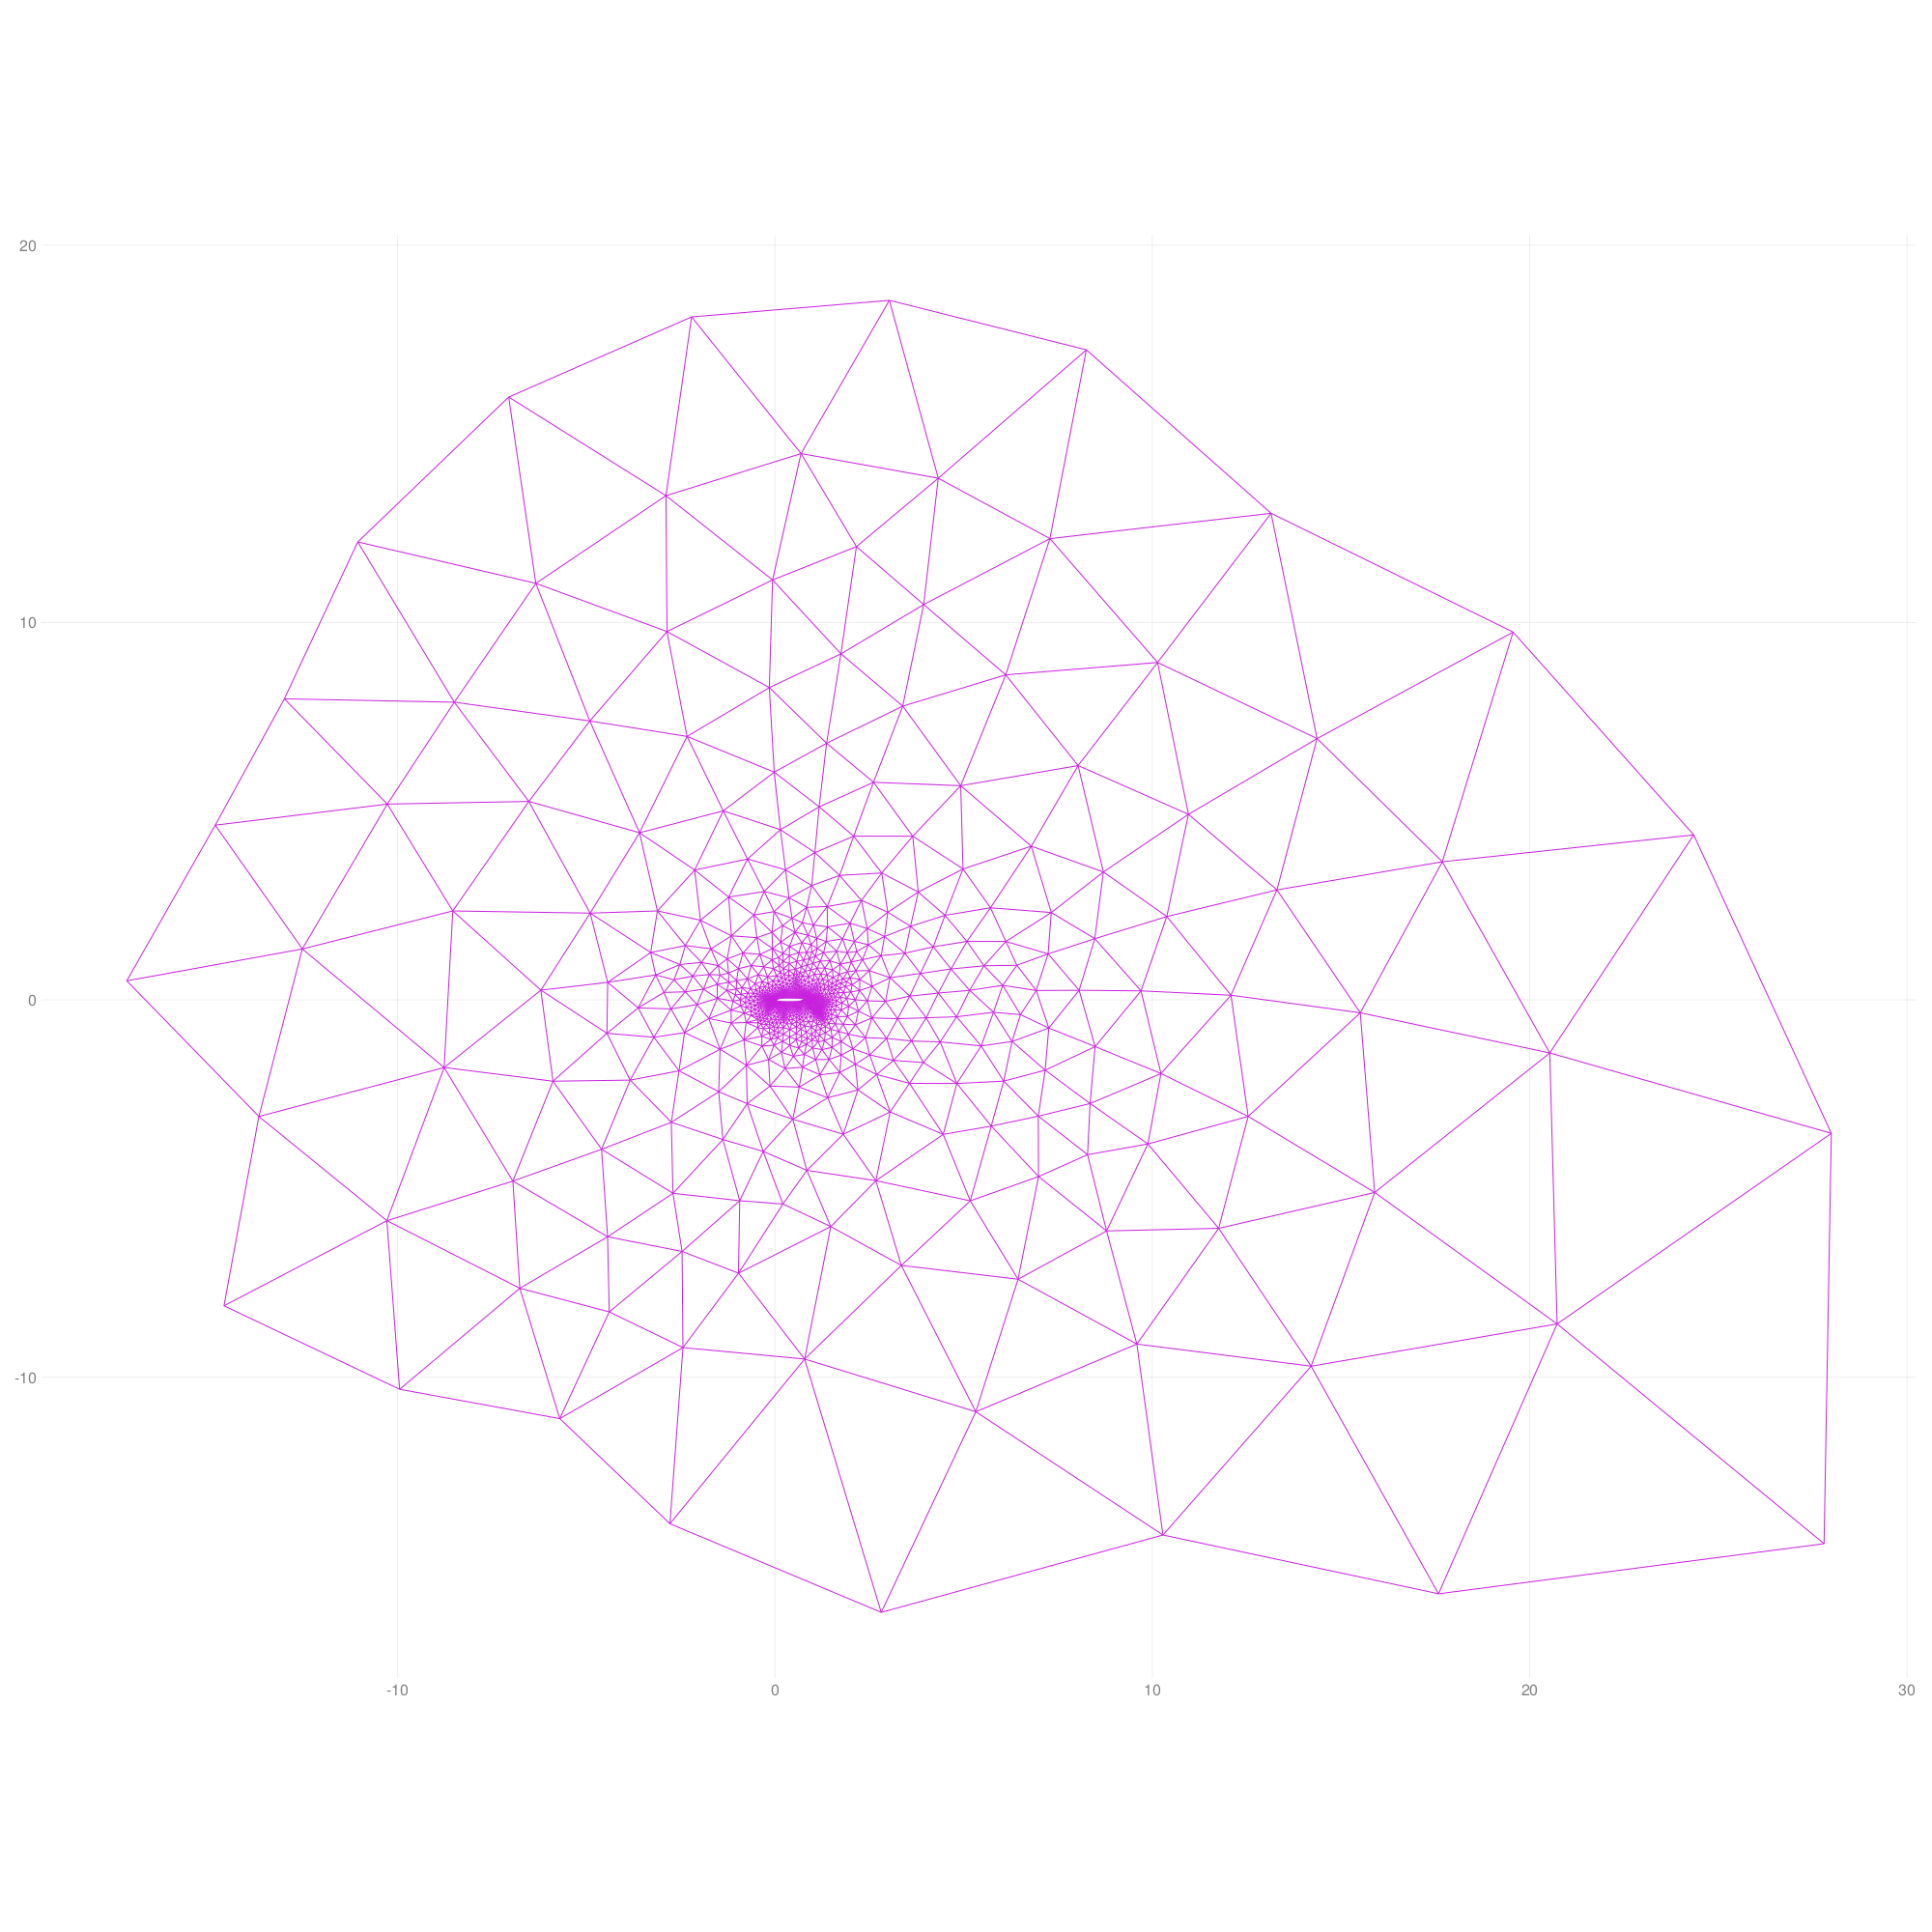
\includegraphics[height=0.7\linewidth]{fig/2/1.'barth4'-laplacian_plot.png}
    \end{minipage}
    \begin{minipage}{0.5\linewidth}
        \centering
        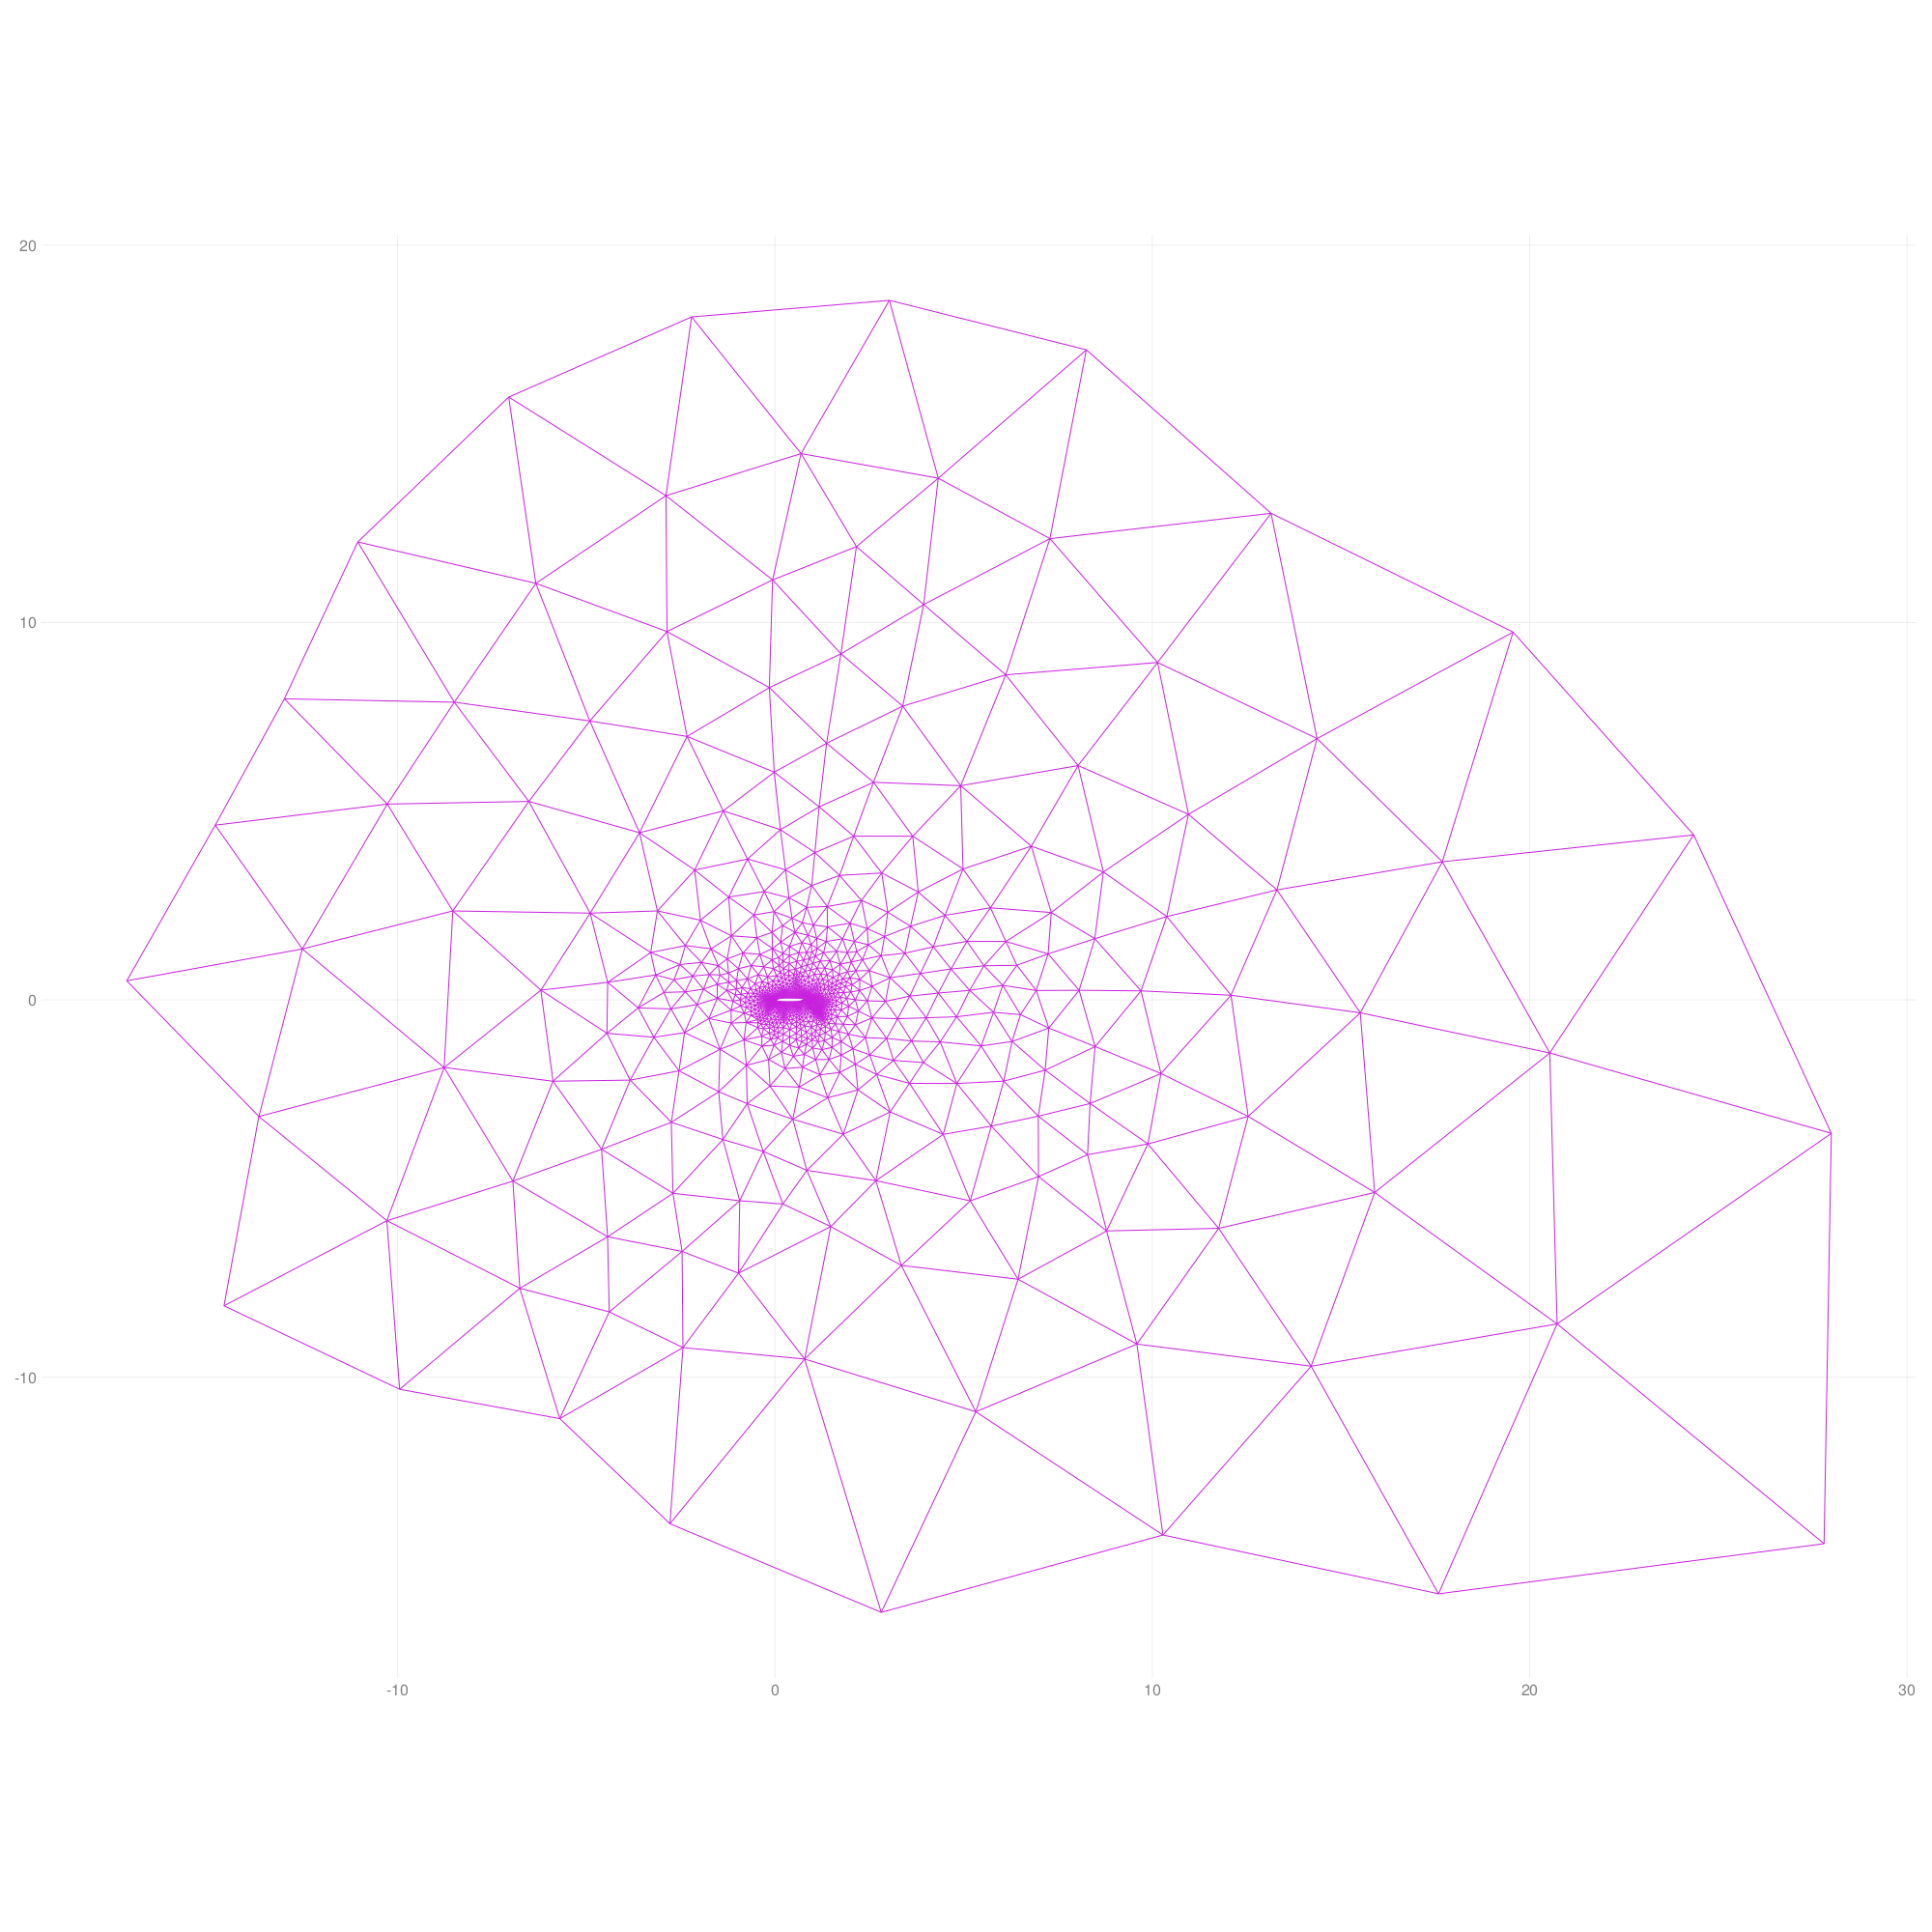
\includegraphics[height=0.7\linewidth]{fig/2/1.'barth4'-eigenvector_plot.png}
    \end{minipage}
        \caption{Visualization for $\texttt {barth4}$ graph, on the left the Laplacian matrix plot, on the right its eigenvector plot}
\end{figure}\\

\clearpage
\subsection*{2.2. Clustering each graph in $K=4$ clusters with the spectral and $k$-means method}
When plotting the provided graphs some clear differences between the two algorithms arise:\\
We know that basic $k$-means does not have the concept of a cluster density, and it really shows as the cartesian plane is divided into "areas" all of which have heterogeneous densities of points, leading to clusters that vary greatly in size.\\
For the \textit{Spectral method}, choosing a lower $K$ number of clusters may lead to clearly separate clusters to be clustered together and choosing a higher $K$ may lead to unnecessary fragmented clusters instead.
\begin{figure}[h!]
    \begin{minipage}{0.5\linewidth}
        \centering
        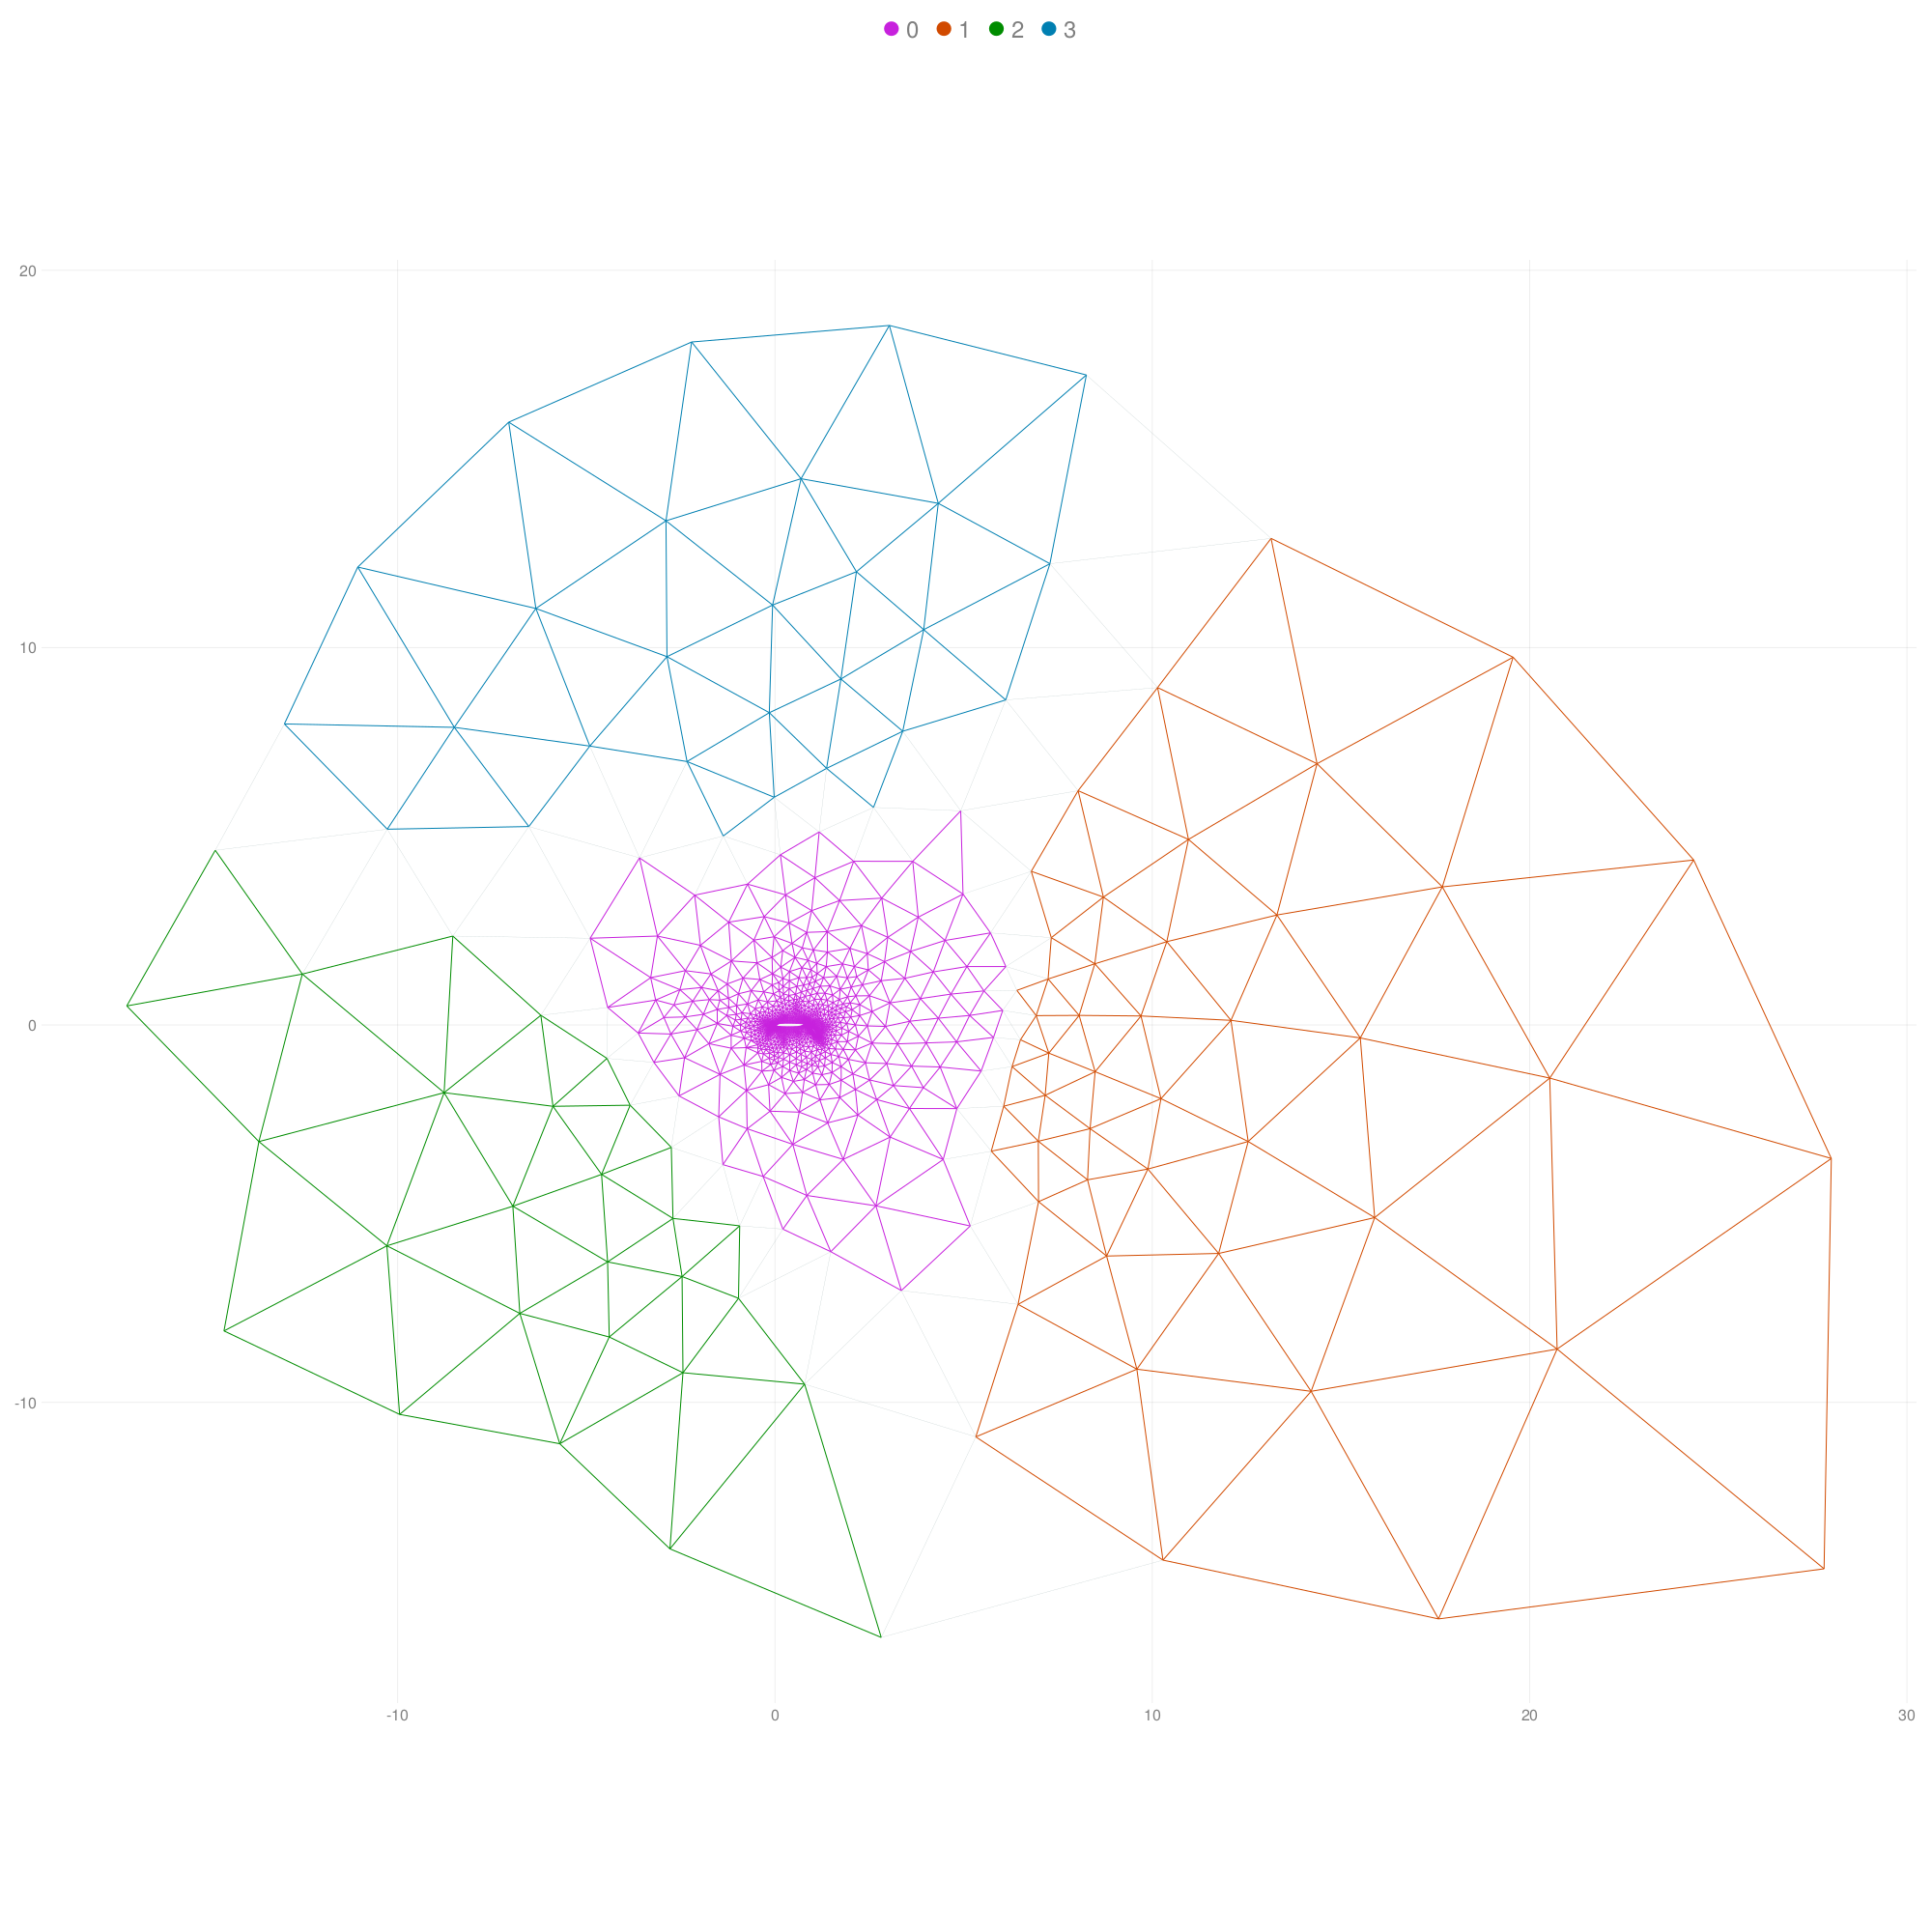
\includegraphics[height=0.5\linewidth]{fig/2/2.'barth4'-K4-kmeans.png}
    \end{minipage}
    \begin{minipage}{0.5\linewidth}
        \centering
        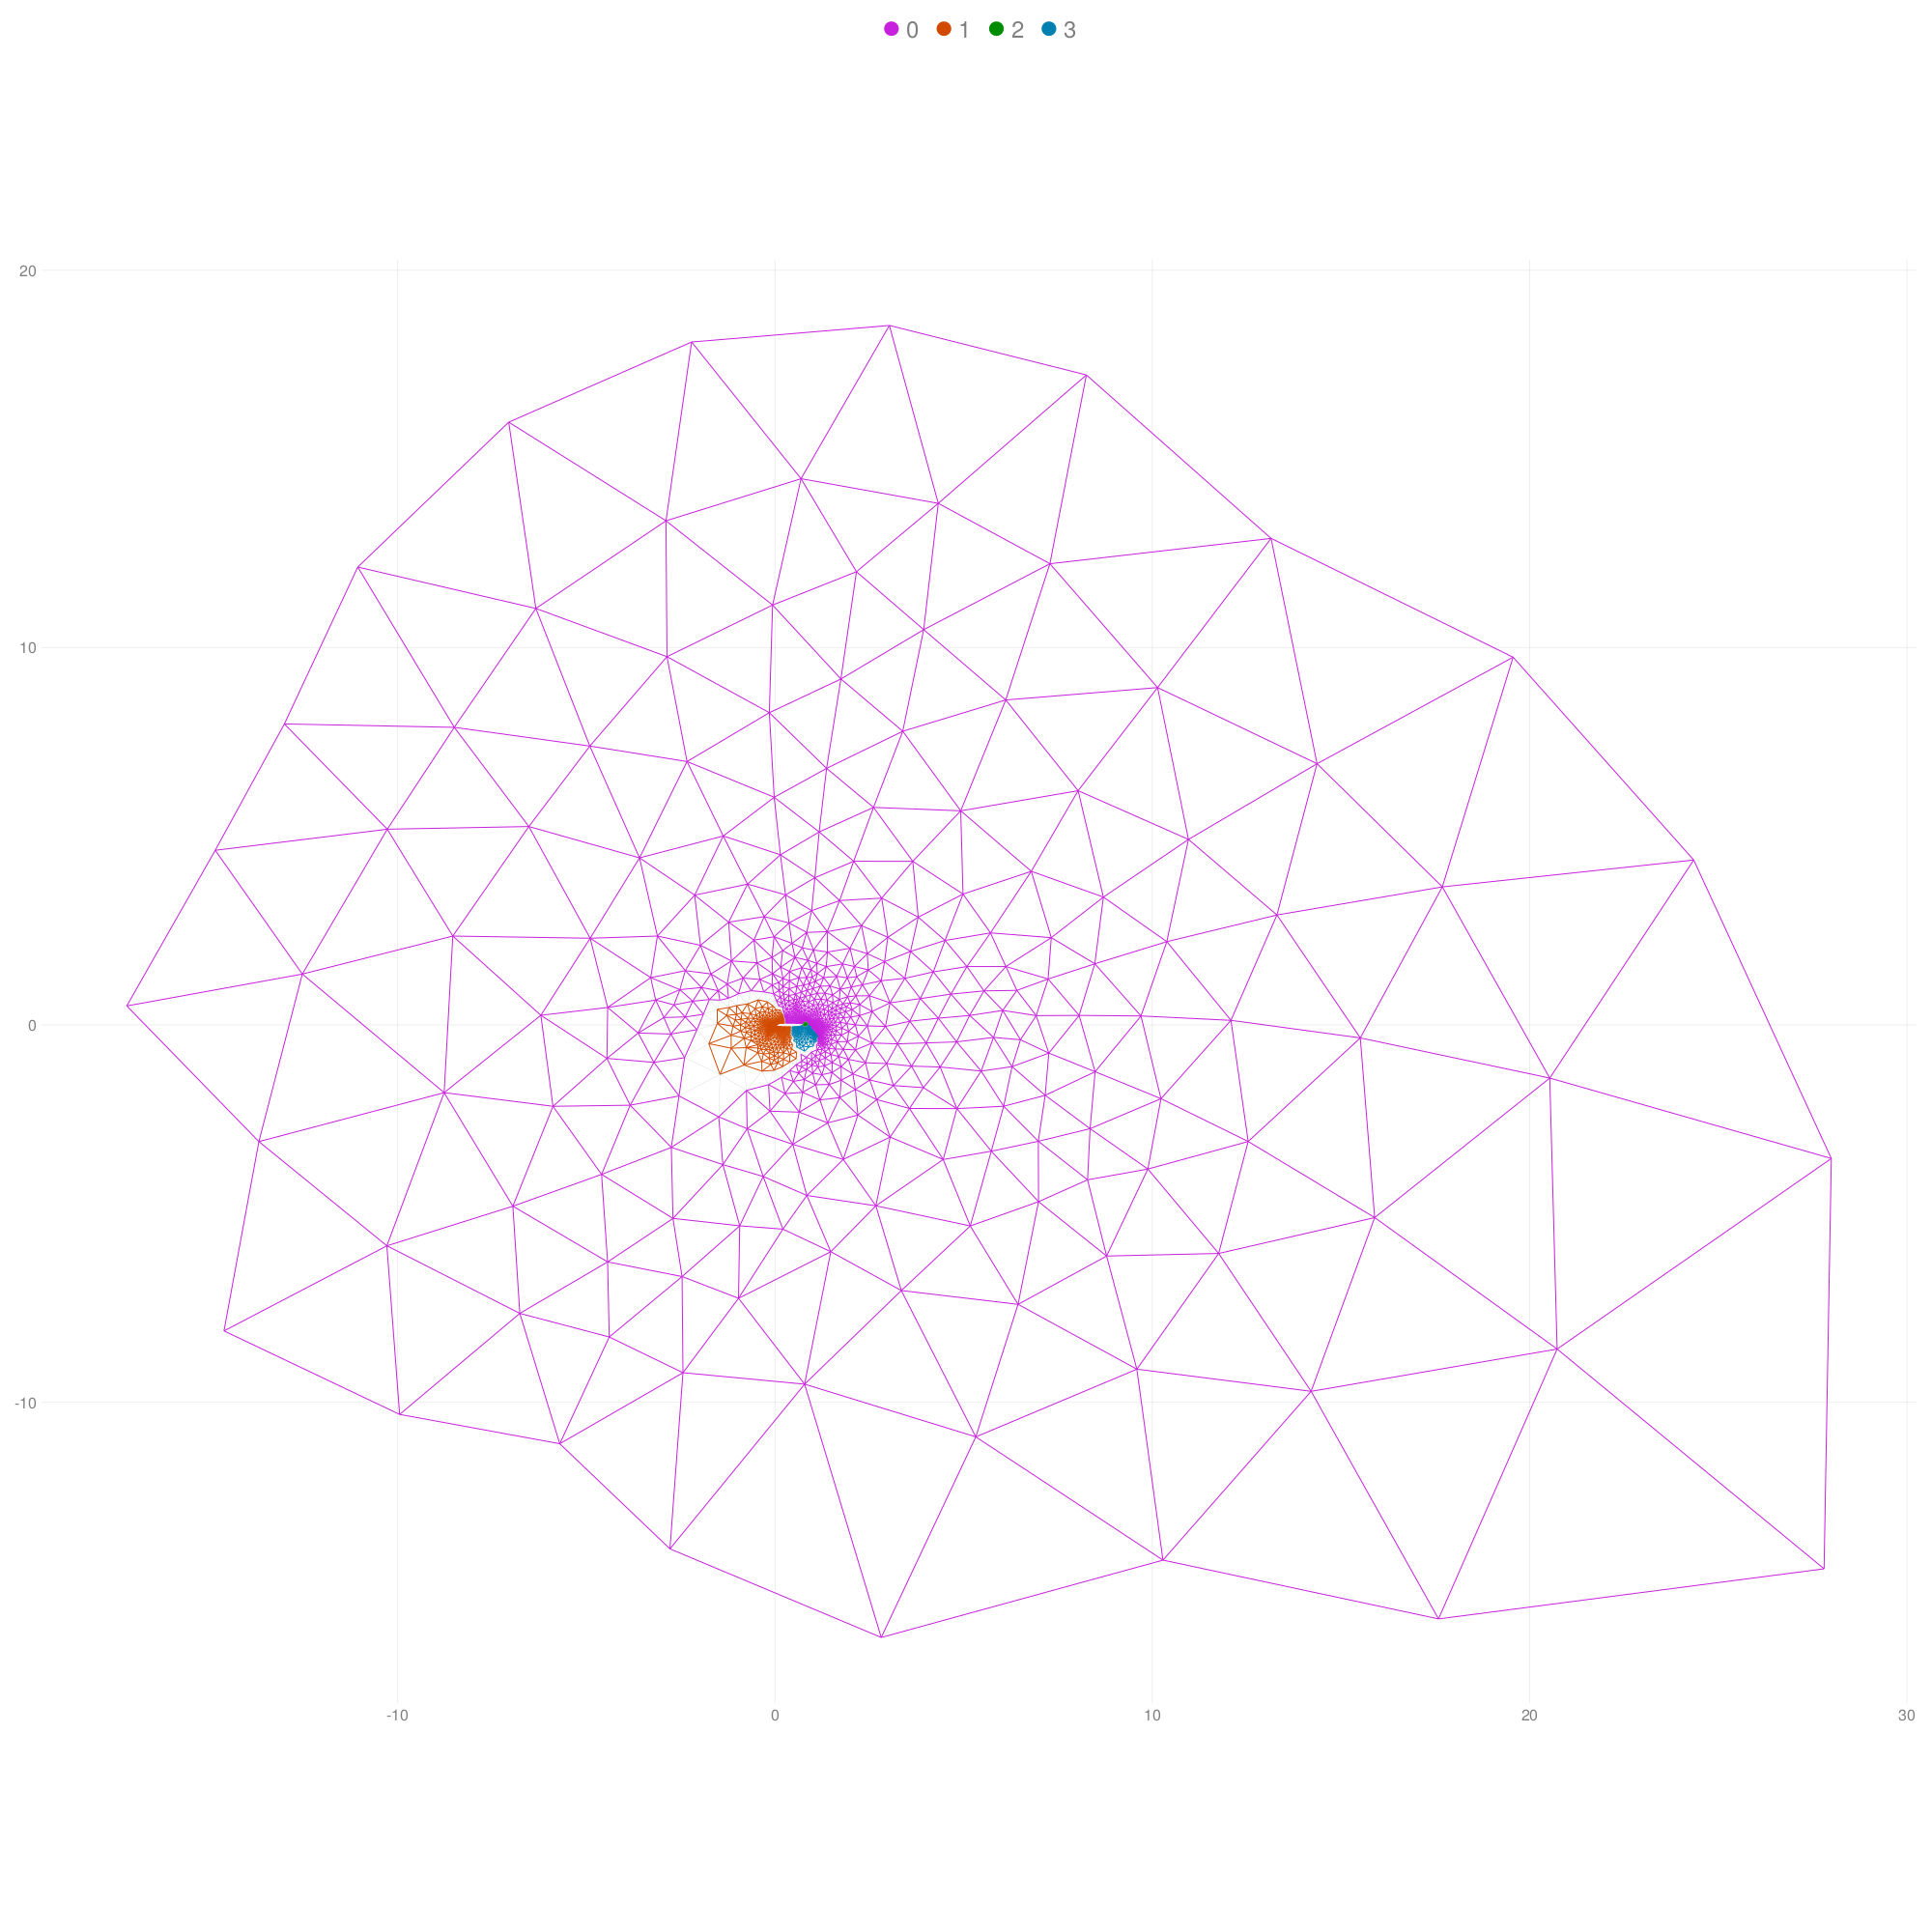
\includegraphics[height=0.5\linewidth]{fig/2/2.'barth4'-K4-spectral.png}
    \end{minipage}
    \caption{$\texttt {barth4}$ graph clustering. On the left with $k$-means clustering and on the right with spectral clustering, both for $K=4$.}
\end{figure}
\begin{figure}[h!]
    \begin{minipage}{0.5\linewidth}
        \centering
        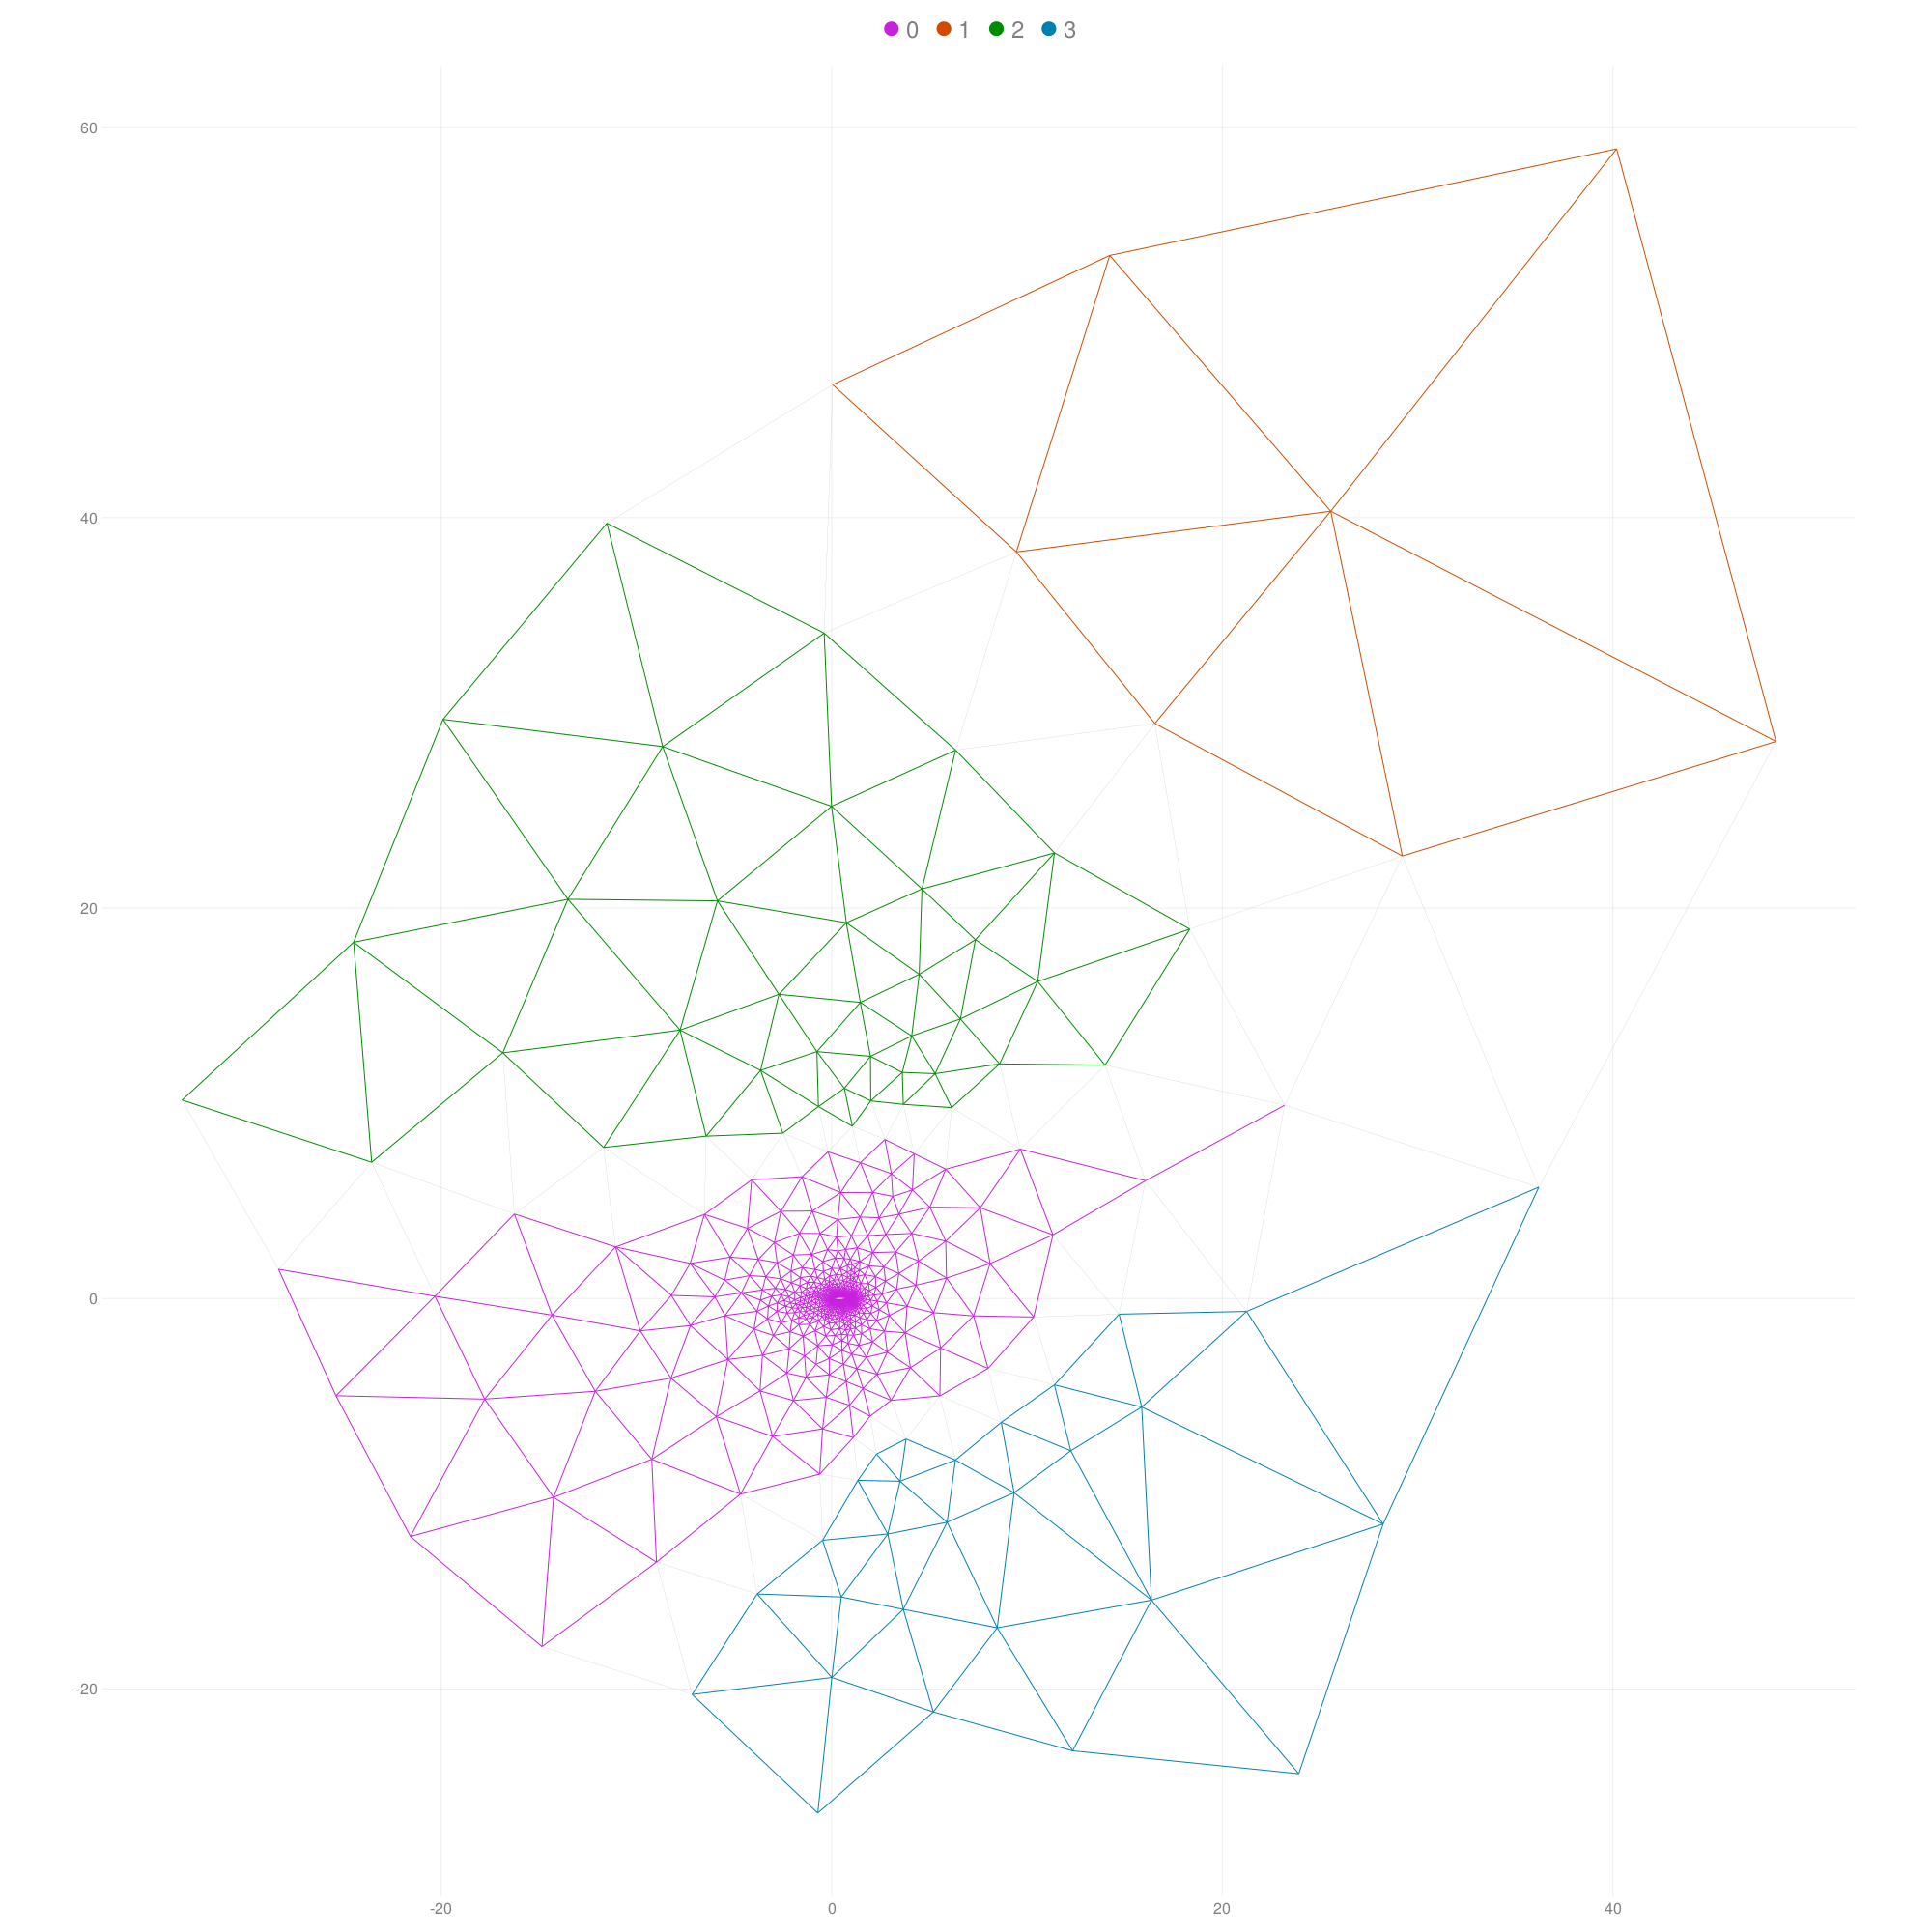
\includegraphics[height=0.5\linewidth]{fig/2/2.'3elt'-K4-kmeans.png}
    \end{minipage}
    \begin{minipage}{0.5\linewidth}
        \centering
        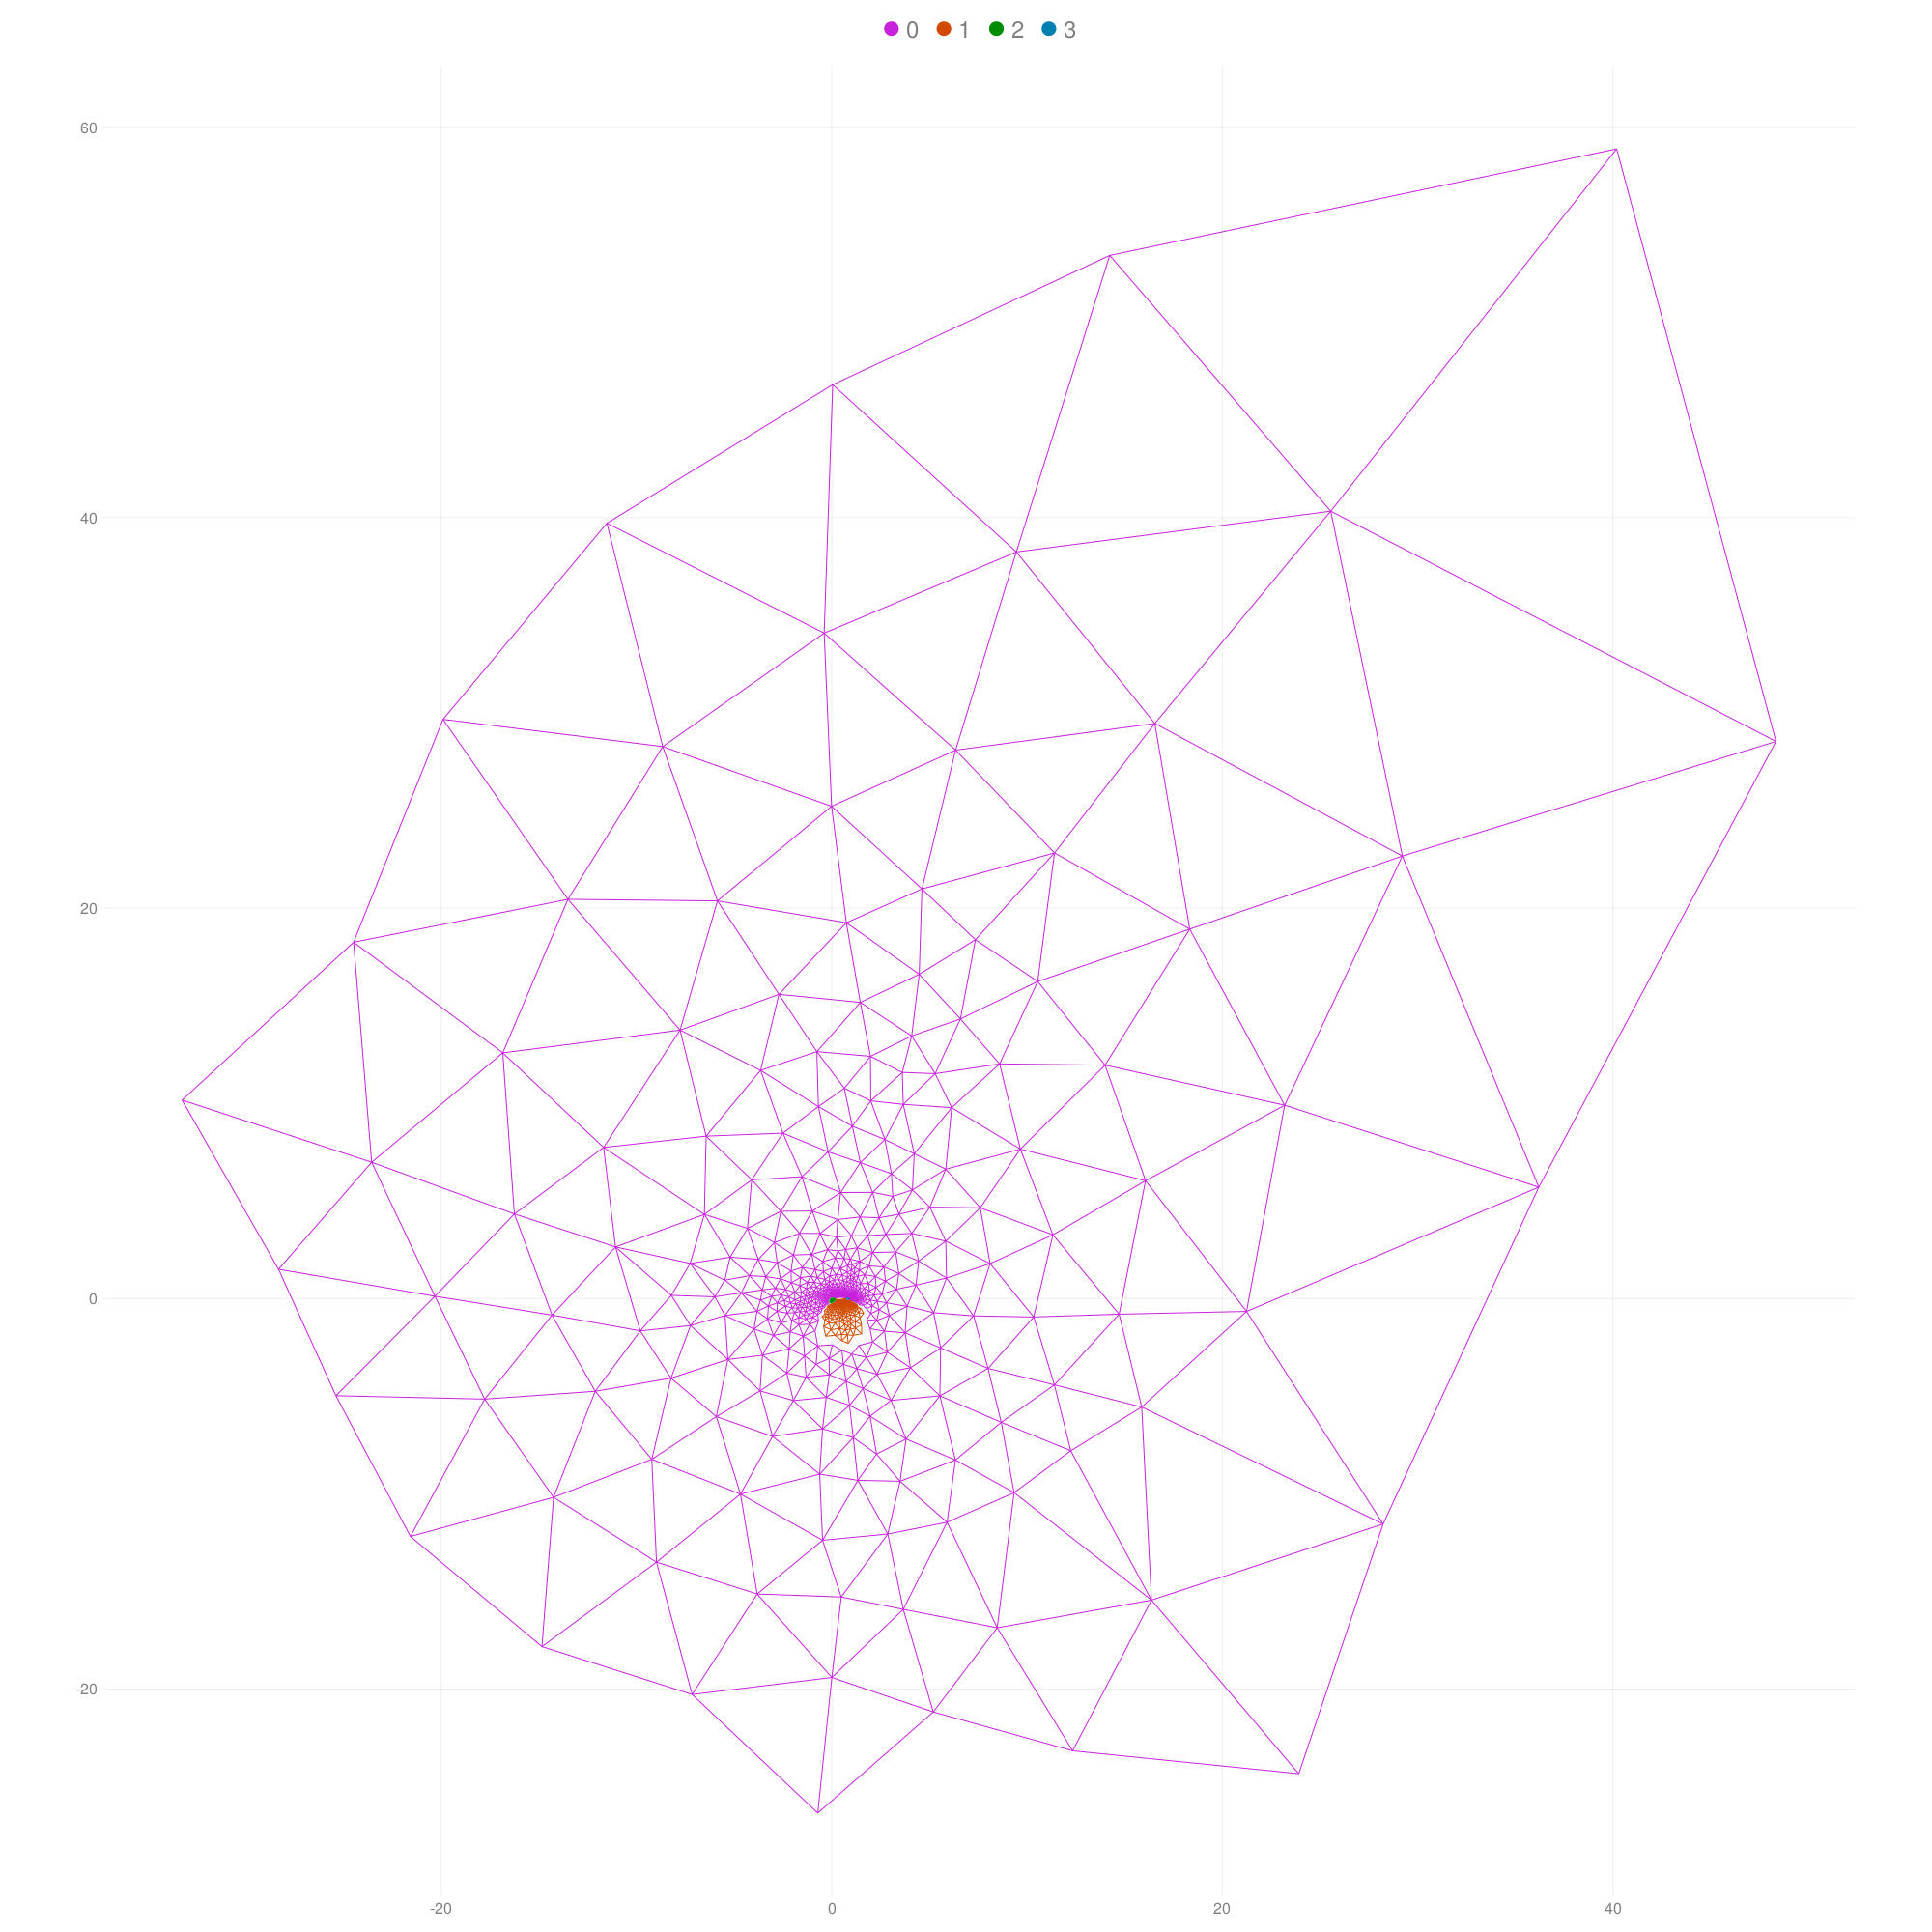
\includegraphics[height=0.5\linewidth]{fig/2/2.'3elt'-K4-spectral.png}
    \end{minipage}
    \caption{$\texttt {3elt}$ graph clustering. On the left with $k$-means clustering and on the right with spectral clustering, both for $K=4$.}
\end{figure}
\begin{figure}[h!]
    \begin{minipage}{0.5\linewidth}
        \centering
        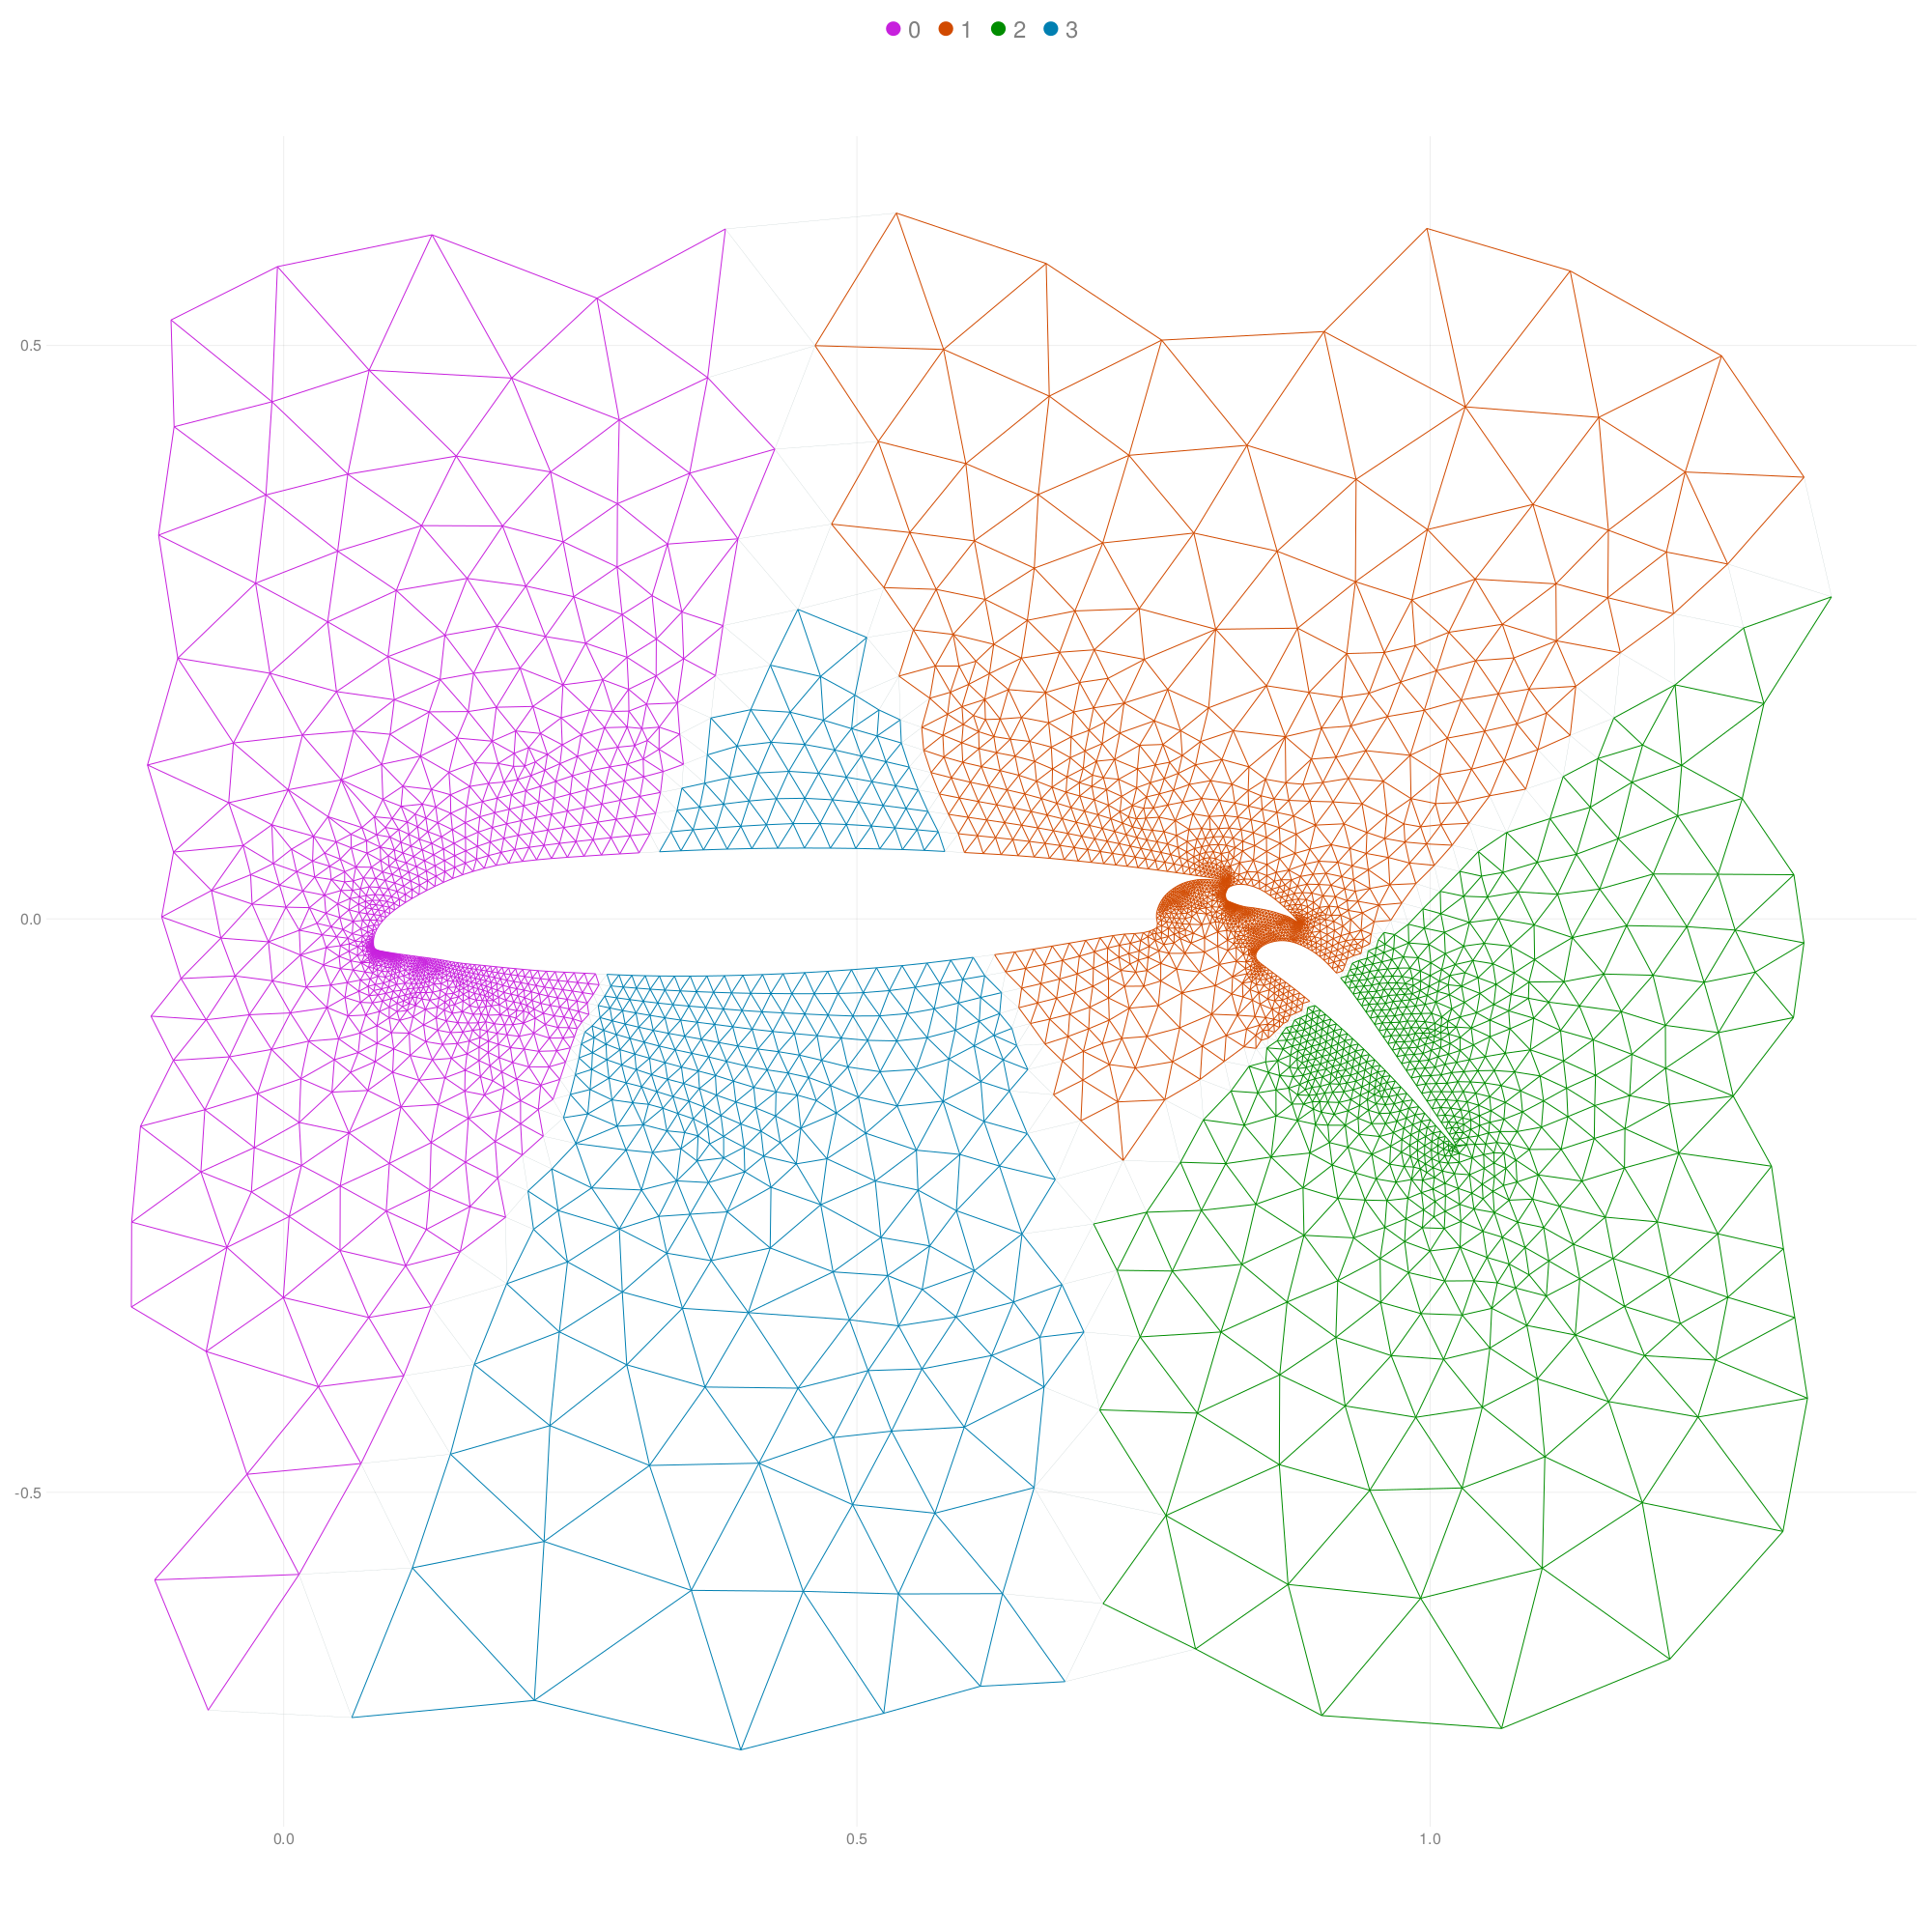
\includegraphics[height=0.5\linewidth]{fig/2/2.'airfoil1'-K4-kmeans.png}
    \end{minipage}
    \begin{minipage}{0.5\linewidth}
        \centering
        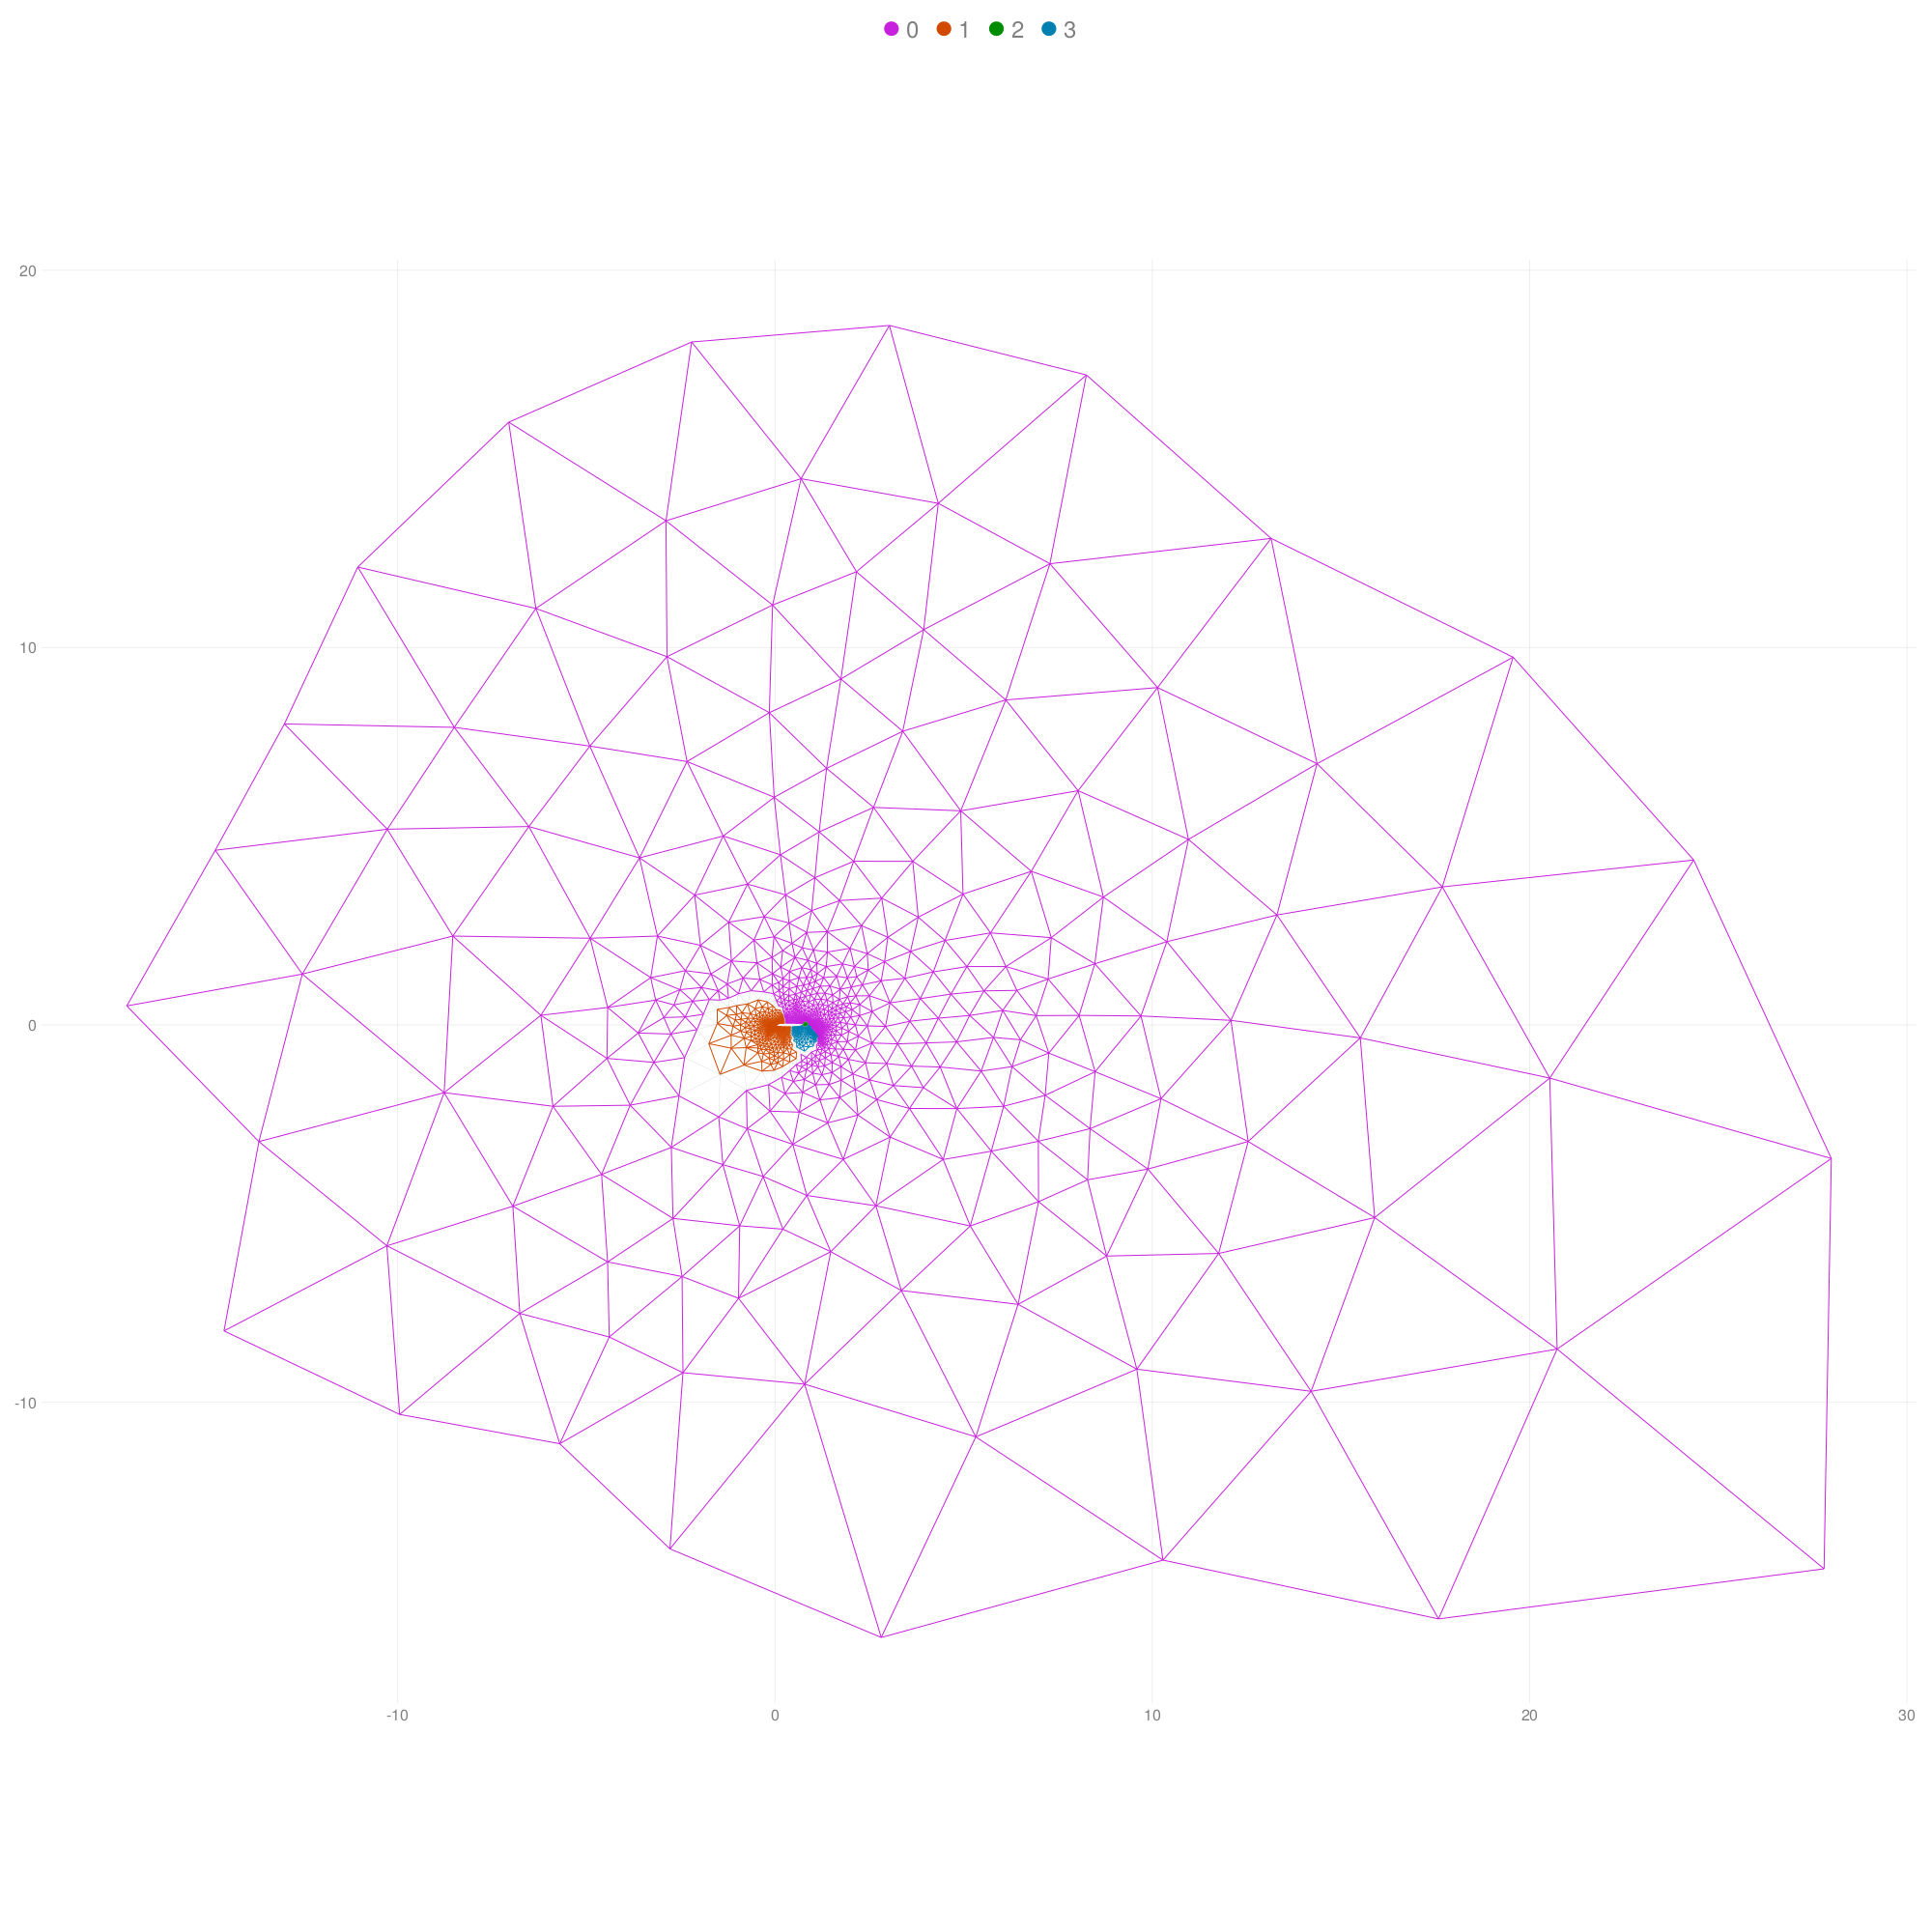
\includegraphics[height=0.5\linewidth]{fig/2/2.'barth4'-K4-spectral.png}
    \end{minipage}
    \caption{$\texttt {airfoil1}$ graph clustering. On the left with $k$-means clustering and on the right with spectral clustering, both for $K=4$.}
\end{figure}

\clearpage
\subsection*{2.3. Cluster size comparison}
As stated before, the obvious difference between the two algorithms is that the basic $k$-means algorithm lacks knowledge of cluster density, partitioning the points based solely on their spacial distance. This results in clusters that are extremely heterogeneous in size.
\begin{figure}[h!]

\begin{minipage}{\textwidth}
    \begin{minipage}{0.5\linewidth}
        \centering
        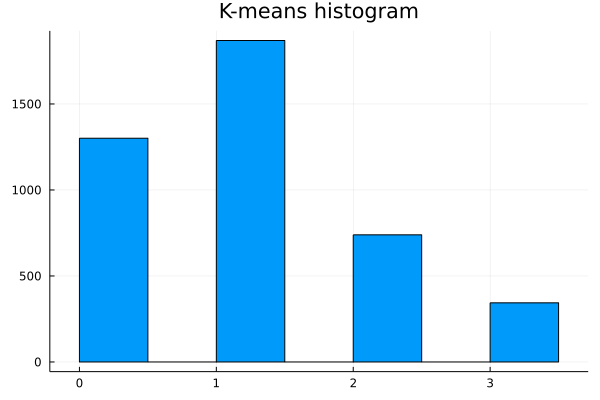
\includegraphics[height=0.6\linewidth]{fig/2/3.'airfoil1'-K4-kmeans_histogram.png}
        \caption{$\texttt {airfoil1}$ $k$-means clustering.}
    \end{minipage}
    \begin{minipage}{0.5\linewidth}
        \centering
        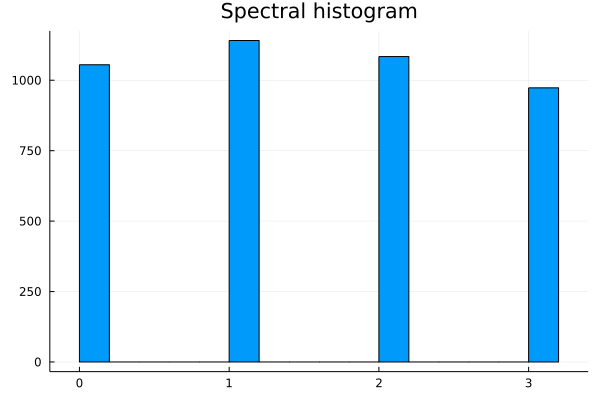
\includegraphics[height=0.6\linewidth]{fig/2/3.'airfoil1'-K4-spectral_histogram.png}
        \caption{$\texttt {airfoil1}$ spectral clustering .}
    \end{minipage}
    
    \begin{minipage}{0.5\linewidth}
        \centering
        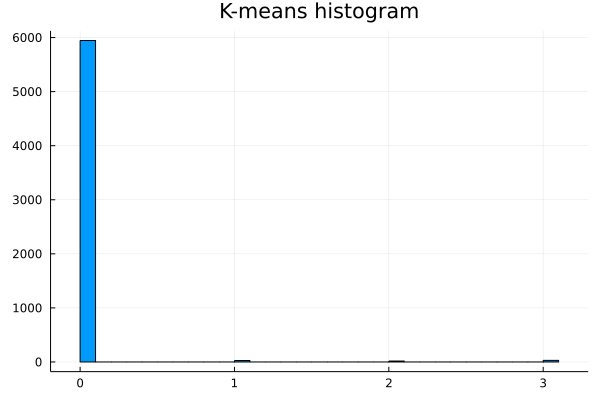
\includegraphics[height=0.6\linewidth]{fig/2/3.'barth4'-K4-kmeans_histogram.png}
        \caption{$\texttt {barth4}$ $k$-means clustering.}
    \end{minipage}
    \begin{minipage}{0.5\linewidth}
        \centering
        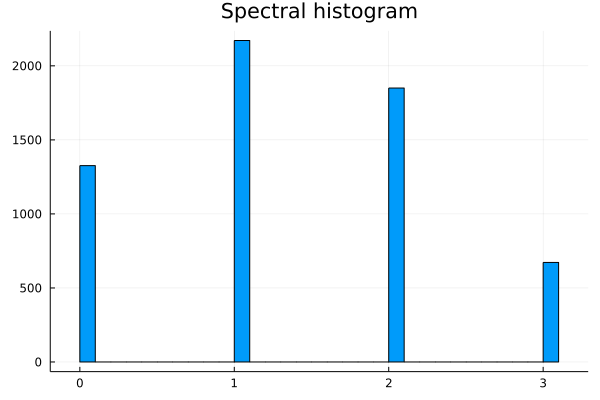
\includegraphics[height=0.6\linewidth]{fig/2/3.'barth4'-K4-spectral_histogram.png}
        \caption{$\texttt {barth4}$ spectral clustering.}
    \end{minipage}

    \begin{minipage}{0.5\linewidth}
        \centering
        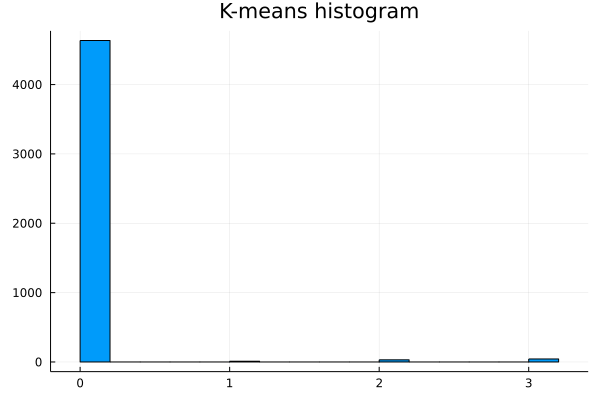
\includegraphics[height=0.6\linewidth]{fig/2/3.'3elt'-K4-kmeans_histogram.png}
        \caption{$\texttt {3elt}$ $k$-means clustering.}
    \end{minipage}
    \begin{minipage}{0.5\linewidth}
        \centering
        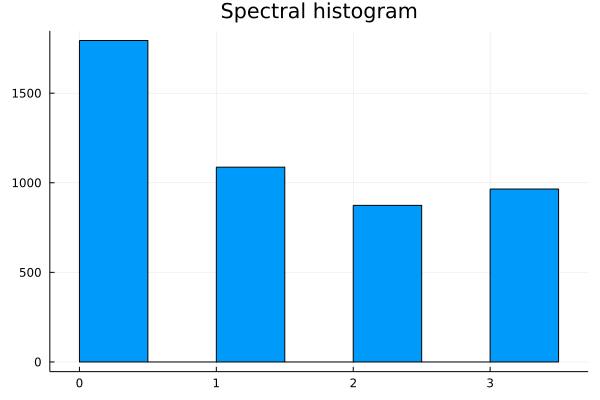
\includegraphics[height=0.6\linewidth]{fig/2/3.'3elt'-K4-spectral_histogram.png}
        \caption{$\texttt {3elt}$ spectral clustering.}
    \end{minipage}
\end{minipage}
\caption{Cluster size comparison with histograms}
\end{figure}
\begin{table}[h!]
    \centering
    \begin{tabular}{l|ll}
    Case &           Spectral &           K-Means \\ \hline
airfoil1 & 1055,1141,1084,973 & 2374,261,1293,325 \\
barth4 & 1326,2171,1850,672 &     5945,27,17,30 \\
3elt &  1794,1087,874,965 &      4644,8,40,28 \\
    \end{tabular}
    \caption{Cluster size comparison for $K=4$}
\end{table}

\clearpage
\section{Reproducing the obtained results}
In the \verb|src/| folder inside the submission archive you can find a \verb|Makefile|.\\\\
Run command \verb|make| while having the current working directory set as the \verb|src/| folder to plot and store all the results used for this report. All the plots and tables are saved inside the \verb|src/out| folder. Make sure to uncomment the \verb|GLMakie.save(...)| statements for the plots you want to generate.\\\\
A known bug on my \verb|arm64| machine is the Julia REPL crashing unexpectedly for a segmentation error. Copying the code and pasting it in the Julia REPL running inside a standalone terminal prevents it from crashing for me.

\end{document}